% ********************************** %
% UNIVERSITE PARIS 8
% INSTITUT D'ENSEIGNEMENT À DISTANCE
% L2 LICENCE INFORMATIQUE
% 2024 - 2025

% RESEAUX %

% NOM: PULUDISU Mpia Mimpiya
% Numéro étudiant: 18913467
% ********************************** %

% Initialisation du document de type "article"
% format A4 et des marges de 1.8 cm sur chaque côté.
\documentclass[a4paper,11pt]{article}
\usepackage[a4paper, margin=1.8cm]{geometry}
% Encodage de caractère
\usepackage[T1]{fontenc}
% Définit l'encodage UTF-8
\usepackage[utf8]{inputenc}
% Permet la gestion des particularités linguistiques
% propres à la langue française
\usepackage[french]{babel}
% Pour la gestion de couleurs
\usepackage{xcolor}
% Permet la personalisation de la table de matières
\usepackage{tocloft}
% sert à personnaliser les listes
\usepackage{enumitem}
% Pour gérer les liens hypertextes et urls
\usepackage{hyperref}
% Pour les fonctionnalités mathématiques
\usepackage{amsmath}
% Ajoute les polices mathématiques
\usepackage{amsfonts}
% Gère les images
\usepackage{graphicx}
 % Pour gérer les citations et les guillemets
\usepackage[style=english]{csquotes}
% Permet la gestion de tableaux extensibles
\usepackage{tabularx}
% Pour fusionner les cellules sur plusieurs lignes dans un tableau
\usepackage{multirow}

\usepackage{listings}

\usepackage{upquote}

\usepackage{tcolorbox}

\usepackage{verbatim}

\usepackage{caption}


% Indique l'auteur du document
\author{Mpia Mimpiya PULUDISU\\Noméro étudiant: 18913467\\L2 Informatique}

% Indique le titre du document
\title{\LARGE{Réalisation du programme \\ \vspace{2.8cm} \textcolor{blue}{EcoTrace}\\ Calculateur d'Empreinte Carbone Personnelle\vspace{2.5cm}}}

% Je défini la date au 15 décembre 2020 comme demandé dans le devoir
% On peut également mettre la date de la dernière compilation : \date{\today}
\date{\today}

% Personalisation de la table de matières
% change la couleur de texte de sections et sous-sections en bleu et
% met les sections en gras
\renewcommand{\cftsecfont}{\color{blue}\normalfont}
\renewcommand{\cftsubsecfont}{\color{blue}\normalfont}
\renewcommand{\cftsecfont}{\bfseries}

% définit la couleur urls et liens hypertextes en bleu
\hypersetup{colorlinks=true,linkcolor=blue,urlcolor=blue}

% Définition de la configuration de base pour le langage Python
\lstset{
    language=Python,
    basicstyle=\ttfamily\small,
    keywordstyle=\color{blue}\bfseries,
    commentstyle=\color{gray},
    stringstyle=\color{red},
    numbers=none,
    numberstyle=\tiny\color{gray},
    stepnumber=1,
    numbersep=10pt,
    backgroundcolor=\color{gray!2},
    tabsize=4,
    captionpos=b,
    breaklines=true,
    breakatwhitespace=false,
    showspaces=false,
    showstringspaces=false,
    showtabs=false,
    frame=single,
    framesep=10pt,
    framerule=0.1pt,
    aboveskip=10pt,
    belowskip=10pt,
    inputencoding=utf8,
    extendedchars=true,
    literate=%
        {é}{{\'e}}1
        {è}{{\`e}}1
        {à}{{\`a}}1
        {ç}{{\c{c}}}1
        {ê}{{\^e}}1
        {ë}{{\"e}}1
        {â}{{\^a}}1
        {î}{{\^i}}1
        {ï}{{\"i}}1
}

% Ajout de la prise en charge de CSS
\lstdefinelanguage{CSS}{
    keywords={color, background, background-color, border, margin, padding, font-size, font-family},
    sensitive=true,
    morecomment=[l]{//},
    morecomment=[s]{/*}{*/},
    morestring=[b]",
}

% Ajout de la prise en charge de HTML
\lstdefinelanguage{HTML}{
    language=html,
    sensitive=true,
    alsoletter={<>=-},
    morecomment=[s]{<!--}{-->},
    morestring=[b]",
    morekeywords={
      >, <, </, !, DOCTYPE, html, head, meta, link, script, body, div,
      h1, p, table, thead, tbody, tr, th, td, button, span, h1, h2, h3, h4,
      h5, h6, ul, ol, li, a, img, form, input, label, select, option, textarea,
      option, select
    }
}

% Ajout de la prise en charge de JavaScript
\lstdefinelanguage{JavaScript}{
    keywords={function, var, let, const, if, else, for, while, do, return, break, continue, switch, case, default, throw, try, catch, finally, new, this, typeof, instanceof, in, with, void, delete},
    sensitive=true,
    morecomment=[l]{//},
    morecomment=[s]{/*}{*/},
    morestring=[b]",
}

% Configuration pour Python (peut être redéfinie individuellement pour chaque langage si besoin)
\lstset{
    basicstyle=\ttfamily\small,
    keywordstyle=\color{blue}\bfseries,
    commentstyle=\color{gray},
    stringstyle=\color{red},
    backgroundcolor=\color{gray!2},
    frame=single,
    framesep=10pt,
    framerule=0.1pt,
    aboveskip=10pt,
    belowskip=10pt,
    tabsize=4,
    breaklines=true,
    breakatwhitespace=false,
    showspaces=false,
    showstringspaces=false,
    showtabs=false,
}


\tcbuselibrary{listingsutf8}


\begin{document}
    % Affiche le titre, l'auteur et la date
    \maketitle

    \vfill  % Push everything down

    % Place image directly without figure environment
    \noindent\makebox[\textwidth]{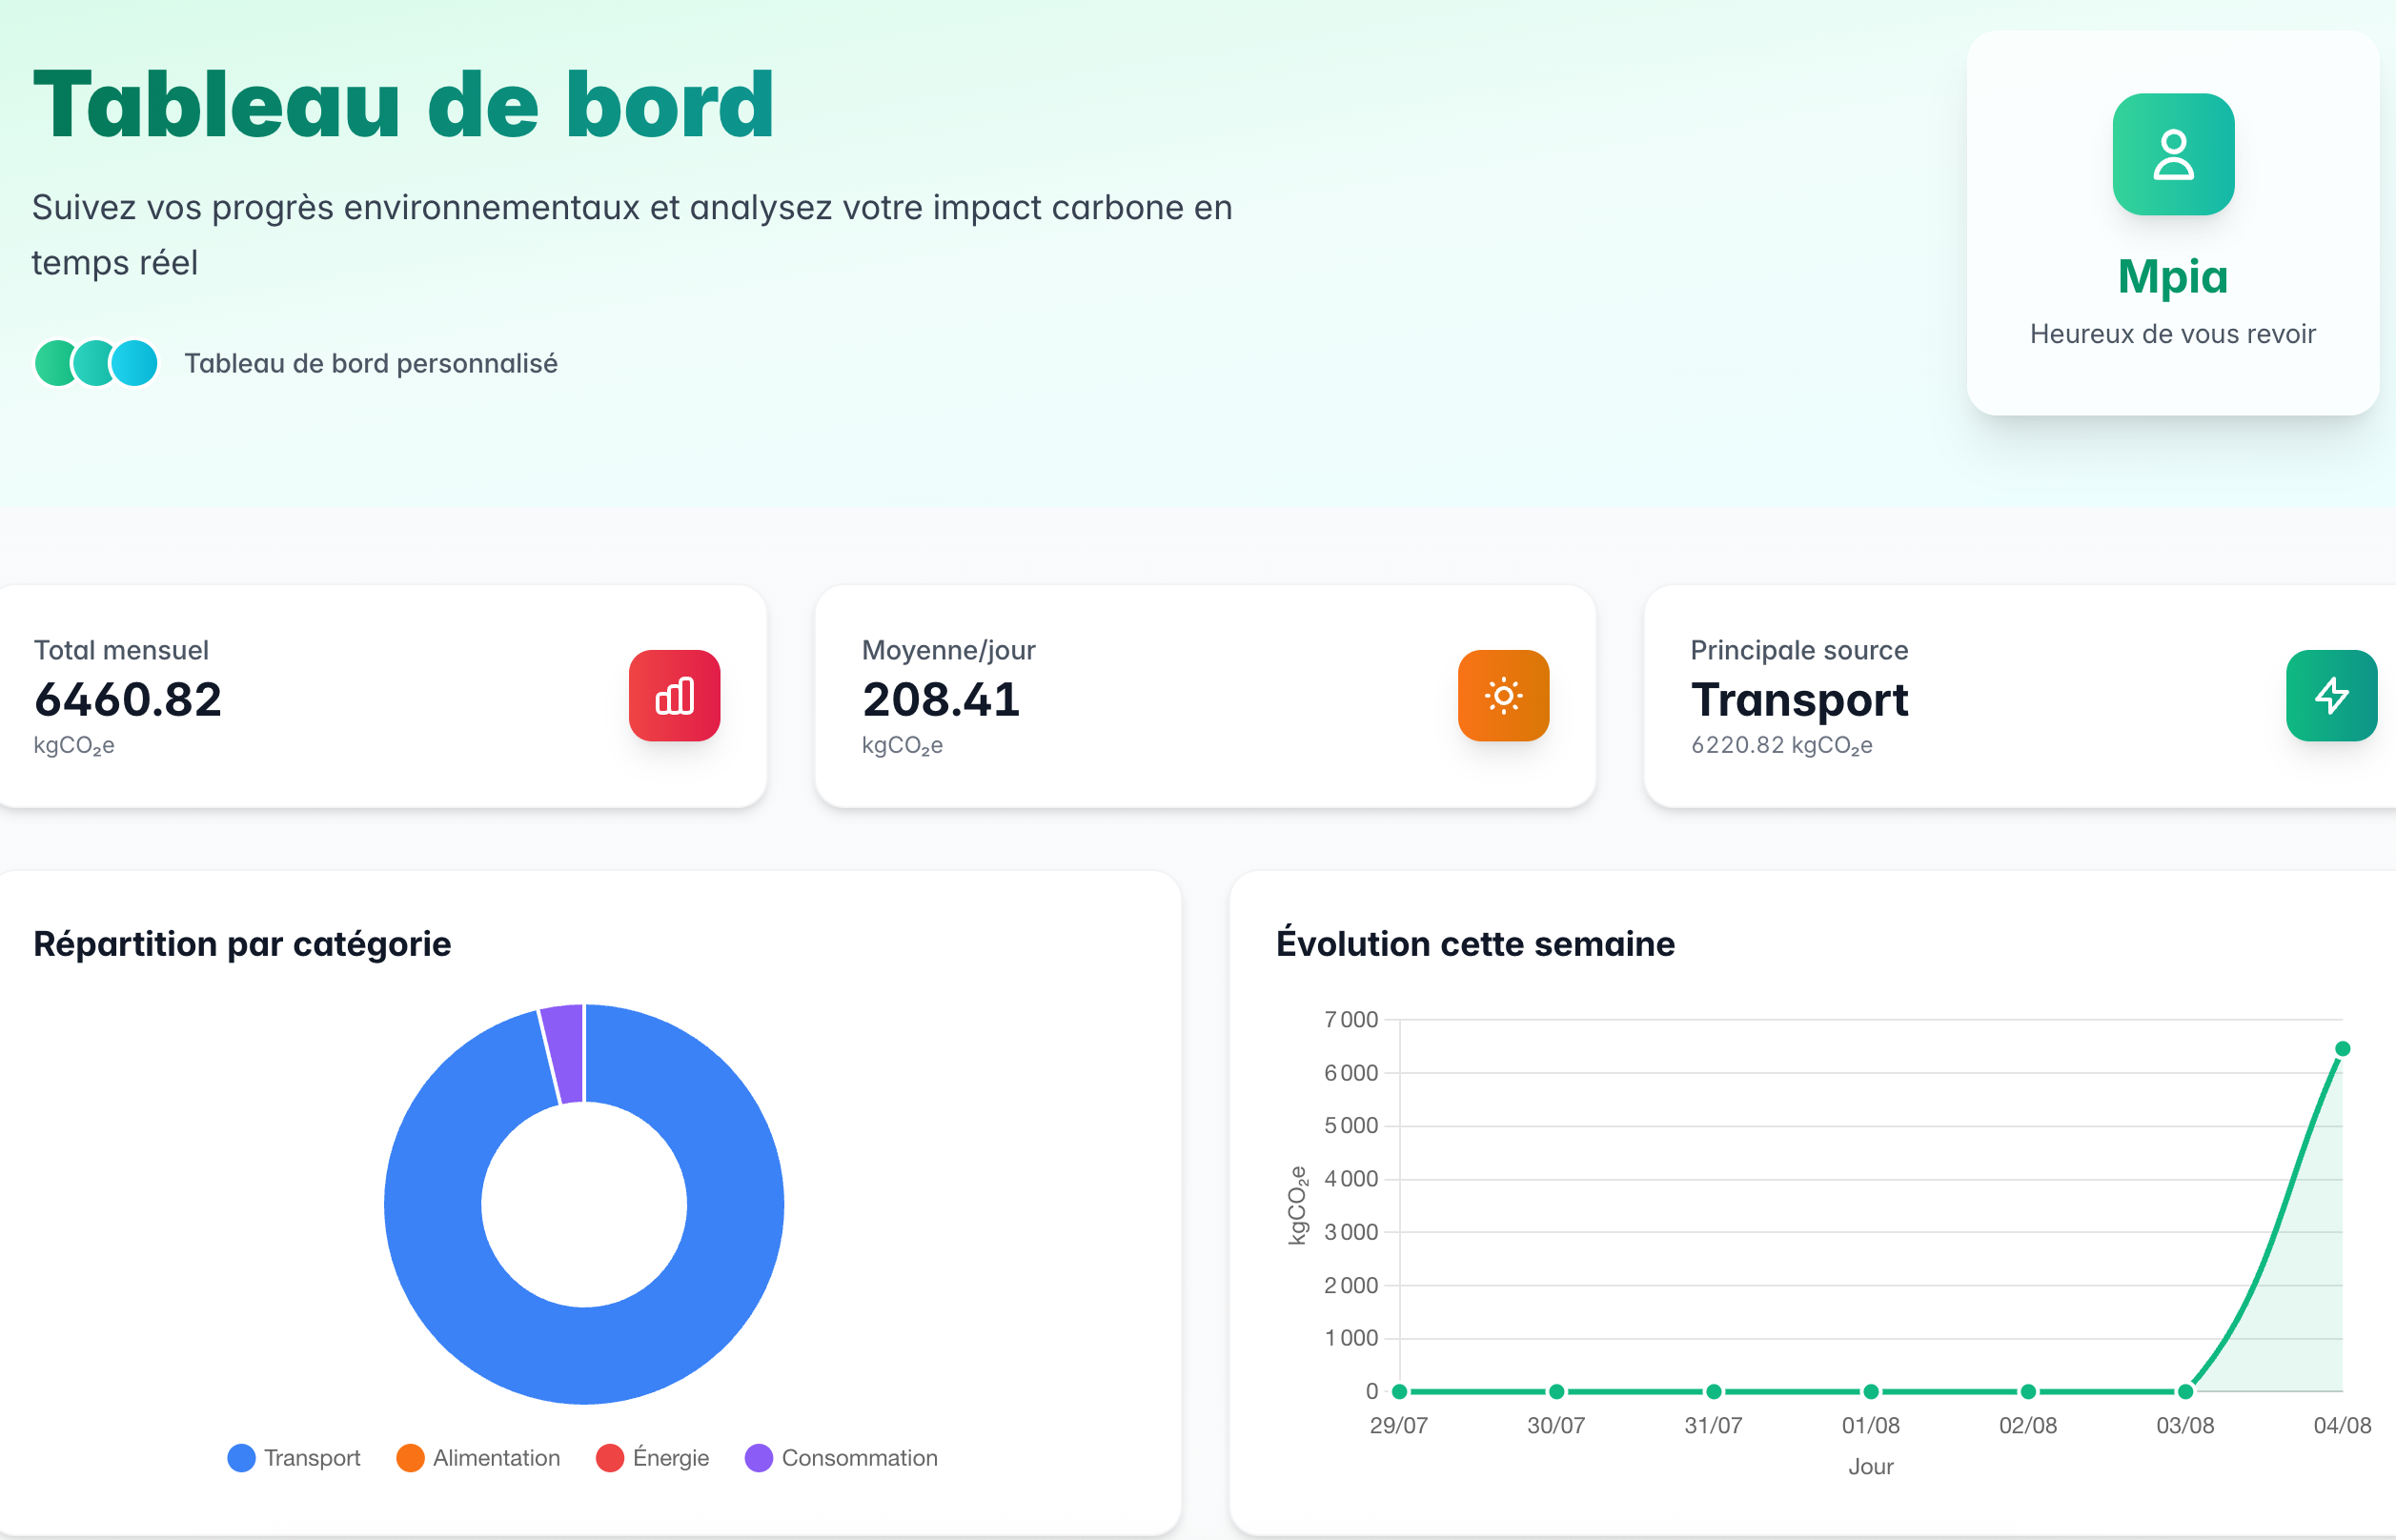
\includegraphics[width=\paperwidth]{screenshot.png}}

    % Table de matières
    \newpage
    \tableofcontents

    % Attendus du chapitre 10
    \newpage
    \section{Attendus du projet EcoTrace}

    \noindent EcoTrace est une application web permettant aux utilisateurs de calculer, suivre et réduire leur empreinte carbone personnelle à travers l'enregistrement d'activités quotidiennes (transport, alimentation, consommation d'énergie). Ce projet répond à une préoccupation environnementale actuelle tout en s'inscrivant dans un périmètre adapté à une réalisation individuelle.

    \subsection{Fonctionnalités principales}

    \begin{enumerate}
        \item \textbf{Calculateur d'empreinte carbone} :
            \begin{itemize}
                \item Interface pour saisir les activités quotidiennes et leurs quantités
                \item Base de données de facteurs d'émission pour différentes activités
                \item Algorithme de calcul additif ($émissions = quantité \times facteur\ d'émission$)
                \item Calcul automatique de l'impact carbone en temps réel
            \end{itemize}
            
        \item \textbf{Suivi des progrès} :
            \begin{itemize}
                \item Tableau de bord personnalisé avec statistiques en temps réel
                \item Visualisations par jour/semaine/mois avec Chart.js
                \item Répartition des émissions par catégorie (transport, alimentation, énergie, consommation)
                \item Historique complet des activités avec possibilité de tri et filtrage
            \end{itemize}
            
        \item \textbf{Recommandations personnalisées} :
            \begin{itemize}
                \item Moteur d'analyse automatique basé sur l'historique utilisateur
                \item Suggestions adaptées au profil d'émission de l'utilisateur
                \item Conseils pratiques pour réduire l'empreinte carbone
                \item Système de filtrage par impact et facilité de mise en œuvre
            \end{itemize}
    \end{enumerate}

    \subsection{Technologies et méthodologie}

    \begin{enumerate}
        \item \underline{Backend} : Python avec Flask, architecture MVC et programmation orientée objet
            \begin{itemize}
                \item Structure modulaire avec séparation des responsabilités
                \item Classes CarbonCalculator et RecommendationEngine pour la logique métier
                \item Gestion robuste des erreurs et validation des données
            \end{itemize}
            
        \item \underline{Frontend} : HTML/CSS avec TailwindCSS, JavaScript moderne, Chart.js pour visualisations
            \begin{itemize}
                \item Interface responsive et accessible
                \item Composants interactifs (calendrier personnalisé, dropdowns)
                \item Animations et micro-interactions pour l'engagement utilisateur
            \end{itemize}
            
        \item \underline{Base de données} : SQLite avec SQLAlchemy (ORM)
            \begin{itemize}
                \item Relations optimisées entre les tables
                \item Méthodes de classe pour les statistiques globales
                \item Initialisation automatique avec données ADEME
            \end{itemize}
            
        \item \underline{Source de données} : Utilisation des données de l'ADEME (\url{https://www.ademe.fr}) pour les facteurs d'émission CO2
            \begin{itemize}
                \item Facteurs d'émission officiels français
                \item Couverture complète des activités quotidiennes
                \item Données scientifiquement validées
            \end{itemize}
    \end{enumerate}

    \subsection{Structure de données simplifiée}

    \begin{table}[h!]
        \centering
        \caption{Structure simplifiée des tables de données principales}
        \begin{tabularx}{\textwidth}{|l|X|}
            \hline
            \textbf{Table} & \textbf{Champs} \\
            \hline
            Users & id, name, email, password, is\_admin, created\_at \\
            \hline
            Activities & id, user\_id, emission\_factor\_id, quantity, date, created\_at \\
            \hline
            EmissionFactors & id, category, subcategory, activity\_name, unit, co2\_factor, source \\
            \hline
        \end{tabularx}
    \end{table}

    \subsection{Réalisations techniques accomplies}

    \subsubsection{Architecture backend}
    \begin{itemize}
        \item \textbf{Module configs} : Configuration centralisée avec gestion d'erreurs et processeurs de contexte
        \item \textbf{Module controllers} : Classes CarbonCalculator et RecommendationEngine avec logique métier avancée
        \item \textbf{Module auth} : Système d'authentification complet avec Flask-Login et validation sécurisée
        \item \textbf{Module carbon} : Gestion des activités carbone avec validation multi-niveaux et cache LRU
    \end{itemize}

    \subsubsection{Interface utilisateur}
    \begin{itemize}
        \item \textbf{Templates responsive} : Design adaptatif avec TailwindCSS et composants réutilisables
        \item \textbf{JavaScript modulaire} : Scripts spécialisés pour chaque fonctionnalité avec optimisations
        \item \textbf{Visualisations} : Intégration Chart.js avec graphiques interactifs (doughnut, line, bar)
        \item \textbf{UX avancée} : Calendrier personnalisé, dropdowns stylisés, animations fluides
    \end{itemize}

    \subsubsection{Déploiement et production}
    \begin{itemize}
        \item \textbf{Déploiement réussi} : Application fonctionnelle sur PythonAnywhere
        \item \textbf{URL de production} : \url{https://ecotrace.pythonanywhere.com}
        \item \textbf{Code source} : \url{https://github.com/codewithmpia/ecotrace-l2}
        \item \textbf{Base de données initialisée} : Données \href{https://www.ademe.fr}{ADEME} intégrées et opérationnelles
        \item \textbf{Performance optimisée} : Minification automatique et lazy loading
    \end{itemize}

    \subsection{Conformité aux attendus}

    Le projet EcoTrace répond intégralement aux exigences initiales et les dépasse sur plusieurs aspects :

    \begin{itemize}
        \item \textbf{Fonctionnalités réalisées} : Les 3 fonctionnalités principales sont implémentées et fonctionnelles
        \item \textbf{Technologies respectées} : Stack technique conforme aux spécifications
        \item \textbf{Structure de données} : Modèle de données optimisé et extensible
        \item \textbf{Qualité du code} : Architecture professionnelle avec bonnes pratiques
        \item \textbf{Déploiement effectif} : Application accessible publiquement
    \end{itemize}


    % PARTIE I : LE MODULE CONFIGS
    \newpage
    \section{PARTIE I : Le module \texttt{configs}}
        \subsection{Structure générale du module}
            \noindent Le module \texttt{configs} constitue le coeur de la configuration de l'application EcoTrace. Il est organisé en quatre fichiers principaux :
            
            \begin{itemize}
                \item \texttt{\_\_init\_\_.py} : Fichier d'initialisation du module (vide mais indispensable)
                \item \texttt{settings.py} : Configuration principale de l'application
                \item \texttt{errors.py} : Gestion centralisée des erreurs
                \item \texttt{processors.py} : Processeurs de contexte pour les templates
            \end{itemize}

            \noindent Cette organisation respecte le principe de séparation des responsabilités, rendant la configuration modulaire et facile à maintenir.

            \begin{center}
                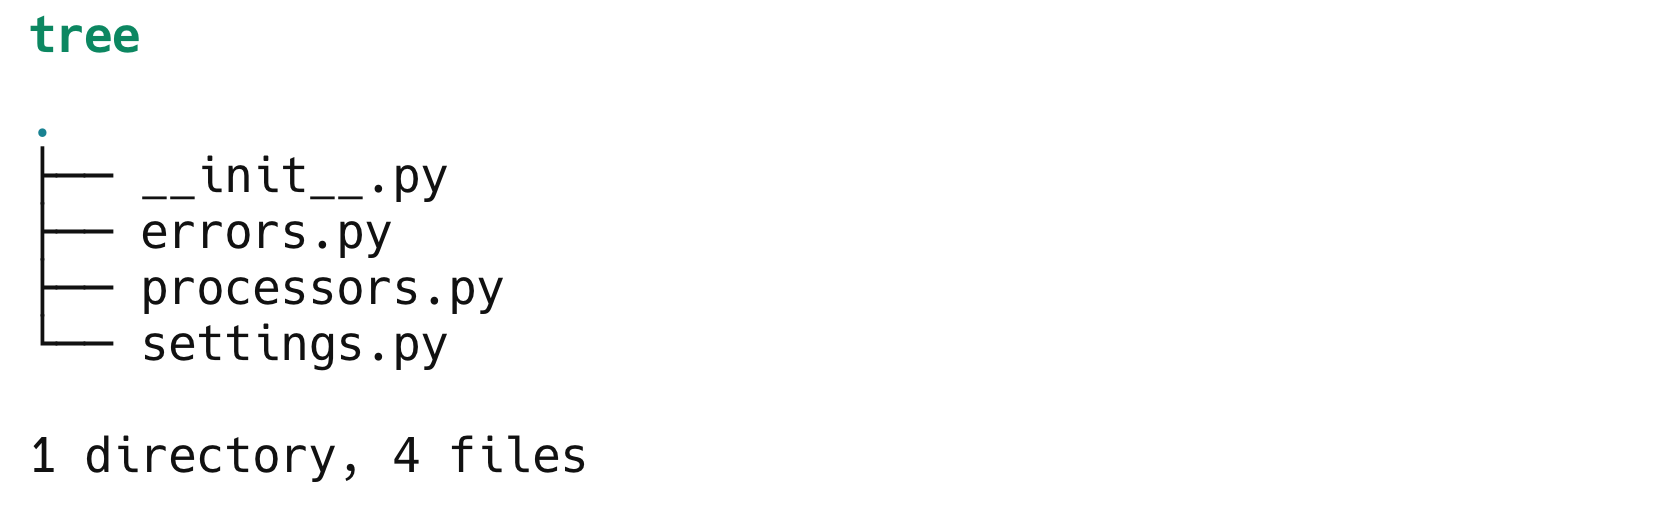
\includegraphics[width=0.7\textwidth]{captures/configs/img1.png}
            \end{center}

        \subsection{Configuration principale (\texttt{settings.py})}
            \noindent Le fichier \texttt{settings.py} contient la configuration centrale de l'application. Voici son contenu :

            \lstinputlisting[language=Python, caption={Code du module \texttt{settings.py} (configuration principale de l'application)}]{configs/settings.py}

            \noindent Les points clés de cette configuration sont :
            \begin{enumerate}
                \item \textbf{Gestion des chemins et de la base de données} :
                    \begin{tcolorbox}[colback=lightgray!6, colframe=black, left=-45mm, right=5mm, top=2mm, bottom=0mm, boxrule=0.1mm]
                        \begin{verbatim}
                            BASE_DIR = Path(__file__).resolve().parent.parent
                            DB_URI = f"sqlite:///{BASE_DIR}/db.sqlite3"
                        \end{verbatim}
                    \end{tcolorbox}
                    \noindent L'utilisation de SQLite assure la portabilité et la simplicité pour un projet individuel.

                \item \textbf{Sécurité} :
                    \begin{tcolorbox}[colback=lightgray!6, colframe=black, left=-45mm, right=5mm, top=2mm, bottom=0mm, boxrule=0.1mm]
                        \begin{verbatim}
                            app.config["SECRET_KEY"] = str(uuid.uuid4())
                        \end{verbatim}
                    \end{tcolorbox}
                    \noindent La clé secrète est générée dynamiquement à chaque démarrage pour renforcer la sécurité.

                \item \textbf{Optimisation des performances} :\\
                    \noindent Intégration de \texttt{Flask\-Minify} pour optimiser automatiquement les ressources statiques (HTML, JS, CSS).

                \item \textbf{Initialisation automatique des données} :
                    \begin{tcolorbox}[colback=lightgray!6, colframe=black, left=-45mm, right=5mm, top=2mm, bottom=0mm, boxrule=0.1mm]
                        \begin{verbatim}
                            @app.before_request
                            def create_all():
                                db.create_all()
                                if EmissionFactor.query.count() == 0:
                                    # Insertion des facteurs d'émission par défaut
                        \end{verbatim}
                    \end{tcolorbox}

                    \noindent Cela garantit que la base de données est toujours prête avec les données de référence issues de l'\href{https://www.ademe.fr/}{ADEME}.

                \item \textbf{Facteurs d'émission intégrés} :\\
                    \noindent Les facteurs d'émission couvrent quatre grandes catégories :
                    
                    \begin{itemize}
                        \item \textit{Transport} : voitures (essence, diesel, électrique), transports en commun, avion
                        \item \textit{Alimentation} : viandes, produits laitiers, légumes
                        \item \textit{Énergie} : électricité, chauffage (gaz, fioul)
                        \item \textit{Consommation} : vêtements, électronique
                    \end{itemize}

                    \noindent Toutes les données proviennent de l'ADEME pour garantir la fiabilité scientifique.

                \item \textbf{Gestion de l'authentification} :\\
                    \noindent Configuration de \texttt{Flask\-Login} pour :
                    \begin{itemize}
                        \item Rediriger automatiquement vers la page de connexion
                        \item Charger automatiquement les utilisateurs
                        \item Gérer le contexte utilisateur global
                    \end{itemize}
            \end{enumerate}

        \subsection{Gestion des erreurs (\texttt{errors.py})}
            \noindent Le module \texttt{errors.py} centralise la gestion des erreurs de l'application :

            \lstinputlisting[language=Python, caption={Code du module \texttt{errors.py} (gestion des erreurs Flask)}]{configs/errors.py}

            \noindent Il gère notamment :
            \begin{itemize}
                \item La fonction utilitaire \texttt{get\_form\_errors} pour l'affichage des erreurs de formulaire
                \item La gestion des erreurs HTTP (404, 500)
                \item L'utilisation de templates dédiés pour chaque type d'erreur
            \end{itemize}

        \subsection{Processeurs de contexte (\texttt{processors.py})}
            \noindent Le module \texttt{processors.py} contient trois processeurs de contexte qui enrichissent automatiquement tous les templates avec des statistiques globales :

            \lstinputlisting[language=Python, caption={Code du module \texttt{processors.py} (processeurs de contexte Flask)}]{configs/processors.py}

            \noindent Les variables injectées sont :
            \begin{itemize}
                \item \texttt{inject\_total\_users} : nombre total d'utilisateurs inscrits
                \item \texttt{inject\_total\_activities} : nombre total d'activités enregistrées
                \item \texttt{inject\_get\_total\_emissions} : émissions totales de tous les utilisateurs
            \end{itemize}

            \noindent Cette solution présente plusieurs avantages :
            \begin{itemize}
                \item \textbf{Automatisation} : Les données sont disponibles dans tous les templates sans intervention manuelle
                \item \textbf{Centralisation} : Évite la duplication de code
                \item \textbf{Cohérence} : Affichage uniforme des statistiques sur tout le site
            \end{itemize}
            \noindent À noter : ces fonctions s'exécutent à chaque requête, ce qui pourrait impacter les performances avec une base d'utilisateurs importante.

        \subsection{Conclusion}
            \begin{tcolorbox}[colback=lightgray!6, colframe=black, left=2mm, right=5mm, top=2mm, bottom=0mm, boxrule=0.1mm]
                Le module \texttt{configs} constitue la base de l'application EcoTrace, assurant une configuration modulaire et maintenable. Il intègre les fonctionnalités essentielles pour le calcul de l'empreinte carbone, la gestion des erreurs et l'enrichissement des templates.\\

                L'ensemble respecte les bonnes pratiques de développement en Python et Flask, tout en garantissant une expérience utilisateur fluide et cohérente.
            \end{tcolorbox}

    % PARTIE II : LE MODULE CONTROLLERS
    \newpage
    \section{PARTIE II : Le module \texttt{controllers}}
        \noindent Le module \texttt{controllers} gère la logique métier de l'application EcoTrace. Il est organisé autour de deux classes principales, chacune dans son propre fichier :

        \begin{itemize}
            \item \texttt{calculator.py} : contient la classe \texttt{CarbonCalculator} pour tous les calculs d'empreinte carbone.
            \item \texttt{recommendation.py} : contient la classe \texttt{RecommendationEngine} pour le système de recommandations personnalisées.
        \end{itemize}

        \noindent Cette séparation permet de distinguer clairement l'analyse des données (calculs) de l'accompagnement utilisateur (recommandations).

        \begin{center}
            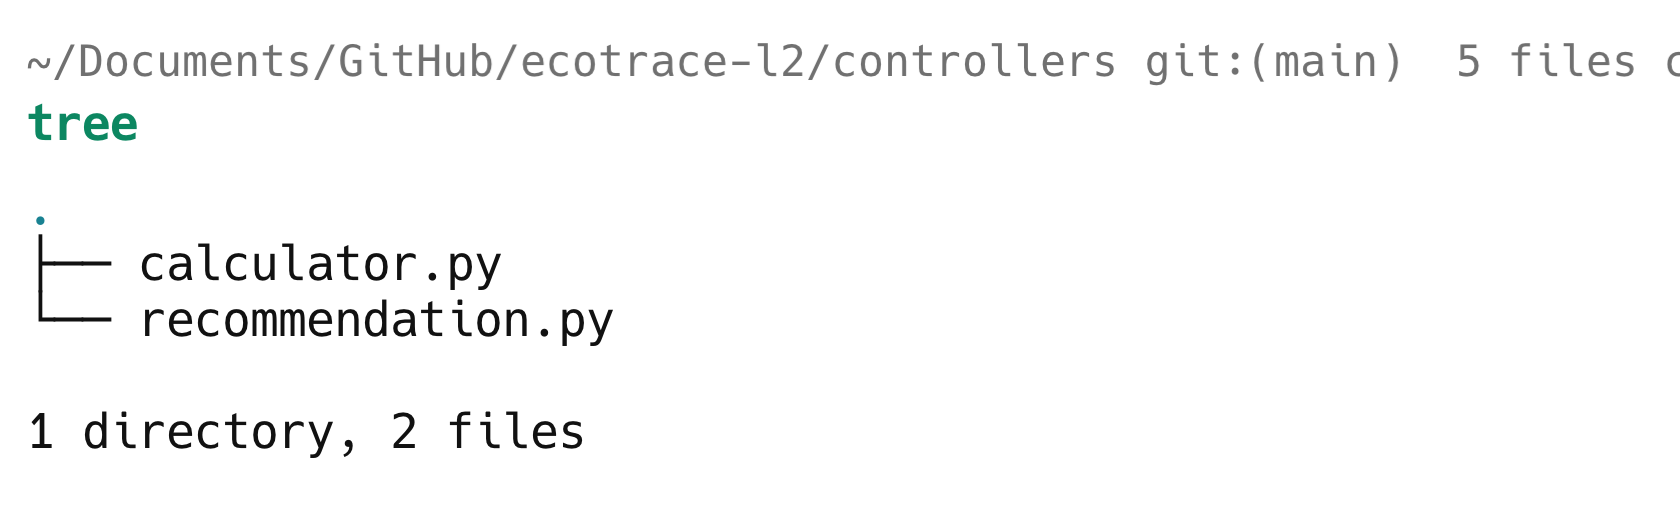
\includegraphics[width=0.7\textwidth]{captures/controllers/img1.png}
        \end{center}

        \subsection{Classe \texttt{CarbonCalculator} (\texttt{calculator.py})}
            \noindent Cette classe centralise tous les calculs relatifs à l'empreinte carbone d'un utilisateur. Voici son contenu :

            \lstinputlisting[language=Python, caption={Code du module \texttt{calculator.py} (calcul de l'empreinte carbone)}]{controllers/calculator.py}

            \noindent La classe \texttt{CarbonCalculator} est conçue pour être instanciée par utilisateur, ce qui facilite la gestion des données personnalisées :

            \begin{tcolorbox}[colback=lightgray!6, colframe=black, left=-35mm, right=5mm, top=2mm, bottom=0mm, boxrule=0.1mm]
                \begin{verbatim}
                    class CarbonCalculator:
                        def __init__(self, user_id):
                            self.user_id = user_id
                \end{verbatim}
            \end{tcolorbox}

            \noindent Les principales méthodes de cette classe sont :

            \begin{enumerate}
                \item \textbf{\texttt{calculate\_daily\_footprint}} :\\
                    Calcule l'empreinte carbone pour une journée donnée, avec gestion robuste des erreurs et répartition par catégorie (transport, alimentation, énergie, consommation).

                    \begin{tcolorbox}[colback=lightgray!6, colframe=black, left=-45mm, right=5mm, top=2mm, bottom=0mm, boxrule=0.1mm]
                        \begin{verbatim}
                            if activity.emission_factor_id is None:
                                continue
                            if emission_factor is None:
                                continue
                            if emission_factor.category not in by_category:
                                continue
                        \end{verbatim}
                    \end{tcolorbox}

                \item \textbf{\texttt{calculate\_weekly\_trend}} :\\
                    Fournit une vision temporelle sur 7 jours, avec des données formatées pour l'affichage graphique.

                    \begin{tcolorbox}[colback=lightgray!6, colframe=black, left=-45mm, right=5mm, top=2mm, bottom=0mm, boxrule=0.1mm]
                        \begin{verbatim}
                            def calculate_weekly_trend(self):
                                today = datetime.now().date()
                                start_date = today - timedelta(days=6)  # 7 jours au total
                        \end{verbatim}
                    \end{tcolorbox}

                \item \textbf{\texttt{calculate\_monthly\_summary}} :\\
                    Calcule un résumé mensuel : émissions totales, moyenne journalière, répartition par catégorie. Utilise \texttt{calendar.monthrange()} pour gérer la longueur variable des mois.

                \item \textbf{\texttt{compare\_with\_average}} :\\
                    Compare les émissions de l'utilisateur avec des moyennes nationales (valeurs de référence fixes pour le prototype, extensibles via API ou base de données).
            \end{enumerate}

        \subsection{Classe \texttt{RecommendationEngine} (\texttt{recommendation.py})}
            \noindent Cette classe gère la génération de recommandations personnalisées pour aider l'utilisateur à réduire son empreinte carbone. Voici son contenu :

            \lstinputlisting[language=Python, caption={Code du module \texttt{recommendation.py} (système de recommandations)}]{controllers/recommendation.py}

            \noindent Le système de recommandations fonctionne selon la logique suivante :

            \begin{enumerate}
                \item \textbf{Analyse des activités récentes} :\\
                    Récupère les 30 derniers jours d'activité de l'utilisateur.

                    \begin{tcolorbox}[colback=lightgray!6, colframe=black, left=-35mm, right=5mm, top=2mm, bottom=0mm, boxrule=0.1mm]
                        \begin{verbatim}
                            def get_personalized_recommendations(self):
                                # Récupérer les activités récentes (30 derniers jours)
                                recent_activities = Activity.query.filter(
                                    Activity.user_id == self.user_id,
                                    Activity.date >= start_date
                                ).all()
                        \end{verbatim}
                    \end{tcolorbox}

                \item \textbf{Fallback intelligent} :\\
                    Si l'utilisateur a moins de 5 activités, des recommandations génériques sont proposées.

                \item \textbf{Identification de la catégorie principale} :\\
                    Calcule les émissions par catégorie et cible celle qui émet le plus pour des conseils adaptés.

                \item \textbf{Gestion robuste des erreurs} :\\
                    Garantit le retour de recommandations même en cas d'erreur de données.

                    \begin{tcolorbox}[colback=lightgray!6, colframe=black, left=-45mm, right=5mm, top=2mm, bottom=0mm, boxrule=0.1mm]
                        \begin{verbatim}
                            try:
                                # Logique principale
                            except Exception as e:
                                # En cas d'erreur, retourner des recommandations génériques
                                return self._get_generic_recommendations()
                        \end{verbatim}
                    \end{tcolorbox}

                \item \textbf{Base de connaissances structurée} :\\
                    Pour chaque catégorie (transport, alimentation, énergie, consommation), une base de recommandations détaillées est disponible, incluant titre, description, impact environnemental et facilité de mise en œuvre.
            \end{enumerate}

        \subsection{Conclusion}
            \begin{tcolorbox}[colback=lightgray!6, colframe=black, left=2mm, right=5mm, top=2mm, bottom=0mm, boxrule=0.1mm]
                Le module \texttt{controllers} occupe une place centrale dans l’architecture d’EcoTrace en assurant la logique métier essentielle : calcul précis de l’empreinte carbone et génération de recommandations personnalisées. Grâce à une séparation claire des responsabilités, il garantit robustesse, évolutivité et expérience utilisateur optimale, tout en facilitant la maintenance et l’ajout de nouvelles fonctionnalités.
            \end{tcolorbox}



     % PARTIE III : LE MODULE AUTHENTIFICATION
        \newpage
        \section{PARTIE III : Le module \texttt{auth}}
            \noindent Pour gérer l'authentification des utilisateurs, le module \texttt{auth} s'appuie sur \texttt{Flask-Login} pour la gestion des sessions. Ce module est organisé de la manière suivante :

            \begin{itemize}
                \item \texttt{\_\_init\_\_.py} : Définition du module
                \item \texttt{apps.py} : Configuration du Blueprint Flask pour l'authentification
                \item \texttt{forms.py} : Formulaires de validation pour l'inscription et la connexion
                \item \texttt{models.py} : Modèle de données User avec ses méthodes principales
                \item \texttt{views.py} : Vues basées sur les classes pour gérer les requêtes HTTP
            \end{itemize}

            \noindent Cette structure permet de séparer clairement la logique métier, la validation des données et la présentation.

            \begin{center}
                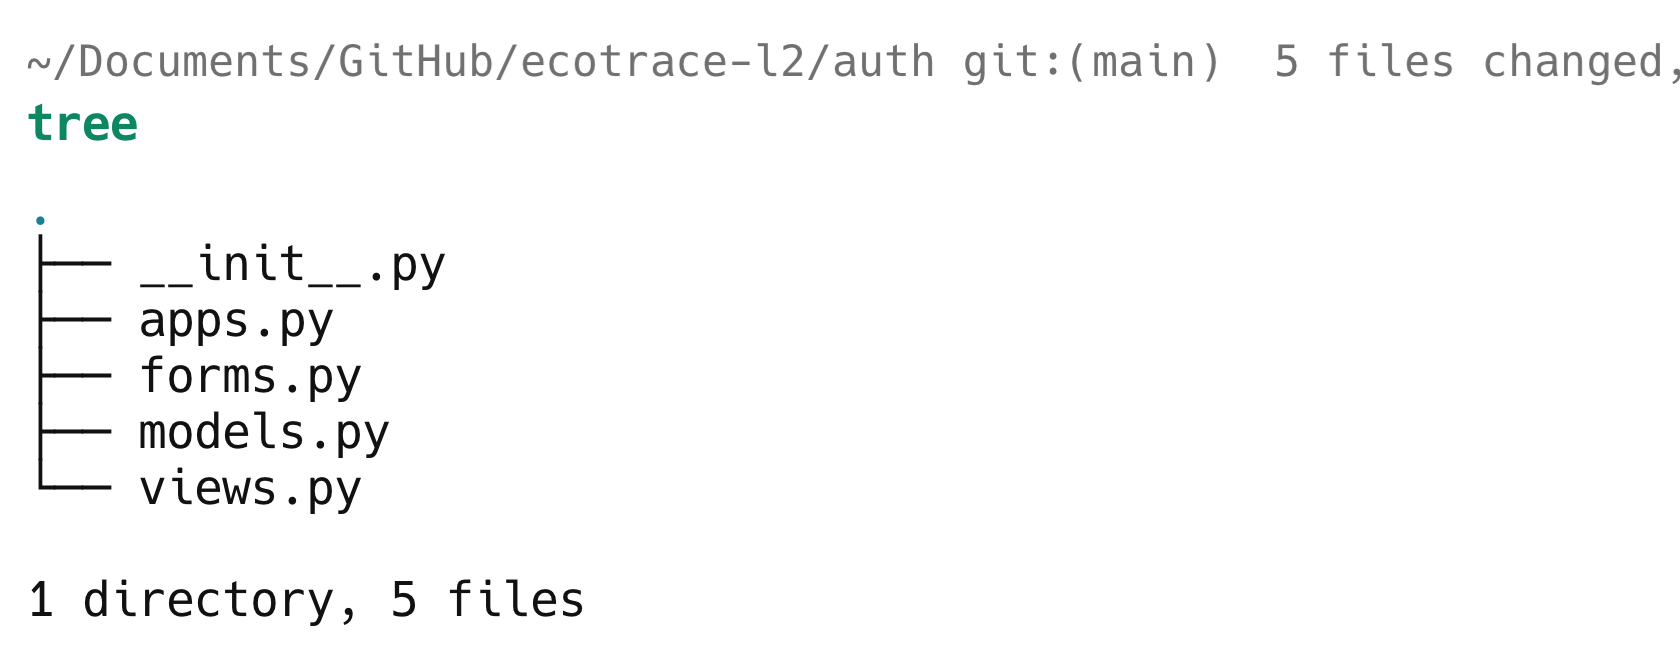
\includegraphics[width=0.7\textwidth]{captures/auth/img1.png}
            \end{center}

            \subsection{Configuration Blueprint (\texttt{apps.py})}
                \noindent Ce fichier initialise le module d'authentification en créant un Blueprint Flask et en configurant les routes associées. Voici son contenu :

                \lstinputlisting[language=Python, caption={Code du module \texttt{apps.py} (configuration du Blueprint)}]{auth/apps.py}

                \noindent Un Blueprint Flask dédié à l'authentification est créé :
                \begin{tcolorbox}[colback=lightgray!6, colframe=black, left=-35mm, right=5mm, top=2mm, bottom=0mm, boxrule=0.1mm]
                    \begin{verbatim}
                        auth = Blueprint("auth", __name__)
                    \end{verbatim}
                \end{tcolorbox}

                \noindent Quatre routes principales sont enregistrées :

                \begin{itemize}
                    \item \texttt{\/register\/} : Inscription des nouveaux utilisateurs
                    \item \texttt{\/login\/} : Connexion des utilisateurs existants
                    \item \texttt{\/logout\/} : Déconnexion
                    \item \texttt{\/dashboard\/} : Tableau de bord personnel
                \end{itemize}

                \noindent L'utilisation des vues basées sur les classes (\texttt{MethodView}) permet une meilleure organisation du code et facilite la maintenance.

            \subsection{Formulaires de validation (\texttt{forms.py})}
                \noindent Le fichier \texttt{forms.py} utilise le module \texttt{Flask-WTF} pour la conception et la validation des formulaires. Il définit les formulaires d'inscription et de connexion avec toutes les règles de validation nécessaires. Voici son contenu :

                \lstinputlisting[language=Python, caption={Code du module \texttt{forms.py} (formulaires d'authentification)}]{auth/forms.py}

                \begin{enumerate}
                    \item \textbf{RegistrationForm}:\\
                        \noindent Cette classe gère l'inscription des nouveaux utilisateurs. Elle inclut les champs suivants avec validation :

                        \begin{itemize}
                            \item Le champ nom (\texttt{name}) :
                                \begin{tcolorbox}[colback=lightgray!6, colframe=black, left=-70mm, right=5mm, top=2mm, bottom=0mm, boxrule=0.1mm]
                                    \begin{verbatim}
                                        name = StringField(
                                            'Nom', 
                                            validators=[
                                                DataRequired(message="Le nom est requis"),
                                                Length(
                                                    min=2, 
                                                    max=100, 
                                                    message="Le nom doit contenir entre 2 et 100 caractères"
                                                )
                                            ]
                                        )
                                    \end{verbatim}
                                \end{tcolorbox}
                            \item Le champ adresse mail (\texttt{email}) :
                                \begin{tcolorbox}[colback=lightgray!6, colframe=black, left=-70mm, right=5mm, top=2mm, bottom=0mm, boxrule=0.1mm]
                                    \begin{verbatim}
                                        email = StringField(
                                            'Email', 
                                            validators=[
                                                DataRequired(message="L'email est requis"),
                                                Email(message="Veuillez entrer une adresse email valide")
                                            ]
                                        )
                                    \end{verbatim}
                                \end{tcolorbox}
                            \item Le champ mot de passe (\texttt{password}) :
                                \begin{tcolorbox}[colback=lightgray!6, colframe=black, left=-75mm, right=5mm, top=2mm, bottom=0mm, boxrule=0.1mm]
                                    \begin{verbatim}
                                         password = PasswordField(
                                            'Mot de passe', 
                                            validators=[
                                                DataRequired(message="Le mot de passe est requis"),
                                                Length(
                                                    min=6, 
                                                    message="Le mot de passe doit contenir au moins 6 caractères"
                                                )
                                            ]
                                        )
                                    \end{verbatim}
                                \end{tcolorbox}
                            \item Le champ confirmation du mot de passe (\texttt{confirm\_password}) :
                                \begin{tcolorbox}[colback=lightgray!6, colframe=black, left=-75mm, right=5mm, top=2mm, bottom=0mm, boxrule=0.1mm]
                                    \begin{verbatim}
                                        confirm_password = PasswordField(
                                            'Confirmer le mot de passe', 
                                            validators=[
                                                DataRequired(message="La confirmation du mot de passe est requise"),
                                                EqualTo(
                                                    'password', 
                                                    message="Les mots de passe ne correspondent pas"
                                                )
                                            ]
                                        )
                                    \end{verbatim}
                                \end{tcolorbox}
                        \end{itemize}

                        \noindent Pour empêcher la création de comptes avec des emails déjà utilisés, une validation personnalisée est ajoutée dans la méthode \texttt{validate\_email} :
                        \begin{tcolorbox}[colback=lightgray!6, colframe=black, left=-45mm, right=5mm, top=2mm, bottom=0mm, boxrule=0.1mm]
                            \begin{verbatim}
                                def validate_email(self, email):
                                    user = User.query.filter_by(email=email.data).first()
                                    if user:
                                        raise ValidationError("Cette adresse email est déjà utilisée")
                            \end{verbatim}
                        \end{tcolorbox}

                    \item \textbf{LoginForm}:\\
                        \noindent Cette classe gère la connexion des utilisateurs existants. Elle inclut les champs suivants :
                        \begin{enumerate}
                            \item Le champ adresse mail (\texttt{email}) qui sert à identifier l'utilisateur.
                            \item Le champ mot de passe (\texttt{password})
                            \item La case à cocher "Se souvenir de moi" (\texttt{remember}) qui permet de garder l'utilisateur connecté.
                        \end{enumerate}
                \end{enumerate}

            \subsection{Modèle User (\texttt{models.py})}
                \noindent Le fichier \texttt{models.py} définit le modèle de données \texttt{User} qui représente les utilisateurs de l'application. Il hérite de \texttt{db.Model} de \texttt{Flask-SQLAlchemy} et de \texttt{UserMixin} pour bénéficier des fonctionnalités de \texttt{Flask-Login}. Voici son contenu :

                \lstinputlisting[language=Python, caption={Code du module \texttt{models.py} (modèle User)}]{auth/models.py}

                \begin{enumerate}
                    \item \textbf{Sécurité des mots de passe}:\\
                        \noindent Le module \texttt{werkzeug.security} est utilisé pour hacher les mots de passe avant de les stocker dans la base de données :
                        \begin{tcolorbox}[colback=lightgray!6, colframe=black, left=-45mm, right=5mm, top=2mm, bottom=0mm, boxrule=0.1mm]
                            \begin{verbatim}
                                def __init__(self, name, email, password):
                                    self.password = generate_password_hash(password)
                            \end{verbatim}
                        \end{tcolorbox}
                    
                        \noindent Une méthode permet également de vérifier les mots de passe lors de la connexion :
                        \begin{tcolorbox}[colback=lightgray!6, colframe=black, left=-45mm, right=5mm, top=2mm, bottom=0mm, boxrule=0.1mm]
                            \begin{verbatim}
                                def check_password(self, password2):
                                    return check_password_hash(self.password, password2)
                            \end{verbatim}
                        \end{tcolorbox}

                    \item \textbf{Relations avec les données carbone}:\\
                        \noindent Une relation est établie avec le modèle \texttt{Activity} :
                        \begin{tcolorbox}[colback=lightgray!6, colframe=black, left=-45mm, right=5mm, top=2mm, bottom=0mm, boxrule=0.1mm]
                            \begin{verbatim}
                                activities = db.relationship('Activity', backref='user', lazy=True)
                            \end{verbatim}
                        \end{tcolorbox}

                        \noindent Cette relation permet d'accéder facilement à toutes les activités d'un utilisateur.

                    \item \textbf{Méthodes de calcul personnalisées}:\\
                        \noindent 
                        \begin{enumerate}
                            \item \underline{Calcul des émissions personnelles} :
                                \begin{tcolorbox}[colback=lightgray!6, colframe=black, left=-70mm, right=5mm, top=2mm, bottom=0mm, boxrule=0.1mm]
                                    \begin{verbatim}
                                        def get_total_emissions(self):
                                            total = 0
                                            for activity in self.activities:
                                                factor = EmissionFactor.query.get(activity.emission_factor_id)
                                                total += activity.quantity * factor.co2_factor
                                            return total
                                    \end{verbatim}
                                \end{tcolorbox}

                            \item \underline{Méthodes de classe pour les statistiques globales} :
                                \noindent Des méthodes de classe fournissent des données à l'ensemble de l'application :
                                \begin{itemize}
                                    \item \texttt{get\_all\_users\_total\_emissions()} : Calcule et formate les émissions totales de tous les utilisateurs
                                    \item \texttt{get\_total\_users()} : Retourne le nombre d'utilisateurs avec formatage optionnel
                                \end{itemize}
                        \end{enumerate}

                    \noindent Le formatage automatique des unités est particulièrement utile :
                    
                    \begin{tcolorbox}[colback=lightgray!6, colframe=black, left=-45mm, right=5mm, top=2mm, bottom=0mm, boxrule=0.1mm]
                        \begin{verbatim}
                            if total >= 1_000_000:
                                return f"{round(total/1_000_000, 2)} MtCO2"
                            elif total >= 1_000:
                                return f"{round(total/1_000, 2)} ktCO2"
                        \end{verbatim}
                    \end{tcolorbox}
                \end{enumerate}

            \subsection{Vues d'authentification (\texttt{views.py})}
                \noindent Le fichier \texttt{views.py} contient les vues basées sur les classes pour gérer les requêtes HTTP liées à l'authentification. Voici son contenu :

                \lstinputlisting[language=Python, caption={Code du module \texttt{views.py} (vues d'authentification)}]{auth/views.py}

                \begin{enumerate}
                    \item \textbf{Inscription (\texttt{RegisterView})}:\\
                        \noindent Gère l'inscription des nouveaux utilisateurs à l'aide du formulaire \texttt{RegistrationForm}. En cas de succès, l'utilisateur est redirigé vers la page de connexion.

                        \noindent Cette vue inclut une gestion complète :

                        \begin{itemize}
                            \item \underline{Gestion des utilisateurs déjà connectés} : Redirige les utilisateurs déjà connectés vers le tableau de bord s'ils tentent d'accéder à la page d'inscription.

                            \begin{tcolorbox}[colback=lightgray!6, colframe=black, left=-60mm, right=5mm, top=2mm, bottom=0mm, boxrule=0.1mm]
                                \begin{verbatim}
                                    if current_user.is_authenticated:
                                        flash("Vous êtes déjà connecté.", "info")
                                        return redirect(url_for('auth.dashboard'))
                                \end{verbatim}
                            \end{tcolorbox}

                            \item \underline{Vérification de l'unicité de l'email} : Vérifie si l'email fourni par l'utilisateur est déjà utilisé. Si c'est le cas, un message d'erreur est affiché.

                            \begin{tcolorbox}[colback=lightgray!6, colframe=black, left=-60mm, right=5mm, top=2mm, bottom=0mm, boxrule=0.1mm]
                                \begin{verbatim}
                                    existing_user = User.query.filter_by(email=email).first()
                                    if existing_user:
                                        flash("Un utilisateur avec cet email existe déjà.", "error")
                                        return redirect(url_for('auth.register'))
                                \end{verbatim}
                            \end{tcolorbox}
                        \end{itemize}

                    \item \textbf{Connexion (\texttt{LoginView})}:\\
                        \noindent Gère la connexion des utilisateurs existants à l'aide du formulaire \texttt{LoginForm}. En cas de succès, l'utilisateur est redirigé vers le tableau de bord.

                        \noindent Cette vue inclut :

                        \begin{itemize}
                            \item \underline{Authentification sécurisée} : Utilise \texttt{Flask-Login} pour vérifier les identifiants et gérer la session utilisateur.

                                \begin{tcolorbox}[colback=lightgray!6, colframe=black, left=-60mm, right=5mm, top=2mm, bottom=0mm, boxrule=0.1mm]
                                    \begin{verbatim}
                                        if user and user.check_password(form.password.data):
                                            login_user(user, remember=form.remember.data)
                                    \end{verbatim}
                                \end{tcolorbox}

                            \item \underline{Redirection intelligente} : Utilise la variable \texttt{next} pour rediriger l'utilisateur vers la page qu'il souhaitait atteindre avant de se connecter ou vers le tableau de bord par défaut.

                                \begin{tcolorbox}[colback=lightgray!6, colframe=black, left=-60mm, right=5mm, top=2mm, bottom=0mm, boxrule=0.1mm]
                                    \begin{verbatim}
                                        next_page = request.args.get('next')
                                        return redirect(next_page or url_for('auth.dashboard'))
                                    \end{verbatim}
                                \end{tcolorbox}
                        \end{itemize}

                    \item \textbf{Déconnexion (\texttt{LogoutView})}:\\
                        \noindent Gère la déconnexion des utilisateurs en appelant la méthode \texttt{logout\_user()} de \texttt{Flask-Login}.

                    \item \textbf{Tableau de bord (\texttt{DashboardView})}:\\
                        \noindent Affiche les statistiques personnelles de l'utilisateur : empreinte carbone quotidienne, hebdomadaire et mensuelle, ainsi que les recommandations personnalisées.

                        \noindent Cette vue intègre :

                        \begin{itemize}
                            \item \underline{Sécurité} : 
                                \begin{tcolorbox}[colback=lightgray!6, colframe=black, left=-60mm, right=5mm, top=2mm, bottom=0mm, boxrule=0.1mm]
                                    \begin{verbatim}
                                        decorators = [login_required]
                                    \end{verbatim}
                                \end{tcolorbox}
                            \item \underline{Gestion robuste des erreurs} : Chaque calcul est enveloppé dans des blocs \texttt{try/except} pour éviter que l'application ne plante en cas de données corrompues.
                                \begin{tcolorbox}[colback=lightgray!6, colframe=black, left=-60mm, right=5mm, top=2mm, bottom=0mm, boxrule=0.1mm]
                                    \begin{verbatim}
                                        try:
                                            # Code qui pourrait lever une exception
                                        except Exception as e:
                                            # Gestion de l'exception
                                    \end{verbatim}
                                \end{tcolorbox}
                            \item \underline{Intégration des contrôleurs} : Les classes du module controllers sont utilisées pour fournir des données riches au tableau de bord.
                                \begin{tcolorbox}[colback=lightgray!6, colframe=black, left=-60mm, right=5mm, top=2mm, bottom=0mm, boxrule=0.1mm]
                                    \begin{verbatim}
                                        calculator = CarbonCalculator(user_id)
                                        recommendation_engine = RecommendationEngine(user_id)
                                    \end{verbatim}
                                \end{tcolorbox}
                            \item \underline{Préparation des données JavaScript} : Les données sont préparées au format JSON pour permettre l'affichage de graphiques interactifs côté client.
                                \begin{tcolorbox}[colback=lightgray!6, colframe=black, left=-60mm, right=5mm, top=2mm, bottom=0mm, boxrule=0.1mm]
                                    \begin{verbatim}
                                        weekly_trend_json = json.dumps(weekly_trend)
                                        categories_json = json.dumps(daily_footprint['by_category'])
                                    \end{verbatim}
                                \end{tcolorbox}
                        \end{itemize}
                \end{enumerate}

                \noindent Le module \texttt{auth} fournit ainsi une base d'authentification solide et sécurisée, essentielle pour protéger les données personnelles des utilisateurs d'EcoTrace.


            \subsection{Conclusion}
                \begin{tcolorbox}[colback=lightgray!6, colframe=black, left=2mm, right=5mm, top=2mm, bottom=0mm, boxrule=0.1mm]
                    En conclusion, le module \texttt{auth} d'EcoTrace joue un rôle central dans la protection des données des utilisateurs. Grâce à une authentification robuste et à une gestion sécurisée des sessions, seules les personnes autorisées ont accès aux informations sensibles. L'intégration du hachage des mots de passe et de la vérification de l'e-mail renforce encore la sécurité globale de l'application.
                \end{tcolorbox}


    % PARTIE IV: LE MODULE CARBON
        \newpage
        \section{PARTIE IV : Le module \texttt{carbon}}
            \noindent Le module \texttt{carbon} gère le coeur fonctionnel de l'application, à savoir le suivi des émissions carbone. Il reprend la même architecture que le module \texttt{auth}, assurant ainsi la cohérence et la clarté de l'organisation du projet :

            \begin{itemize}
                \item \texttt{\_\_init\_\_.py} : Initialisation du module
                \item \texttt{apps.py} : Configuration du Blueprint pour les fonctionnalités carbone
                \item \texttt{forms.py} : Formulaire pour l'ajout d'activités
                \item \texttt{models.py} : Modèles EmissionFactor et Activity
                \item \texttt{views.py} : Vues pour la gestion des activités carbone
            \end{itemize}

            \noindent Cette structure garantit une séparation claire des responsabilités et une maintenance facilitée.

            \begin{center}
                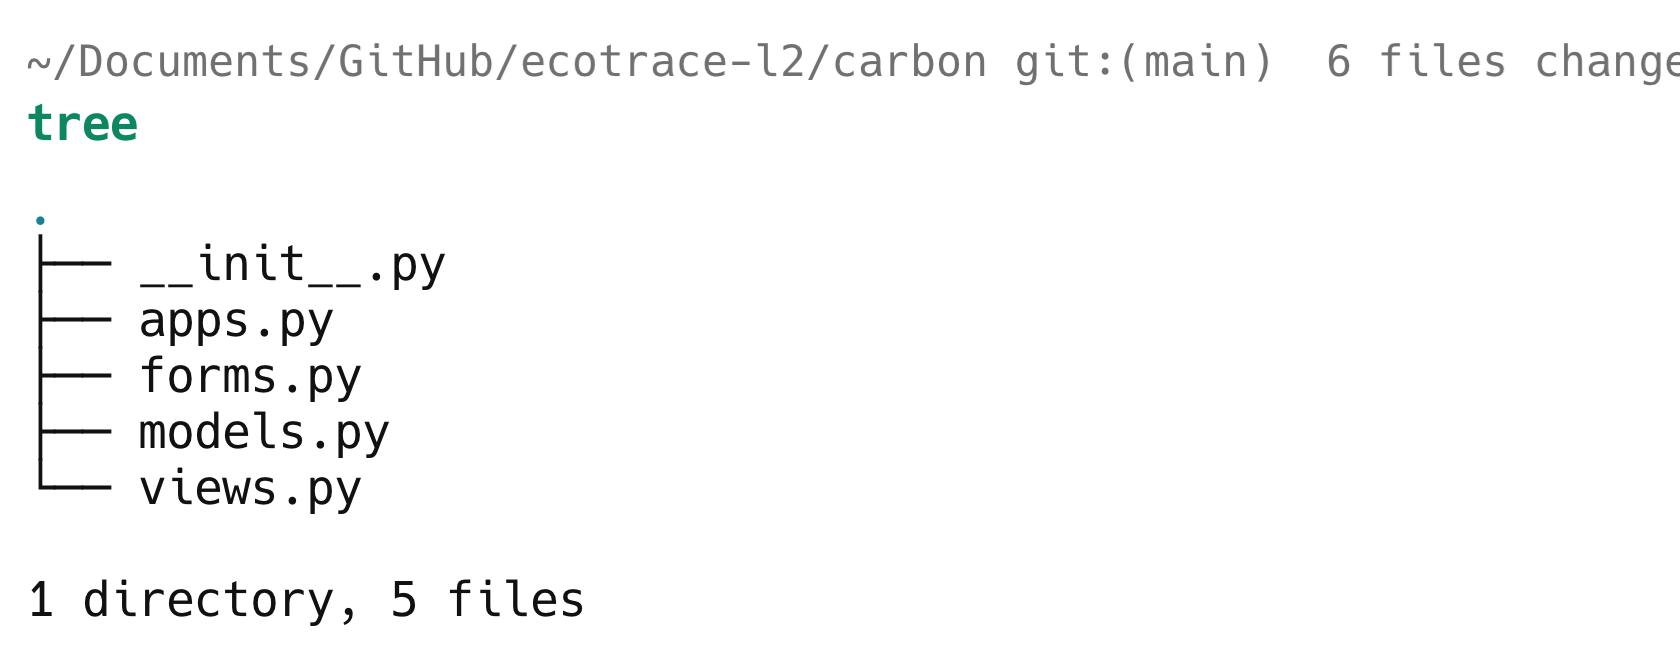
\includegraphics[width=0.7\textwidth]{captures/carbon/img1.png}
            \end{center}

            \subsection{Configuration Blueprint (\texttt{apps.py})}
                \noindent Le Blueprint \texttt{carbon} propose quatre routes principales :

                \begin{tcolorbox}[colback=lightgray!6, colframe=black, left=-35mm, right=5mm, top=2mm, bottom=0mm, boxrule=0.1mm]
                    \begin{verbatim}
                        carbon = Blueprint("carbon", __name__)
                    \end{verbatim}
                \end{tcolorbox}

                \noindent Les routes définies sont :

                \begin{itemize}
                    \item \texttt{/} : Page d'accueil de l'application
                    \item \texttt{/add\_activity/} : Formulaire d'ajout d'activité
                    \item \texttt{/history/} : Historique des activités de l'utilisateur
                    \item \texttt{/activity/delete/<int:activity\_id>/} : Suppression d'une activité spécifique
                \end{itemize}

                \noindent L'utilisation d'une route paramétrique pour la suppression permet une gestion sécurisée et personnalisée des activités.

            \subsection{Formulaire d'ajout d'activité \texttt{AddActivityForm} (\texttt{forms.py})}
                \noindent Le fichier \texttt{forms.py} contient le formulaire d'ajout d'activité, qui permet à l'utilisateur de saisir ses activités quotidiennes. Voici son contenu :

                \lstinputlisting[language=Python, caption={Code du module \texttt{forms.py} (formulaire d'ajout d'activité)}]{carbon/forms.py}

                \noindent Ce formulaire comprend les champs suivants :

                \begin{itemize}
                    \item \texttt{category} : Catégorie de l'activité (transport, alimentation, etc.)
                    \item \texttt{activity\_id} : Identifiant de l'activité
                    \item \texttt{quantity} : Quantité d'émissions (en kgCO2)
                    \item \texttt{date} : Date de l'activité
                \end{itemize}

                \noindent Le formulaire est conçu pour être convivial et intuitif, facilitant la saisie des données par l'utilisateur. Il propose notamment :

                \begin{enumerate}
                    \item \textbf{Sélection de la catégorie} : L'utilisateur choisit la catégorie de l'activité (transport, alimentation, etc.) via une liste déroulante.
                    \begin{tcolorbox}[colback=lightgray!6, colframe=black, left=-45mm, right=5mm, top=2mm, bottom=0mm, boxrule=0.1mm]
                        \begin{verbatim}
                            category = SelectField(
                                label="Catégorie",
                                choices=[
                                    ("", "Sélectionnez une catégorie"),
                                    ("transport", "Transport"),
                                    ("food", "Alimentation"),
                                    ("energy", "Énergie"),
                                    ("consumption", "Consommation"),
                                ],
                                validators=[DataRequired(message="Le champ catégorie est requis")],
                            )
                        \end{verbatim}
                    \end{tcolorbox}

                    \item \textbf{Champ d'activité dynamique} : Le champ d'activité s'adapte en fonction de la catégorie sélectionnée. Par exemple, si l'utilisateur choisit "Transport", les options proposées seront spécifiques à cette catégorie.

                    \begin{tcolorbox}[colback=lightgray!6, colframe=black, left=-45mm, right=5mm, top=2mm, bottom=0mm, boxrule=0.1mm]
                        \begin{verbatim}
                            activity_id = SelectField(
                                label="Type d'activité",
                                choices=[],  // Les choix sont remplis dynamiquement
                                validators=[Optional()],
                            )
                        \end{verbatim}
                    \end{tcolorbox}

                    \noindent Cette approche permet de charger dynamiquement les activités disponibles selon la catégorie sélectionnée.

                    \item \textbf{Validation numérique} : Le champ \texttt{quantity} est validé pour garantir une valeur numérique positive, représentant la quantité d'émissions en kgCO2.
                    \begin{tcolorbox}[colback=lightgray!6, colframe=black, left=-45mm, right=5mm, top=2mm, bottom=0mm, boxrule=0.1mm]
                        \begin{verbatim}
                            quantity = FloatField(
                                validators=[
                                    DataRequired(message="Le champ quantité est requis"),
                                    NumberRange(min=0, message="La quantité doit être positive"),
                                ],
                            )
                        \end{verbatim}
                    \end{tcolorbox}
                \end{enumerate}

            \subsection{Modèles de données (\texttt{models.py})}
                \noindent Le fichier \texttt{models.py} contient les modèles de données pour les facteurs d'émission et les activités. Voici son contenu :

                \lstinputlisting[language=Python, caption={Code du module \texttt{models.py} (modèles de données)}]{carbon/models.py}

                \begin{enumerate}
                    \item \textbf{Modèle EmissionFactor} :\\
                        Ce modèle représente les facteurs d'émission pour différentes activités. Il comprend les champs suivants :

                        \begin{tcolorbox}[colback=lightgray!6, colframe=black, left=-45mm, right=5mm, top=2mm, bottom=0mm, boxrule=0.1mm]
                            \begin{verbatim}
                                class EmissionFactor(db.Model):
                                    __tablename__ = 'emission_factors'
                                    
                                    id = db.Column(db.Integer, primary_key=True)
                                    category = db.Column(db.String(50), nullable=False)
                                    subcategory = db.Column(db.String(50), nullable=False)
                                    activity_name = db.Column(db.String(100), nullable=False)
                                    unit = db.Column(db.String(20), nullable=False)
                                    co2_factor = db.Column(db.Float, nullable=False)
                                    source = db.Column(db.String(100))
                            \end{verbatim}
                        \end{tcolorbox}

                        \begin{itemize}
                            \item \texttt{id} : Identifiant unique
                            \item \texttt{category} : Catégorie de l'activité
                            \item \texttt{subcategory} : Sous-catégorie de l'activité
                            \item \texttt{activity\_name} : Nom de l'activité
                            \item \texttt{unit} : Unité de mesure
                            \item \texttt{co2\_factor} : Facteur d'émission en kgCO2 par unité
                            \item \texttt{source} : Source du facteur d'émission (ADEME)
                        \end{itemize}

                        \noindent Cette structure permet de constituer une base de données complète avec les données de l'\href{https://www.ademe.fr/}{ADEME} intégrées dans \texttt{settings.py}.

                        \noindent Une méthode de classe utile, \texttt{get\_by\_category}, permet de récupérer les facteurs d'émission par catégorie :

                        \begin{tcolorbox}[colback=lightgray!6, colframe=black, left=-45mm, right=5mm, top=2mm, bottom=0mm, boxrule=0.1mm]
                            \begin{verbatim}
                                @classmethod
                                def get_by_category(cls, category):
                                    return cls.query.filter_by(category=category).all()
                            \end{verbatim}
                        \end{tcolorbox}

                    \item \textbf{Modèle Activity} :\\
                        Ce modèle représente une activité effectuée par l'utilisateur. Il comprend les champs suivants :

                        \begin{tcolorbox}[colback=lightgray!6, colframe=black, left=-55mm, right=5mm, top=2mm, bottom=0mm, boxrule=0.1mm]
                            \begin{verbatim}
                                class Activity(db.Model):
                                    __tablename__ = 'activities'
                                    
                                    id = db.Column(db.Integer, primary_key=True)
                                    user_id = db.Column(db.Integer, db.ForeignKey('users.id'), nullable=False)
                                    emission_factor_id = db.Column(
                                        db.Integer, 
                                        db.ForeignKey('emission_factors.id'), nullable=False
                                    )
                                    quantity = db.Column(db.Float, nullable=False)
                                    date = db.Column(
                                        db.Date, 
                                        nullable=False, 
                                        default=datetime.now(timezone.utc).date()
                                    )
                            \end{verbatim}
                        \end{tcolorbox}

                        \begin{itemize}
                            \item \texttt{id} : Identifiant unique
                            \item \texttt{user\_id} : Identifiant de l'utilisateur (clé étrangère)
                            \item \texttt{emission\_factor\_id} : Identifiant du facteur d'émission associé
                            \item \texttt{quantity} : Quantité d'émissions en kgCO2
                            \item \texttt{date} : Date de l'activité
                        \end{itemize}

                        \noindent Quelques méthodes utiles :

                        \begin{tcolorbox}[colback=lightgray!6, colframe=black, left=-45mm, right=5mm, top=2mm, bottom=0mm, boxrule=0.1mm]
                            \begin{verbatim}
                                def get_emissions(self):
                                    factor = EmissionFactor.query.get(self.emission_factor_id)
                                    return self.quantity * factor.co2_factor
                            \end{verbatim}
                        \end{tcolorbox}

                        \noindent Cette méthode permet de calculer facilement les émissions d'une activité.

                        \noindent Une méthode de classe permet également le formatage dynamique des statistiques :

                        \begin{tcolorbox}[colback=lightgray!6, colframe=black, left=-45mm, right=5mm, top=2mm, bottom=0mm, boxrule=0.1mm]
                            \begin{verbatim}
                                @classmethod
                                def get_total_activities(cls):
                                    count = cls.query.count()
                                    if count < 1000:
                                        return str(count)
                                    elif count < 1_000_000:
                                        return f"{count/1000:.1f}K".rstrip('0').rstrip('.')
                                    else:
                                        return f"{count/1_000_000:.1f}M".rstrip('0').rstrip('.')
                            \end{verbatim}
                        \end{tcolorbox}
                \end{enumerate}

            \subsection{Vues de gestion des activités (\texttt{views.py})}
                \noindent Le fichier \texttt{views.py} contient les vues pour gérer les activités carbone. Voici son contenu :

                \lstinputlisting[language=Python, caption={Code du module \texttt{views.py} (vues de gestion des activités)}]{carbon/views.py}

                \begin{enumerate}
                    \item \textbf{Page d'accueil (\texttt{IndexView})} :\\
                        Vue simple pour la page d'accueil, point d'entrée de l'application, affichant les statistiques globales (injectées par les processeurs de contexte).

                    \item \textbf{Ajout d'activité (\texttt{AddActivityView})} :\\
                        Gère le formulaire d'ajout d'activité. En cas de succès, l'utilisateur est redirigé vers la même page pour faciliter l'ajout de plusieurs activités. Cette vue intègre plusieurs innovations :

                        \begin{itemize}
                            \item \underline{Optimisation avec cache} :
                                \begin{tcolorbox}[colback=lightgray!6, colframe=black, left=-70mm, right=5mm, top=2mm, bottom=0mm, boxrule=0.1mm]
                                    \begin{verbatim}
                                        @lru_cache(maxsize=128)
                                        def _get_emission_factors(self):
                                            return {
                                                category: EmissionFactor.query.filter_by(category=category).all()
                                                for category in self.VALID_CATEGORIES
                                            }
                                    \end{verbatim}
                                \end{tcolorbox}
                                \noindent L'utilisation de \texttt{lru\_cache} évite de solliciter la base de données à chaque affichage du formulaire.

                            \item \underline{Validation centralisée} : Une méthode dédiée valide toutes les données et retourne à la fois les erreurs et les données validées.
                            
                                \begin{tcolorbox}[colback=lightgray!6, colframe=black, left=-60mm, right=5mm, top=2mm, bottom=0mm, boxrule=0.1mm]
                                    \begin{verbatim}
                                        def _validate_form_data(self, form_data):
                                            errors = []
                                            validated_data = {}
                                            
                                            // Validation catégorie
                                            category = form_data.get("category", "").strip()
                                            if not category:
                                                errors.append("Veuillez sélectionner une catégorie.")
                                            elif category not in self.VALID_CATEGORIES:
                                                errors.append(f"Catégorie '{category}' non valide.")
                                    \end{verbatim}
                                \end{tcolorbox}

                            \item \underline{Gestion d'erreurs robuste} : Un système de rollback automatique est utilisé en cas d'erreur lors de la création.
                            
                                \begin{tcolorbox}[colback=lightgray!6, colframe=black, left=-70mm, right=5mm, top=2mm, bottom=0mm, boxrule=0.1mm]
                                    \begin{verbatim}
                                        def _create_activity(self, validated_data):
                                            try:
                                                activity = Activity(...)
                                                db.session.add(activity)
                                                db.session.commit()
                                                return True
                                            except Exception as e:
                                                db.session.rollback()
                                                flash(
                                                    "Une erreur s'est produite lors de l'ajout de l'activité.", 
                                                    "danger"
                                                )
                                                return False
                                    \end{verbatim}
                                \end{tcolorbox}
                        \end{itemize}

                    \item \textbf{Historique des activités (\texttt{ActivityHistoryView})} :\\
                        Cette vue affiche l'historique des activités de l'utilisateur, offrant un aperçu des actions passées et la possibilité de les gérer.

                        \noindent Elle inclut :

                        \begin{itemize}
                            \item \underline{Requête optimisée} :
                                \begin{tcolorbox}[colback=lightgray!6, colframe=black, left=-60mm, right=5mm, top=2mm, bottom=0mm, boxrule=0.1mm]
                                    \begin{verbatim}
                                        activities = (
                                            Activity.query
                                            .filter_by(user_id=current_user.id)
                                            .order_by(Activity.date.desc())
                                            .all()
                                        )
                                    \end{verbatim}
                                \end{tcolorbox}

                            \item \underline{Préparation des données pour JavaScript} : Les données sont formatées pour permettre l'affichage de graphiques côté client.

                                \begin{tcolorbox}[colback=lightgray!6, colframe=black, left=-60mm, right=5mm, top=2mm, bottom=0mm, boxrule=0.1mm]
                                    \begin{verbatim}
                                        for activity in activities:
                                            emission_factor = EmissionFactor.query.get(
                                                activity.emission_factor_id
                                            )
                                            activities_data.append({
                                                'id': activity.id,
                                                'date': activity.date,
                                                'category': emission_factor.category,
                                                'name': emission_factor.activity_name,
                                                'quantity': activity.quantity,
                                                'unit': emission_factor.unit,
                                                'emissions': round(
                                                    activity.quantity * emission_factor.co2_factor,
                                                    2
                                                )
                                            })
                                    \end{verbatim}
                                \end{tcolorbox}
                        \end{itemize}

                    \item \textbf{Suppression d'activité (\texttt{DeleteActivityView})} :\\
                        Gère la suppression sécurisée d'une activité spécifique selon son identifiant.

                        \begin{tcolorbox}[colback=lightgray!6, colframe=black, left=-60mm, right=5mm, top=2mm, bottom=0mm, boxrule=0.1mm]
                            \begin{verbatim}
                                activity = Activity.query.filter_by(
                                    id=activity_id, 
                                    user_id=user.id
                                ).first()

                                if not activity:
                                    flash(
                                        "Activité non trouvée ou vous n'avez pas la permission de la supprimer.", 
                                        "danger"
                                    )
                                    return redirect(url_for("carbon.history"))
                            \end{verbatim}
                        \end{tcolorbox}

                        \noindent Cette vérification empêche un utilisateur de supprimer les activités d'autres utilisateurs.

                        \noindent L'utilisateur est redirigé vers la page précédente, avec un fallback vers l'historique si besoin.

                        \begin{tcolorbox}[colback=lightgray!6, colframe=black, left=-50mm, right=5mm, top=2mm, bottom=0mm, boxrule=0.1mm]
                            \begin{verbatim}
                                return redirect(request.referrer) or redirect(url_for("carbon.history"))
                            \end{verbatim}
                        \end{tcolorbox}
                \end{enumerate}

                \noindent Les vues (\texttt{AddActivityView}, \texttt{HistoryView}, \texttt{DeleteActivityView}) sont protégées par le décorateur \texttt{@login\_required}, garantissant que seuls les utilisateurs authentifiés peuvent y accéder.

                \noindent Le module \texttt{carbon} constitue le coeur fonctionnel d'EcoTrace et illustre une approche professionnelle du développement web avec Flask.

            \subsection{Conclusion}
                \begin{tcolorbox}[colback=lightgray!6, colframe=black, left=2mm, right=5mm, top=2mm, bottom=0mm, boxrule=0.1mm]
                    En résumé, le module \texttt{carbon} d'EcoTrace permet aux utilisateurs de suivre et de gérer leurs émissions de carbone de manière efficace. Grâce à une architecture modulaire et à des vues sécurisées, ils peuvent facilement ajouter, visualiser et supprimer leurs activités tout en bénéficiant d'une expérience utilisateur cohérente et fluide.
                \end{tcolorbox}


    % PARTIE V: LES TEMPLATES ET STATIQUES
        \newpage
        \section{PARTIE V: Les templates et fichiers statiques}
            \noindent Pour créer une interface utilisateur moderne et cohérente, j'ai utilisé le moteur de rendu \href{https://jinja.palletsprojects.com/}{Jinja2} et le framework CSS \href{https://tailwindcss.com/}{TailwindCSS}. Les templates sont organisés selon une architecture hiérarchique :

                \begin{tcolorbox}[colback=lightgray!6, colframe=black, left=-35mm, right=5mm, top=2mm, bottom=0mm, boxrule=0.1mm]
                    \begin{verbatim}
                        assets/templates/
                        ├── auth/                   # Templates d'authentification
                        │   ├── dashboard.html
                        │   ├── login.html
                        │   └── register.html
                        ├── carbon/                 # Templates fonctionnels
                        │   ├── add_activity.html
                        │   ├── history.html
                        │   └── index.html
                        ├── errors/                 # Pages d'erreur
                        │   ├── 404.html
                        │   └── 500.html
                        └── partials/              # Composants réutilisables
                            ├── base.html
                            ├── footer.html
                            └── navbar.html
                    \end{verbatim}
                \end{tcolorbox}

                \noindent Cette organisation garantit une cohérence visuelle et facilite la maintenance et l'évolution du projet.

                \noindent Je n'inclus pas ici l'intégralité du code des templates pour des raisons de place ; ils sont disponibles dans le répertoire dédié. Je propose ci-dessous une explication structurée.

            \bigskip
            \textbf{LES TEMPLATES}\\\\
            \noindent Les templates sont des fichiers HTML qui définissent la structure et le contenu des pages web. Ils utilisent le moteur de templates Jinja2 pour intégrer des données dynamiques et faciliter la réutilisation du code.

            \begin{center}
                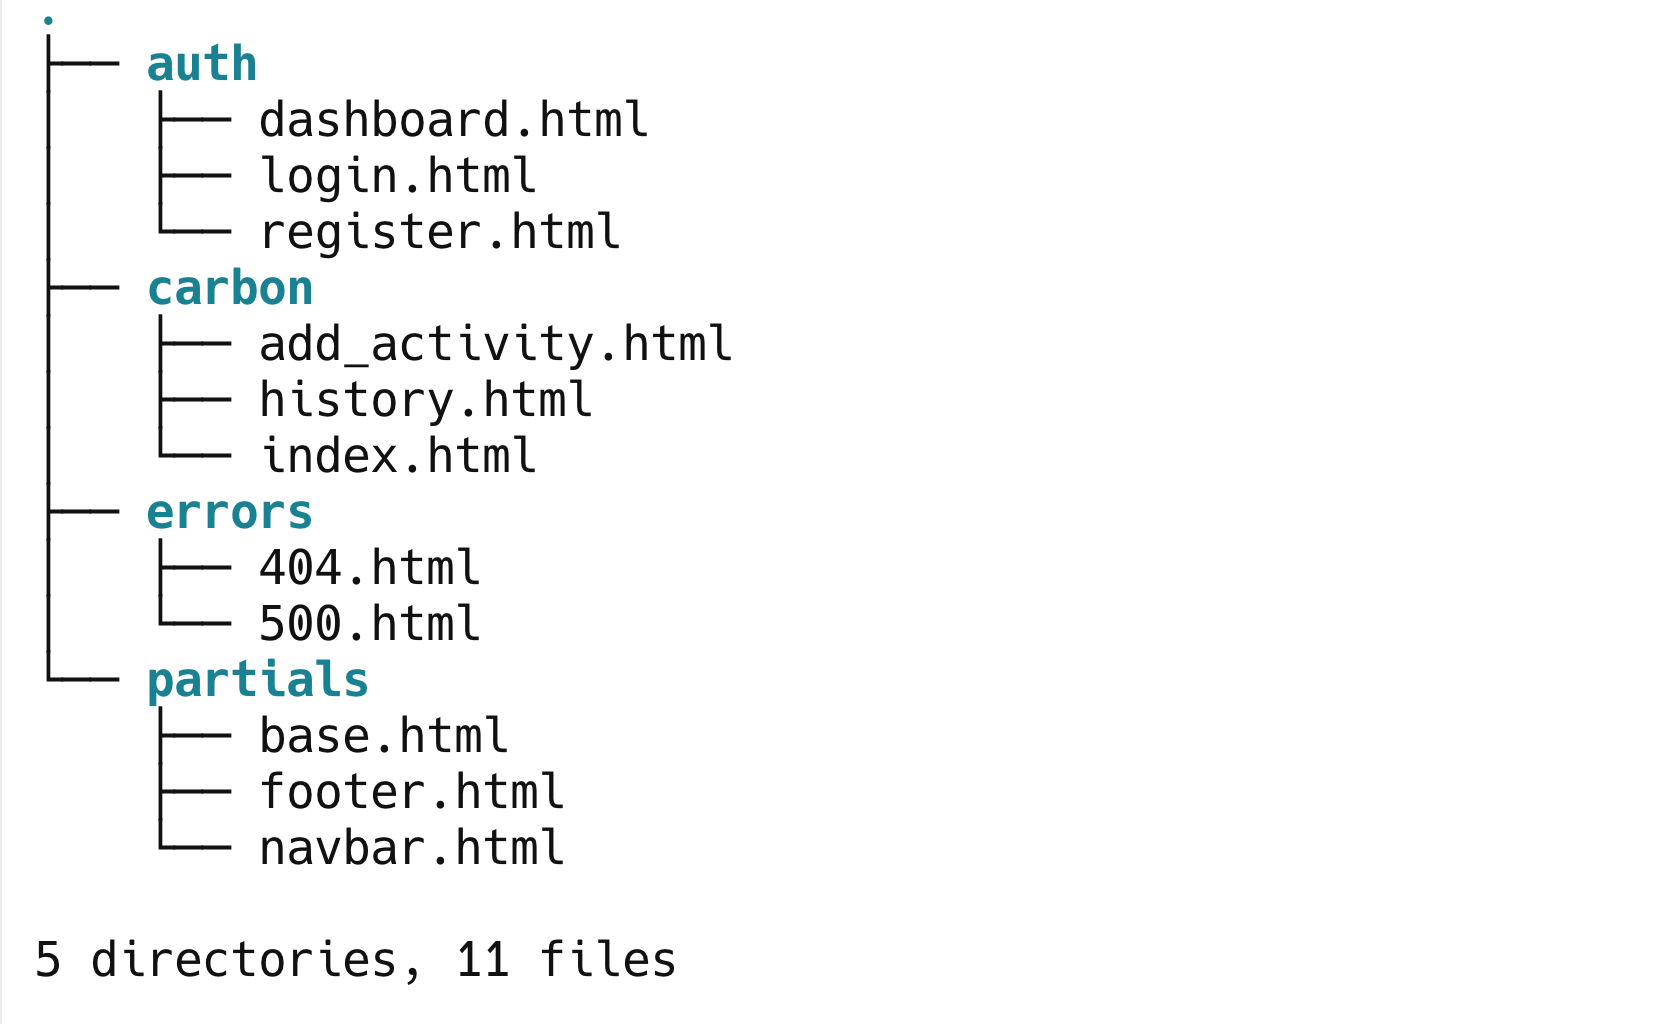
\includegraphics[width=0.7\textwidth]{captures/templates_et_static/img1.png}
            \end{center}

            \subsection{Les templates partiels (\texttt{partials/})}
                \begin{center}
                    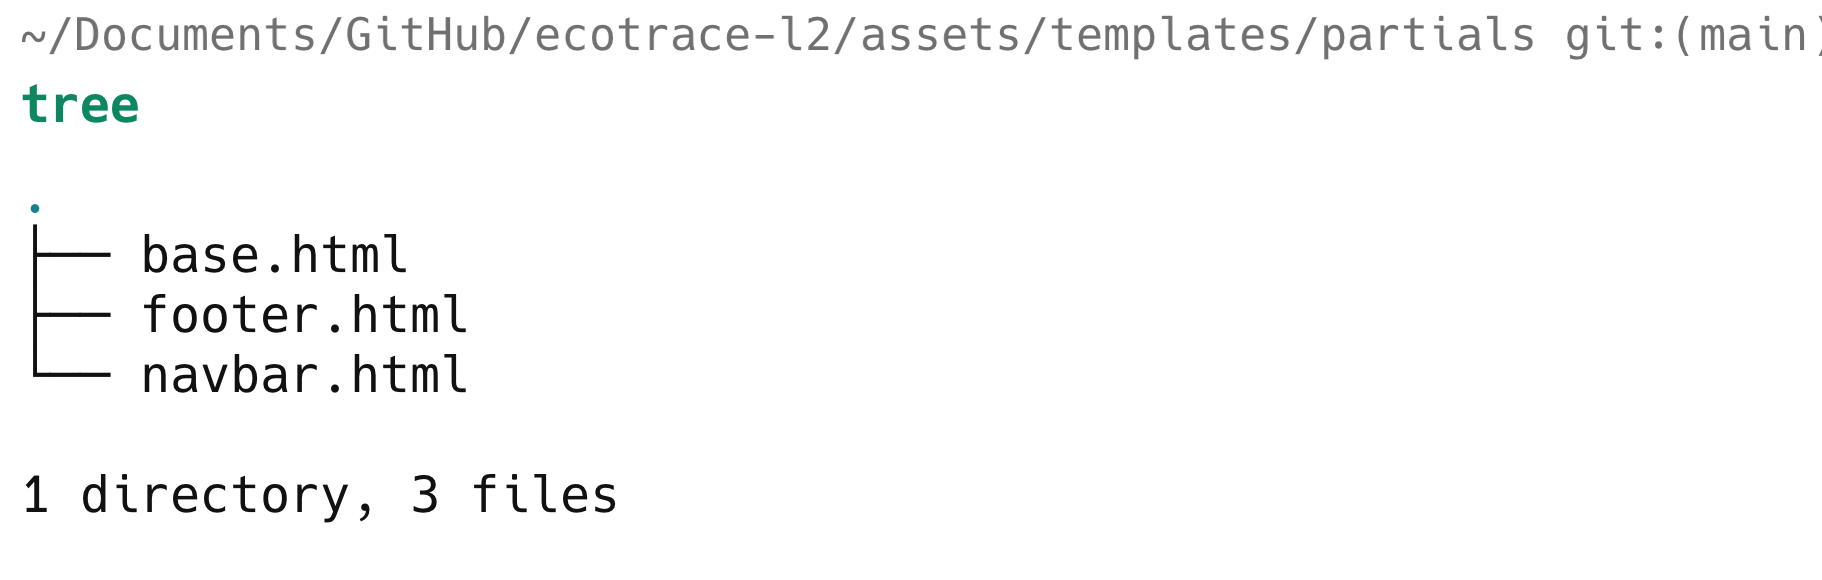
\includegraphics[width=0.7\textwidth]{captures/templates_et_static/templates/partials/img1.png}
                \end{center}

                \subsubsection{Template de base (\texttt{partials/base.html})}
                    \noindent Le template \texttt{base.html} définit la structure HTML commune à toutes les pages, incluant les liens vers les fichiers CSS et JavaScript, ainsi que les blocs pour le contenu dynamique.

                    \begin{enumerate}
                        \item \textbf{Respect des standards web et accessibilité} :
                            \begin{tcolorbox}[colback=lightgray!6, colframe=black, left=-55mm, right=5mm, top=2mm, bottom=0mm, boxrule=0.1mm]
                                \begin{verbatim}
                                    <html lang="fr" class="scroll-smooth">
                                    <meta charset="UTF-8">
                                    <meta name="viewport" content="width=device-width, initial-scale=1.0">
                                \end{verbatim}
                            \end{tcolorbox}

                        \item \textbf{SEO et métadonnées complètes} :
                            \begin{tcolorbox}[colback=lightgray!6, colframe=black, left=-65mm, right=5mm, top=2mm, bottom=0mm, boxrule=0.1mm]
                                \begin{verbatim}
                                    <title>
                                        
                                            EcoTrace - Votre compagnon pour un mode de vie durable
                                        
                                    </title>
                                    <meta name="description" content="
                                        
                                            Mesurez, comprenez et réduisez votre empreinte carbone avec EcoTrace...
                                        ">
                                    <meta name="keywords" content="empreinte carbone, écologie, développement 
                                    durable, EcoTrace, environnement, CO2">
                                \end{verbatim}
                            \end{tcolorbox}

                            \noindent Les blocs \texttt{Jinja2} permettent la personnalisation du SEO sur chaque page.

                        \item \textbf{Favicon multi-plateforme} : Un système de favicon exhaustif est mis en place pour tous les appareils et plateformes.

                        \item \textbf{Typographie et design system : Police Inter personnalisée} :
                            \begin{tcolorbox}[colback=lightgray!6, colframe=black, left=-60mm, right=5mm, top=2mm, bottom=0mm, boxrule=0.1mm]
                                \begin{verbatim}
                                    @font-face {
                                        font-family: 'Inter';
                                        src: url('{{ url_for(
                                            'static', 
                                            filename='fonts/Inter-VariableFont_opsz,wght.ttf') }}') 
                                            format('truetype-variations');
                                        font-weight: 100 900;
                                        font-style: normal;
                                        font-display: swap;
                                    }
                                \end{verbatim}
                            \end{tcolorbox}

                            \noindent Les fonctionnalités typographiques avancées sont activées pour une meilleure lisibilité :
                            \begin{tcolorbox}[colback=lightgray!6, colframe=black, left=-45mm, right=5mm, top=2mm, bottom=0mm, boxrule=0.1mm]
                                \begin{verbatim}
                                    * {
                                        font-feature-settings: 'cv11', 'ss01';
                                        font-variant-numeric: tabular-nums;
                                    }
                                \end{verbatim}
                            \end{tcolorbox}

                        \item \textbf{Palette de couleurs cohérente} : La palette est basée sur le vert émeraude, en accord avec la thématique environnementale.

                        \item \textbf{Système de messages flash} :
                            \noindent Un système de notifications visuelles sophistiqué est mis en place :
                            \begin{tcolorbox}[colback=lightgray!6, colframe=black, left=-45mm, right=5mm, top=2mm, bottom=0mm, boxrule=0.1mm]
                                \begin{verbatim}
                                    <div class="flash-message bg-white border-l-4 p-4 rounded-lg 
                                    shadow-lg max-w-sm animate-slide-up
                                    border-red-500 text-red-700
                                    border-yellow-500 text-yellow-700
                                    border-emerald-500 text-emerald-700
                                    border-blue-500 text-blue-700">
                                \end{verbatim}
                            \end{tcolorbox}

                            \noindent Chaque type de message possède une couleur, une icône, une animation et un positionnement spécifique.

                        \item \textbf{Accessibilité} :
                            \begin{itemize}
                                \item Navigation au clavier :
                                    \begin{tcolorbox}[colback=lightgray!6, colframe=black, left=-80mm, right=5mm, top=2mm, bottom=0mm, boxrule=0.1mm]
                                        \begin{verbatim}
                                            <a href="#main-content" class="sr-only focus:not-sr-only focus:absolute 
                                            focus:top-4 focus:left-4 bg-emerald-600 text-white px-4 py-2 
                                            rounded-lg z-50">
                                                Aller au contenu principal
                                            </a>
                                        \end{verbatim}
                                    \end{tcolorbox}
                                \item Focus visible :
                                    \begin{tcolorbox}[colback=lightgray!6, colframe=black, left=-45mm, right=5mm, top=2mm, bottom=0mm, boxrule=0.1mm]
                                        \begin{verbatim}
                                            .focus-ring:focus {
                                                outline: 2px solid #10b981;
                                                outline-offset: 2px;
                                            }
                                        \end{verbatim}
                                    \end{tcolorbox}
                            \end{itemize}
                    \end{enumerate}

                \subsubsection{Navigation (\texttt{partials/navbar.html})}
                    \noindent Le système de navigation s'adapte automatiquement à l'état de connexion de l'utilisateur.

                    \begin{enumerate}
                        \item \textbf{Navigation desktop} :
                            \begin{tcolorbox}[colback=lightgray!6, colframe=black, left=-45mm, right=5mm, top=2mm, bottom=0mm, boxrule=0.1mm]
                                \begin{verbatim}
                                    <div class="hidden lg:flex items-center space-x-2">
                                        
                                            <!-- Liens authentifiés -->
                                        
                                            <!-- Liens publics -->
                                        
                                    </div>
                                \end{verbatim}
                            \end{tcolorbox}

                        \item \textbf{Navigation mobile} :
                            \begin{tcolorbox}[colback=lightgray!6, colframe=black, left=-60mm, right=5mm, top=2mm, bottom=0mm, boxrule=0.1mm]
                                \begin{verbatim}
                                    <div class="lg:hidden hidden bg-white border-t border-gray-100 
                                    shadow-lg" id="mobile-menu">
                                \end{verbatim}
                            \end{tcolorbox}

                        \item \textbf{Logique d'affichage conditionnelle} :
                            \noindent La navigation change selon l'état de connexion :
                            \begin{itemize}
                                \item Utilisateur connecté : Tableau de bord, Nouvelle activité, Historique, Profil utilisateur, Déconnexion
                                \item Utilisateur non connecté : Connexion, Inscription
                            \end{itemize}

                        \item \textbf{Mise en évidence de la page active} :
                            \begin{tcolorbox}[colback=lightgray!6, colframe=black, left=-60mm, right=5mm, top=2mm, bottom=0mm, boxrule=0.1mm]
                                \begin{verbatim}
                                    <a href="{{ url_for('auth.login') }}" class="
                                    
                                        bg-gradient-to-r from-emerald-500 to-teal-600 text-white...
                                    
                                        text-gray-700 hover:text-emerald-600...
                                    ">
                                \end{verbatim}
                            \end{tcolorbox}
                    \end{enumerate}

                \subsubsection{Pied de page (\texttt{partials/footer.html})}
                    \noindent Le footer est organisé en trois colonnes principales :
                    \begin{itemize}
                        \item À propos : Logo, description de l'application
                        \item Navigation : Liens contextuels selon l'état d'authentification
                        \item Ressources : FAQ, guides, support (liens prévus pour le développement futur)
                    \end{itemize}

                    \begin{enumerate}
                        \item \textbf{Liens dynamiques} : Le footer s'adapte selon que l'utilisateur est connecté ou non.
                            \begin{tcolorbox}[colback=lightgray!6, colframe=black, left=-60mm, right=5mm, top=2mm, bottom=0mm, boxrule=0.1mm]
                                \begin{verbatim}
                                    
                                        <!-- Liens pour utilisateurs connectés -->
                                    
                                        <!-- Liens pour visiteurs -->
                                    
                                \end{verbatim}
                            \end{tcolorbox}

                        \item \textbf{Section copyright} :
                            \begin{tcolorbox}[colback=lightgray!6, colframe=black, left=-60mm, right=5mm, top=2mm, bottom=0mm, boxrule=0.1mm]
                                \begin{verbatim}
                                    <div class="border-t border-gray-300 bg-white">
                                        <div class="text-sm text-gray-600">
                                            © 2025 EcoTrace. Tous droits réservés.
                                        </div>
                                \end{verbatim}
                            \end{tcolorbox}
                    \end{enumerate}

            \subsection{Templates d'authentification (\texttt{auth/})}
                \noindent Les templates d'authentification sont situés dans le répertoire \texttt{auth/}. Ils incluent les pages de connexion, d'inscription et de tableau de bord utilisateur.

                \begin{center}
                    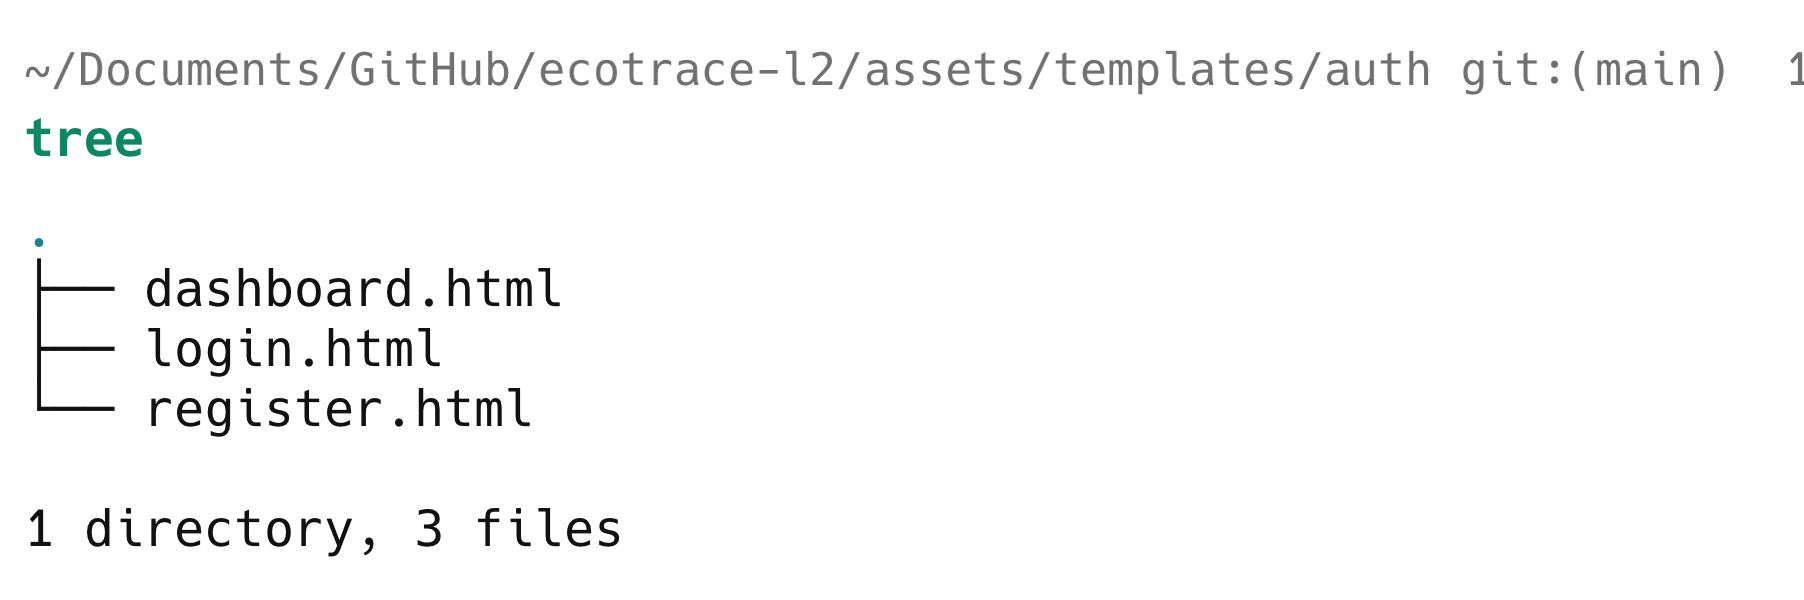
\includegraphics[width=0.7\textwidth]{captures/templates_et_static/templates/auth/auth.png}
                \end{center}

                \noindent Tous les templates partagent :

                \textbf{En-tête décoratif commun} :
                \begin{tcolorbox}[colback=lightgray!6, colframe=black, left=-45mm, right=5mm, top=2mm, bottom=0mm, boxrule=0.1mm]
                    \begin{verbatim}
                        <section class="w-full bg-gradient-to-br from-emerald-100 via-teal-50 
                        to-cyan-50 relative overflow-hidden">
                            <!-- Formes décoratives en arrière-plan -->
                            <div class="absolute inset-0 opacity-15">
                                <div class="absolute top-0 left-0 w-80 h-80 bg-gradient-to-r 
                                from-emerald-300 to-teal-400 rounded-full blur-3xl transform 
                                -translate-x-1/2 -translate-y-1/2"></div>
                                <div class="absolute bottom-0 right-0 w-64 h-64 bg-gradient-to-r 
                                from-teal-300 to-cyan-400 rounded-full blur-3xl transform 
                                translate-x-1/2 translate-y-1/2"></div>
                            </div>
                        </section>
                    \end{verbatim}
                \end{tcolorbox}

                \noindent Cette section crée un arrière-plan dynamique avec des formes floues pour donner de la profondeur visuelle.

                \subsubsection{Template d'inscription (\texttt{auth/register.html})}
                    \begin{enumerate}
                        \item \textbf{Titre et message adaptatif} :
                            \begin{tcolorbox}[colback=lightgray!6, colframe=black, left=-60mm, right=5mm, top=2mm, bottom=0mm, boxrule=0.1mm]
                                \begin{verbatim}
                                    <h1 class="text-5xl font-black bg-gradient-to-r from-emerald-700 
                                    via-teal-600 to-cyan-600 bg-clip-text text-transparent">
                                        Rejoignez EcoTrace
                                    </h1>
                                    <p class="text-lg text-gray-700 max-w-2xl leading-relaxed">
                                        Commencez votre voyage vers un mode de vie plus durable et 
                                        suivez votre empreinte carbone
                                    </p>
                                \end{verbatim}
                            \end{tcolorbox}

                        \item \textbf{Indicateurs sociaux} : Des éléments de preuve sociale rassurent les nouveaux utilisateurs.
                            \begin{tcolorbox}[colback=lightgray!6, colframe=black, left=-70mm, right=5mm, top=2mm, bottom=0mm, boxrule=0.1mm]
                                \begin{verbatim}
                                    <div class="flex items-center space-x-3 mt-2">
                                        <div class="flex -space-x-2">
                                            <div class="w-7 h-7 rounded-full bg-gradient-to-r from-emerald-400
                                            to-emerald-500 border-2 border-white"></div>
                                            <div class="w-7 h-7 rounded-full bg-gradient-to-r from-teal-400 
                                            to-teal-500 border-2 border-white"></div>
                                            <div class="w-7 h-7 rounded-full bg-gradient-to-r from-cyan-400 
                                            to-cyan-500 border-2 border-white"></div>
                                        </div>
                                        <span class="text-sm text-gray-600 font-medium">
                                            Déjà plus de 1000+ utilisateurs engagés
                                        </span>
                                    </div>
                                \end{verbatim}
                            \end{tcolorbox}

                        \item \textbf{Formulaire avec validation visuelle} :
                            \begin{tcolorbox}[colback=lightgray!6, colframe=black, left=-70mm, right=5mm, top=2mm, bottom=0mm, boxrule=0.1mm]
                                \begin{verbatim}
                                    <div class="relative">
                                        <div class="absolute inset-y-0 left-0 pl-3 flex items-center 
                                        pointer-events-none">
                                            <svg fill="none" stroke="currentColor" class="...">
                                               ...
                                            </svg>
                                        </div>
                                        {{ form.name(class="block w-full pl-10 pr-3 py-3 border ...") }}
                                    </div>
                                \end{verbatim}
                            \end{tcolorbox}

                            \noindent Chaque champ inclut une icône, des bordures arrondies, des états de focus en vert émeraude et une validation d'erreur avec icône.

                        \item \textbf{Gestion d'erreurs intégrée} :
                            \begin{tcolorbox}[colback=lightgray!6, colframe=black, left=-60mm, right=5mm, top=2mm, bottom=0mm, boxrule=0.1mm]
                                \begin{verbatim}
                                    
                                        
                                            <p class="text-red-500 text-xs mt-2 flex items-center">
                                                <svg fill="currentColor" class="w-4 ..." viewBox="0 0 20 20">
                                                    ...
                                                </svg>
                                                {{ error }}
                                            </p>
                                        
                                    
                                \end{verbatim}
                            \end{tcolorbox}
                    \end{enumerate}

                \subsubsection{Template de connexion (\texttt{auth/login.html})}
                    \noindent Le template de connexion reprend la structure de celui d'inscription, avec des ajustements pour le contexte de connexion.

                    \begin{enumerate}
                        \item \textbf{Titre et message d'accueil} :
                            \begin{tcolorbox}[colback=lightgray!6, colframe=black, left=-70mm, right=5mm, top=2mm, bottom=0mm, boxrule=0.1mm]
                                \begin{verbatim}
                                    <h1 class="text-5xl font-black bg-gradient-to-r from-emerald-700 via-teal-600
                                    to-cyan-600 bg-clip-text text-transparent">
                                        Bienvenue sur Ecotrace
                                    </h1>
                                    <p class="text-lg text-gray-700 max-w-2xl leading-relaxed">
                                        Connectez-vous à votre compte pour continuer votre parcours écologique et 
                                        consulter vos données
                                    </p>
                                \end{verbatim}
                            \end{tcolorbox}

                        \item \textbf{Formulaire simplifié} : Le formulaire de connexion est épuré, avec champs email et mot de passe, option "Se souvenir de moi" et lien vers l'inscription.
                    \end{enumerate}

                \subsubsection{Template tableau de bord (\texttt{auth/dashboard.html})}
                    \noindent Ce template intègre de nombreuses fonctionnalités avancées.

                    \begin{enumerate}
                        \item \textbf{En-tête personnalisé} :
                            \begin{tcolorbox}[colback=lightgray!6, colframe=black, left=-70mm, right=5mm, top=2mm, bottom=0mm, boxrule=0.1mm]
                                \begin{verbatim}
                                    <div class="hidden lg:flex flex-col items-end space-y-4">
                                        <div class="bg-white/70 backdrop-blur-md rounded-2xl p-8 shadow-xl 
                                        border border-white/20">
                                            <div class="w-16 h-16 bg-gradient-to-r from-emerald-400 to-teal-500 
                                            rounded-2xl flex items-center justify-center shadow-lg mx-auto mb-4">
                                                <svg class="w-8 ..." fill="none" stroke="currentColor" ...>
                                                    ...
                                                </svg>
                                            </div>
                                            <div class="text-2xl font-bold ...">
                                                {{ user.name }}
                                            </div>
                                            <div class="text-sm text-gray-600">Heureux de vous revoir</div>
                                        </div>
                                    </div>
                                \end{verbatim}
                            \end{tcolorbox}

                        \item \textbf{Système de cartes statistiques} :
                            \begin{tcolorbox}[colback=lightgray!6, colframe=black, left=-70mm, right=5mm, top=2mm, bottom=0mm, boxrule=0.1mm]
                                \begin{verbatim}
                                    <div class="grid grid-cols-1 md:grid-cols-3 gap-6">
                                        <div class="bg-white rounded-2xl shadow-md border border-gray-100 
                                        p-6 transform transition-all duration-300 hover:-translate-y-1 
                                        hover:shadow-lg">
                                            <div class="flex items-center justify-between">
                                                <div>
                                                    <p class="text-sm text-gray-600 ...">
                                                        Total mensuel
                                                    </p>
                                                    <p class="text-2xl ..." id="totalEmissions">-</p>
                                                    <p class="text-xs text-gray-500">kgCO₂e</p>
                                                </div>
                                                <div class="w-12 h-12 bg-gradient-to-r from-red-500 to-rose-600 
                                                rounded-xl flex items-center justify-center shadow-lg">
                                                    <!-- Icône SVG -->
                                                </div>
                                            </div>
                                        </div>
                                    </div>
                                \end{verbatim}
                            \end{tcolorbox}

                            \noindent Les cartes sont animées au survol, avec des icônes colorées et des données mises à jour dynamiquement.

                        \item \textbf{Intégration des graphiques} :
                            \begin{tcolorbox}[colback=lightgray!6, colframe=black, left=-70mm, right=5mm, top=2mm, bottom=0mm, boxrule=0.1mm]
                                \begin{verbatim}
                                    <div class="grid grid-cols-1 lg:grid-cols-2 gap-6">
                                        <div class="bg-white rounded-2xl shadow-md border border-gray-100 p-6">
                                            <h3 class="text-lg font-bold text-gray-900 mb-4">
                                                Répartition par catégorie
                                            </h3>
                                            <div class="relative h-64">
                                                <canvas id="categoryChart"></canvas>
                                            </div>
                                        </div>
                                    </div>
                                \end{verbatim}
                            \end{tcolorbox}

                        \item \textbf{Système de recommandations} :
                            \begin{tcolorbox}[colback=lightgray!6, colframe=black, left=-70mm, right=5mm, top=2mm, bottom=0mm, boxrule=0.1mm]
                                \begin{verbatim}
                                    <div class="bg-white rounded-2xl shadow-md border border-gray-100 
                                    overflow-hidden">
                                        <div class="p-6 border-b border-gray-100">
                                            <div class="flex items-center justify-between">
                                                <!-- Titre et description -->
                                                <div class="flex gap-2">
                                                    <button class="px-3 py-2 bg-emerald-100 text-emerald-700 
                                                    rounded-lg text-sm font-medium hover:bg-emerald-200 
                                                    transition-colors duration-200 filter-btn active" 
                                                    data-filter="all">
                                                        Toutes
                                                    </button>
                                                    <!-- Autres filtres -->
                                                </div>
                                            </div>
                                        </div>
                                    </div>
                                \end{verbatim}
                            \end{tcolorbox}

                            \noindent Le système de recommandations propose des filtres interactifs et des badges colorés.

                        \item \textbf{Actions rapides} :
                            \begin{tcolorbox}[colback=lightgray!6, colframe=black, left=-70mm, right=5mm, top=2mm, bottom=0mm, boxrule=0.1mm]
                                \begin{verbatim}
                                    <div class="flex flex-col sm:flex-row gap-3">
                                        <a href="{{ url_for('carbon.add_activity') }}" 
                                        class="bg-gradient-to-r from-emerald-500 to-teal-600 text-white 
                                        px-6 py-3 rounded-xl font-bold hover:from-emerald-600 
                                        hover:to-teal-700 transition-all duration-300 shadow-lg 
                                        hover:shadow-xl transform hover:-translate-y-1 flex 
                                        items-center space-x-2">
                                            <svg class="w-5 h-5" fill="none" stroke="currentColor" ...>
                                                ...
                                            </svg>
                                            <span>Nouvelle activité</span>
                                        </a>
                                    </div>
                                \end{verbatim}
                            \end{tcolorbox}

                        \item \textbf{Profil utilisateur moderne} :
                            \begin{tcolorbox}[colback=lightgray!6, colframe=black, left=-70mm, right=5mm, top=2mm, bottom=0mm, boxrule=0.1mm]
                                \begin{verbatim}
                                    <div class="divide-y divide-gray-100">
                                        <div class="p-6 hover:bg-gray-50 transition-colors duration-200">
                                            <div class="flex items-center justify-between">
                                                <div class="flex items-center space-x-3">
                                                    <div class="w-10 h-10 bg-gradient-to-r from-blue-500 
                                                    to-indigo-600 rounded-lg flex items-center justify-center">
                                                        <svg class="w-5 h-5 text-white" fill="none" ...>
                                                            ...
                                                        </svg>
                                                    </div>
                                                    <div>
                                                        <p class="text-sm font-medium text-gray-900">Nom</p>
                                                        <p class="text-sm text-gray-500">Votre nom complet</p>
                                                    </div>
                                                </div>
                                                <span class="text-sm font-semibold ...">
                                                    {{ user.name }}
                                                </span>
                                            </div>
                                        </div>
                                    </div>
                                \end{verbatim}
                            \end{tcolorbox}

                        \item \textbf{Intégration JavaScript} :
                            \begin{tcolorbox}[colback=lightgray!6, colframe=black, left=-70mm, right=5mm, top=2mm, bottom=0mm, boxrule=0.1mm]
                                \begin{verbatim}
                                    <script>
                                        const categoriesData = {{ categories_data| safe }};
                                        const weeklyData = {{ weekly_trend| safe }};
                                        const monthlySummary = {{ monthly_summary| safe }};
                                    </script>
                                    <script src="{{ url_for('static', filename='js/dashboard.js') }}"></script>
                                \end{verbatim}
                            \end{tcolorbox}

                            \noindent Les données sont préparées côté serveur au format JSON pour Chart.js côté client.
                    \end{enumerate}

            \subsection{Templates du module carbone (\texttt{carbon/})}
                \noindent Les templates du module \texttt{carbon/} sont conçus pour encourager l'action et l'engagement écologique. Chaque template conserve la cohérence visuelle tout en adaptant le message à sa fonction.

                \begin{center}
                    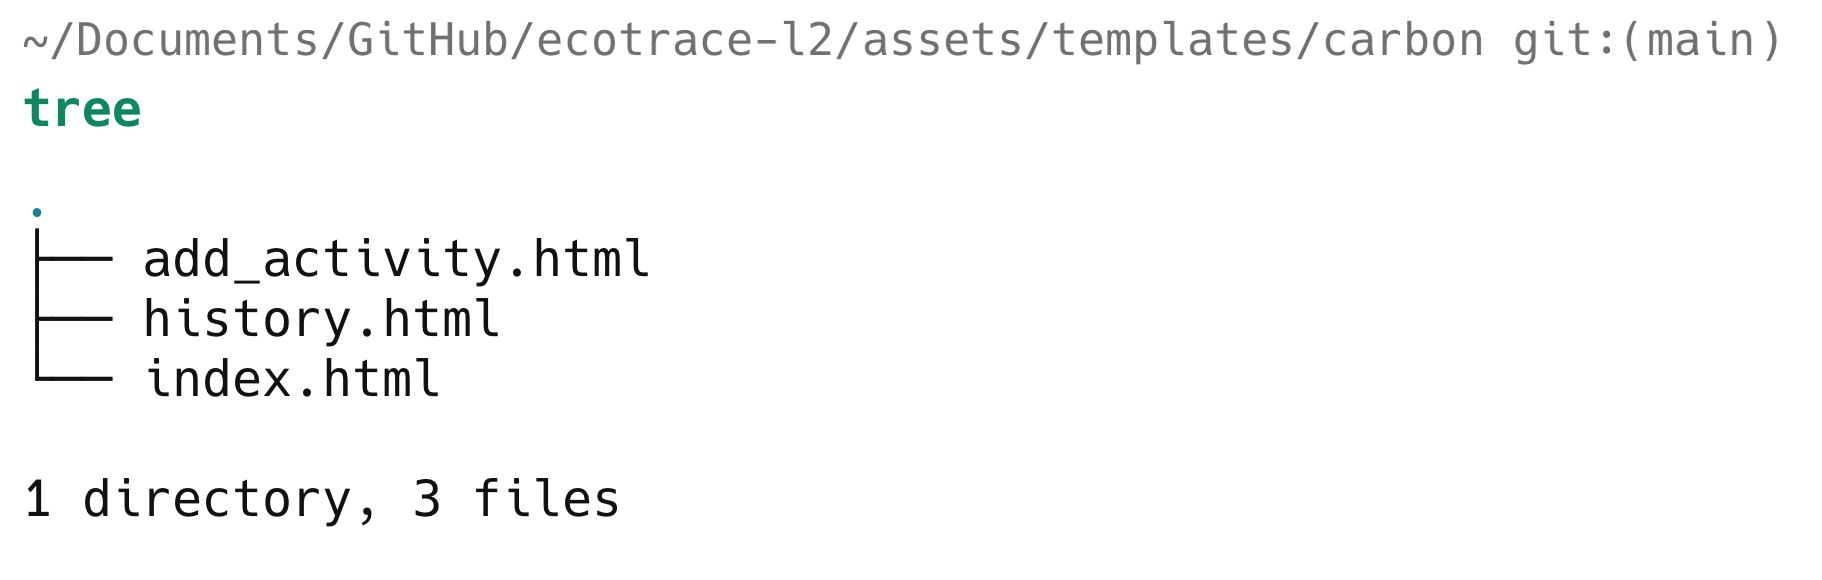
\includegraphics[width=0.7\textwidth]{captures/templates_et_static/templates/carbon/img1.png}
                \end{center}

                \subsubsection{Template d'accueil (\texttt{carbon/index.html})}
                    \begin{enumerate}
                        \item \textbf{Page d'accueil marketing complète} :
                            \begin{tcolorbox}[colback=lightgray!6, colframe=black, left=-70mm, right=5mm, top=2mm, bottom=0mm, boxrule=0.1mm]
                                \begin{verbatim}
                                    <h1 class="text-5xl font-black bg-gradient-to-r from-emerald-700 
                                    via-teal-600 to-cyan-600 bg-clip-text text-transparent">
                                        Bienvenue sur EcoTrace
                                    </h1>
                                    <p class="text-xl text-gray-700 max-w-2xl leading-relaxed">
                                        Transformez votre mode de vie avec l'application qui vous aide à 
                                        mesurer, comprendre et réduire votre empreinte carbone au quotidien.
                                    </p>
                                \end{verbatim}
                            \end{tcolorbox}

                        \item \textbf{Intégration de données dynamiques} :
                            \begin{tcolorbox}[colback=lightgray!6, colframe=black, left=-70mm, right=5mm, top=2mm, bottom=0mm, boxrule=0.1mm]
                                \begin{verbatim}
                                    <span class="text-sm text-gray-600 font-medium">
                                        Rejoignez plus de {{ total_users }} éco-citoyens engagés
                                    </span>
                                \end{verbatim}
                            \end{tcolorbox}

                            \noindent Les variables de contexte affichent des statistiques en temps réel pour renforcer la crédibilité et l'engagement communautaire.

                        \item \textbf{Boutons d'appel à l'action} :
                            \begin{tcolorbox}[colback=lightgray!6, colframe=black, left=-70mm, right=5mm, top=2mm, bottom=0mm, boxrule=0.1mm]
                                \begin{verbatim}
                                    <div class="flex flex-col sm:flex-row gap-4 mt-8">
                                        <a href="{{ url_for('auth.register') }}" 
                                        class="bg-gradient-to-r from-emerald-500 to-teal-600 text-white
                                         px-8 py-4 rounded-xl font-bold hover:from-emerald-600 
                                         hover:to-teal-700 transition-all duration-300 shadow-lg 
                                         hover:shadow-xl transform hover:-translate-y-1 flex items-center 
                                         justify-center space-x-2">
                                            <svg fill="none" stroke="currentColor" class="w-5 h-5" ...>
                                                ...
                                            </svg>
                                            <span>Commencer maintenant</span>
                                        </a>
                                    </div>
                                \end{verbatim}
                            \end{tcolorbox}
                    \end{enumerate}

                \subsubsection{Template d'ajout d'activité (\texttt{carbon/add\_activity.html})}
                    \noindent Ce template intègre de nombreuses innovations UX.

                    \begin{enumerate}
                        \item \textbf{Sélecteur de catégories interactif} :
                            \begin{tcolorbox}[colback=lightgray!6, colframe=black, left=-70mm, right=5mm, top=2mm, bottom=0mm, boxrule=0.1mm]
                                \begin{verbatim}
                                    <div class="grid grid-cols-1 sm:grid-cols-2 lg:grid-cols-4 gap-4">
                                        <div class="category-option cursor-pointer group" 
                                        data-category="transport">
                                            <input type="radio" name="category" id="transport" value="transport"
                                             class="hidden"/>
                                            <label for="transport" class="block border-2 border-gray-200 
                                            rounded-xl p-6 text-center hover:border-emerald-400 
                                            hover:bg-emerald-50 transition-all duration-300 
                                            group-hover:shadow-lg group-hover:scale-105">
                                                <div class="w-12 h-12 bg-blue-100 rounded-xl flex 
                                                items-center justify-center group-hover:bg-blue-500 
                                                transition-colors duration-300">
                                                    <svg fill="none" stroke="currentColor" ...>
                                                        ...
                                                    </svg>
                                                </div>
                                            </label>
                                        </div>
                                    </div>
                                \end{verbatim}
                            \end{tcolorbox}

                            \noindent Chaque catégorie possède une couleur thématique, des animations au survol et des icônes SVG personnalisées.

                        \item \textbf{Dropdowns personnalisés avancés} :
                            \begin{tcolorbox}[colback=lightgray!6, colframe=black, left=-70mm, right=5mm, top=2mm, bottom=0mm, boxrule=0.1mm]
                                \begin{verbatim}
                                    <div class="custom-dropdown relative" data-target="transport">
                                        <div class="selected-option flex justify-between items-center 
                                        w-full px-4 py-3 border-2 border-gray-200 placeholder-gray-500 
                                        text-gray-900 rounded-xl focus:outline-none focus:ring-2 
                                        focus:ring-emerald-500 focus:border-emerald-500 bg-white 
                                        cursor-pointer hover:border-emerald-300 transition-all 
                                        duration-300 shadow-sm">
                                            <span class="selected-text text-gray-500">
                                                Sélectionnez un type de transport
                                            </span>
                                            <svg fill="none" stroke="currentColor" ...>
                                                ...
                                            </svg>
                                        </div>
                                        <div class="options-container hidden absolute z-10 left-0 
                                        right-0 mt-2 max-h-60 overflow-y-auto bg-white border 
                                        border-gray-200 rounded-xl shadow-xl">
                                            
                                            <div class="option px-4 py-3 hover:bg-emerald-50 
                                            cursor-pointer border-b border-gray-100 text-sm 
                                            transition-colors duration-200" 
                                            data-value="{{ factor.id }}" data-unit="{{ factor.unit }}">
                                                {{ factor.activity_name }}
                                            </div>
                                            
                                        </div>
                                    </div>
                                \end{verbatim}
                            \end{tcolorbox}

                            \noindent Les dropdowns sont entièrement personnalisés pour une meilleure expérience utilisateur.

                        \item \textbf{Calendrier personnalisé} :
                            \begin{tcolorbox}[colback=lightgray!6, colframe=black, left=-70mm, right=5mm, top=2mm, bottom=0mm, boxrule=0.1mm]
                                \begin{verbatim}
                                    <div class="custom-date-dropdown relative overflow-visible">
                                        <div class="calendar-container hidden absolute z-50 left-0 
                                        right-0 mt-2 bg-white border border-gray-200 rounded-xl 
                                        shadow-xl p-4">
                                            <div class="calendar-header flex justify-between 
                                            items-center mb-4">
                                                <button type="button" class="prev-month p-2 
                                                hover:bg-emerald-50 rounded-full transition-colors
                                                duration-200">
                                                    <svg fill="none" stroke="currentColor" ...>
                                                        ...
                                                    </svg>
                                                </button>
                                                <div class="month-year font-semibold text-gray-900"></div>
                                                <button type="button" class="next-month p-2 hover:bg-emerald-50 
                                                rounded-full transition-colors duration-200">
                                                    <svg fill="none" stroke="currentColor" ...>
                                                        ...
                                                    </svg>
                                                </button>
                                            </div>
                                            <div class="weekdays grid grid-cols-7 gap-1 mb-2 text-center 
                                            text-xs text-gray-500 font-medium">
                                                <div>Lu</div>
                                                <div>Ma</div>
                                                <div>Me</div>
                                                <div>Je</div>
                                                <div>Ve</div>
                                                <div>Sa</div>
                                                <div>Di</div>
                                            </div>
                                            <div class="days-grid grid grid-cols-7 gap-1"></div>
                                        </div>
                                    </div>
                                \end{verbatim}
                            \end{tcolorbox}

                            \noindent Le calendrier permet la navigation entre les mois et une sélection rapide de la date.
                    \end{enumerate}

                \subsubsection{Template d'historique (\texttt{carbon/history.html})}
                    \noindent Ce template affiche l'historique des activités de l'utilisateur avec une interface lisible et intuitive.

                    \begin{enumerate}
                        \item \textbf{Affichage conditionnel intelligent} :
                            \begin{tcolorbox}[colback=lightgray!5, colframe=gray!80, left=-70mm, right=5mm, top=2mm, bottom=0mm, boxrule=0.1mm]
                                \begin{verbatim}
                                    
                                        <!-- Contenu avec données -->
                                    
                                        <!-- État vide avec encouragement -->
                                        <div class="bg-white rounded-2xl shadow-md border 
                                        border-gray-100 overflow-hidden">
                                            <div class="text-center py-16 px-8">
                                                <div class="w-24 h-24 bg-gradient-to-r 
                                                from-emerald-400 to-teal-500 rounded-full flex 
                                                items-center justify-center shadow-lg mx-auto mb-8">
                                                    <svg fill="none" stroke="currentColor" ...>
                                                        ...
                                                    </svg>
                                                </div>
                                                <h2 class="text-2xl font-bold text-gray-900 mb-4">
                                                    Votre historique est encore vide
                                                </h2>
                                            </div>
                                        </div>
                                    
                                \end{verbatim}
                            \end{tcolorbox}

                        \item \textbf{Statistiques calculées dynamiquement} :
                            \begin{tcolorbox}[colback=lightgray!5, colframe=gray!80, left=-70mm, right=5mm, top=2mm, bottom=0mm, boxrule=0.1mm]
                                \begin{verbatim}
                                    <div class="grid grid-cols-1 md:grid-cols-2 lg:grid-cols-4 gap-6">
                                        <div class="bg-white rounded-2xl shadow-md border border-gray-100 
                                        p-6 transform transition-all duration-300 hover:-translate-y-1 
                                        hover:shadow-lg">
                                            <div class="flex items-center justify-between">
                                                <div>
                                                    <p class="text-sm text-gray-600 font-medium">
                                                        Total activités
                                                    </p>
                                                    <p class="text-2xl font-bold text-gray-900">
                                                        {{ activities_json|length }}
                                                    </p>
                                                    <p class="text-xs text-gray-500">enregistrées</p>
                                                </div>
                                                <div class="w-12 h-12 bg-gradient-to-r from-emerald-500 
                                                to-teal-600 rounded-xl flex items-center justify-center 
                                                shadow-lg">
                                                    <svg fill="none" stroke="currentColor" ...">
                                                        ...
                                                    </svg>
                                                </div>
                                            </div>
                                        </div>
                                    </div>
                                \end{verbatim}
                            \end{tcolorbox}

                        \item \textbf{Interface responsive avancée} :
                            \begin{tcolorbox}[colback=lightgray!5, colframe=gray!80, left=-70mm, right=5mm, top=2mm, bottom=0mm, boxrule=0.1mm]
                                \begin{verbatim}
                                    <!-- Version desktop : tableau -->
                                    <div class="hidden lg:block overflow-x-auto">
                                        <table class="min-w-full divide-y divide-gray-200" id="activitiesTable">
                                            <thead class="bg-gray-50">
                                                <tr>
                                                    <th class="px-6 py-3 text-left text-xs font-medium 
                                                    text-gray-500 uppercase tracking-wider">Date</th>
                                                    <!-- Autres colonnes -->
                                                </tr>
                                            </thead>
                                        </table>
                                    </div>

                                    <!-- Version mobile : cartes -->
                                    <div class="lg:hidden p-6 space-y-4" id="activitiesCards">
                                        
                                        <div class="bg-gray-50 rounded-xl p-4 activity-card">
                                            <!-- Contenu de la carte -->
                                        </div>
                                        
                                    </div>
                                \end{verbatim}
                            \end{tcolorbox}

                            \noindent Deux interfaces sont proposées : tableau pour desktop, cartes pour mobile.

                        \item \textbf{Badges de catégories colorés} :
                            \begin{tcolorbox}[colback=lightgray!5, colframe=gray!80, left=-70mm, right=5mm, top=2mm, bottom=0mm, boxrule=0.1mm]
                                \begin{verbatim}
                                    
                                    <span class="inline-flex items-center px-2.5 py-0.5 rounded-full 
                                    text-xs font-medium bg-blue-100 text-blue-800">
                                        <svg fill="none" stroke="currentColor" ...">
                                            ...
                                        </svg>
                                        Transport
                                    </span>
                                    
                                    <span class="inline-flex items-center px-2.5 py-0.5 rounded-full 
                                    text-xs font-medium bg-orange-100 text-orange-800">
                                        <svg fill="none" stroke="currentColor" ...">
                                            ...
                                        </svg>
                                        Alimentation
                                    </span>
                                    
                                \end{verbatim}
                            \end{tcolorbox}
                    \end{enumerate}

            \subsection{Templates d'erreur (\texttt{errors/})}
                \noindent Les pages d'erreur sont conçues pour transformer une expérience négative en opportunité d'engagement, en restant cohérentes avec l'identité écologique d'EcoTrace.

                \begin{center}
                    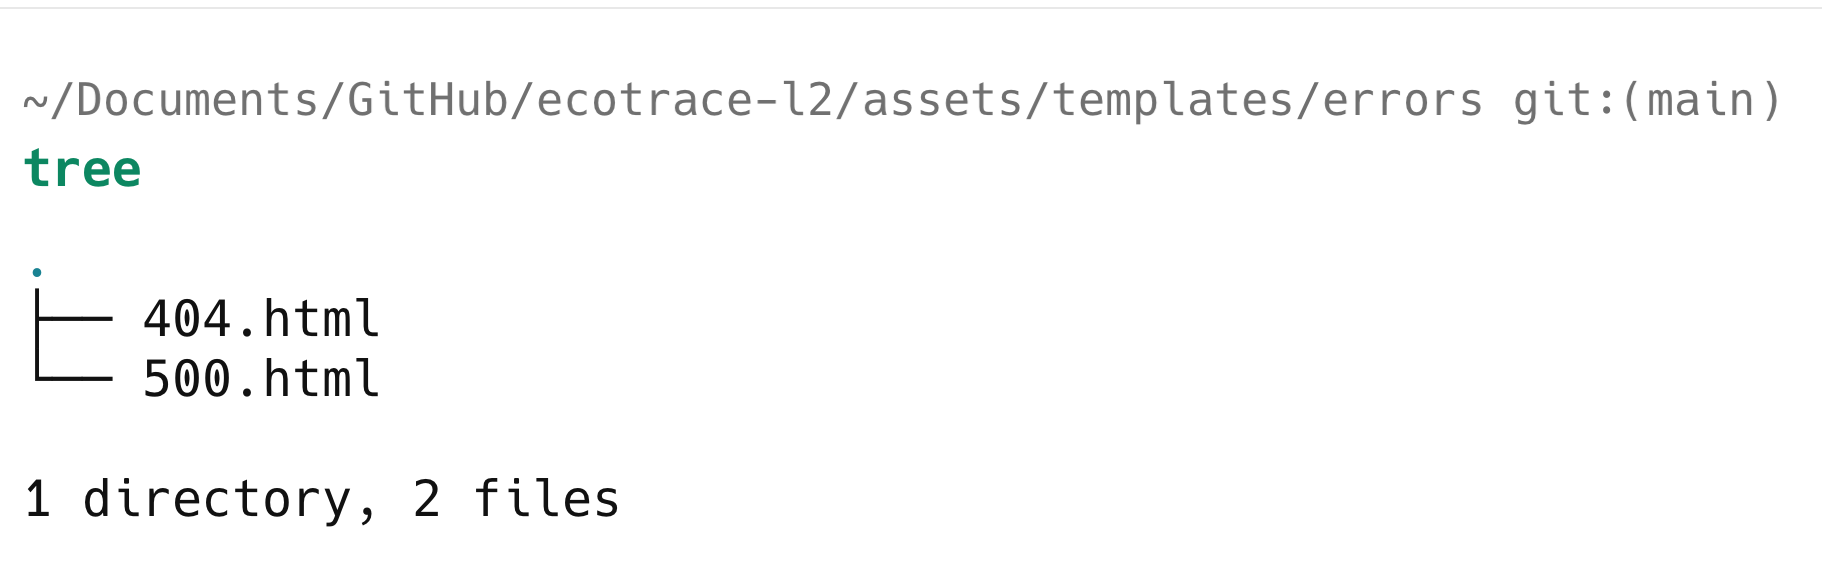
\includegraphics[width=0.7\textwidth]{captures/templates_et_static/templates/errors/img1.png}
                \end{center}

                \subsubsection{Template 404 (\texttt{errors/404.html})}
                    \begin{enumerate}
                        \item \textbf{Message humoristique et thématique} :
                            \begin{tcolorbox}[colback=lightgray!5, colframe=gray!80, left=-70mm, right=5mm, top=2mm, bottom=0mm, boxrule=0.1mm]
                                \begin{verbatim}
                                    <h1 class="text-5xl font-black bg-gradient-to-r from-emerald-700 
                                    via-teal-600 to-cyan-600 bg-clip-text text-transparent">
                                        Page introuvable
                                    </h1>
                                    <p class="text-xl text-gray-700 max-w-2xl leading-relaxed">
                                        Oups ! Il semblerait que cette page ait pris un chemin plus 
                                        écologique et ait disparu de nos serveurs.
                                    </p>
                                \end{verbatim}
                            \end{tcolorbox}

                        \item \textbf{Indicateurs visuels créatifs} :
                            \begin{tcolorbox}[colback=lightgray!5, colframe=gray!80, left=-70mm, right=5mm, top=2mm, bottom=0mm, boxrule=0.1mm]
                                \begin{verbatim}
                                    <div class="flex -space-x-2">
                                        <div class="w-8 h-8 rounded-full bg-gradient-to-r from-red-400 
                                        to-red-500 border-2 border-white flex items-center justify-center">
                                            <span class="text-xs text-white font-bold">!</span>
                                        </div>
                                        <div class="w-8 h-8 rounded-full bg-gradient-to-r from-yellow-400 
                                        to-yellow-500 border-2 border-white flex items-center justify-center">
                                            <span class="text-xs text-white font-bold">?</span>
                                        </div>
                                        <div class="w-8 h-8 rounded-full bg-gradient-to-r from-emerald-400 
                                        to-emerald-500 border-2 border-white flex items-center justify-center">
                                            <span class="text-xs text-white font-bold">✓</span>
                                        </div>
                                    </div>
                                \end{verbatim}
                            \end{tcolorbox}

                        \item \textbf{Section principale engageante} :
                            \begin{tcolorbox}[colback=lightgray!5, colframe=gray!80, left=-70mm, right=5mm, top=2mm, bottom=0mm, boxrule=0.1mm]
                                \begin{verbatim}
                                    <h2 class="text-3xl font-bold text-gray-900 mb-6">
                                        Ne perdons pas notre chemin vers la durabilité !
                                    </h2>
                                    <p class="text-lg text-gray-600 mb-8 leading-relaxed max-w-2xl mx-auto">
                                        Cette page semble avoir migré vers un serveur plus écologique. 
                                        Pendant que nous la retrouvons, explorons d'autres façons de 
                                        réduire votre empreinte carbone.
                                    </p>
                                \end{verbatim}
                            \end{tcolorbox}

                        \item \textbf{Navigation contextuelle intelligente} :
                            \begin{tcolorbox}[colback=lightgray!5, colframe=gray!80, left=-70mm, right=5mm, top=2mm, bottom=0mm, boxrule=0.1mm]
                                \begin{verbatim}
                                    
                                        <a href="{{ url_for('auth.dashboard') }}" 
                                        class="bg-white border-2 border-emerald-300 text-emerald-700 
                                        px-8 py-4 rounded-xl font-bold hover:bg-emerald-50 
                                        hover:border-emerald-400 transition-all duration-300 shadow-md 
                                        hover:shadow-lg flex items-center justify-center space-x-2">
                                            <span>Mon tableau de bord</span>
                                        </a>
                                    
                                        <a href="{{ url_for('auth.register') }}" class="bg-white 
                                        border-2 border-emerald-300 text-emerald-700 px-8 py-4 
                                        rounded-xl font-bold hover:bg-emerald-50 
                                        hover:border-emerald-400 transition-all duration-300 
                                        shadow-md hover:shadow-lg flex items-center justify-center 
                                        space-x-2">
                                            <span>Commencer avec EcoTrace</span>
                                        </a>
                                    
                                \end{verbatim}
                            \end{tcolorbox}

                        \item \textbf{Pages populaires adaptatives} :
                            \begin{tcolorbox}[colback=lightgray!5, colframe=gray!80, left=-70mm, right=5mm, top=2mm, bottom=0mm, boxrule=0.1mm]
                                \begin{verbatim}
                                    <div class="grid grid-cols-1 md:grid-cols-3 gap-8 max-w-5xl mx-auto">
                                        <a href="{{ url_for('carbon.index') }}" class="group bg-white 
                                        rounded-2xl shadow-md border border-gray-100 p-8 hover:shadow-lg
                                        hover:-translate-y-1 transition-all duration-300">
                                            <div class="w-16 h-16 bg-gradient-to-r from-emerald-500 
                                            to-teal-600 rounded-2xl flex items-center justify-center 
                                            shadow-lg mb-6 group-hover:scale-105 transition-transform 
                                            duration-300">
                                                <svg fill="none" stroke="currentColor" ...>
                                                    ...
                                                </svg>
                                            </div>
                                            <h4 class="text-xl font-bold text-gray-900 mb-3">Accueil</h4>
                                            <p class="text-gray-600 leading-relaxed">
                                                Découvrez EcoTrace et commencez votre parcours vers un 
                                                mode de vie durable.
                                            </p>
                                        </a>
                                    </div>
                                \end{verbatim}
                            \end{tcolorbox}
                    \end{enumerate}

                \subsubsection{Template 500 (\texttt{errors/500.html})}
                    \begin{enumerate}
                        \item \textbf{Thématique de maintenance écologique} :
                            \begin{tcolorbox}[colback=lightgray!5, colframe=gray!80, left=-70mm, right=5mm, top=2mm, bottom=0mm, boxrule=0.1mm]
                                \begin{verbatim}
                                    <h1 class="text-5xl font-black bg-gradient-to-r from-emerald-700 
                                    via-teal-600 to-cyan-600 bg-clip-text text-transparent">
                                        Serveur en maintenance
                                    </h1>
                                    <p class="text-xl text-gray-700 max-w-2xl leading-relaxed">
                                        Notre serveur prend une pause écologique pour se régénérer. 
                                        Nous travaillons activement pour rétablir le service.
                                    </p>
                                \end{verbatim}
                            \end{tcolorbox}

                        \item \textbf{Indicateurs progressifs} :
                            \begin{tcolorbox}[colback=lightgray!5, colframe=gray!80, left=-70mm, right=5mm, top=2mm, bottom=0mm, boxrule=0.1mm]
                                \begin{verbatim}
                                    <div class="flex -space-x-2">
                                        <div class="w-8 h-8 rounded-full bg-gradient-to-r from-red-400 
                                        to-red-500 border-2 border-white flex items-center justify-center">
                                            <svg fill="none" stroke="currentColor" ...>
                                                ...
                                            </svg>
                                        </div>
                                        <div class="w-8 h-8 rounded-full bg-gradient-to-r from-orange-400 
                                        to-orange-500 border-2 border-white flex items-center justify-center">
                                            <svg fill="none" stroke="currentColor" ...>
                                                ...
                                            </svg>
                                        </div>
                                        <div class="w-8 h-8 rounded-full bg-gradient-to-r from-emerald-400 
                                        to-emerald-500 border-2 border-white flex items-center justify-center">
                                            <svg fill="none" stroke="currentColor" ...>
                                                ...
                                            </svg>
                                        </div>
                                    </div>
                                \end{verbatim}
                            \end{tcolorbox}

                        \item \textbf{Guide d'action utilisateur} :
                            \begin{tcolorbox}[colback=lightgray!5, colframe=gray!80, left=-70mm, right=5mm, top=2mm, bottom=0mm, boxrule=0.1mm]
                                \begin{verbatim}
                                    <div class="grid grid-cols-1 md:grid-cols-3 gap-6">
                                        <div class="text-center p-6 bg-gradient-to-r from-blue-50 to-blue-100 
                                        rounded-xl border border-blue-200">
                                            <div class="w-12 h-12 bg-blue-500 rounded-xl flex items-center 
                                            justify-center mx-auto mb-4">
                                                <svg fill="none" stroke="currentColor"...>
                                                    ...
                                                </svg>
                                            </div>
                                            <h4 class="font-semibold text-gray-900 mb-2">
                                                Rechargez la page
                                            </h4>
                                            <p class="text-sm text-gray-600">
                                                Actualisez votre navigateur dans quelques minutes
                                            </p>
                                        </div>
                                    </div>
                                \end{verbatim}
                            \end{tcolorbox}

                        \item \textbf{Bouton de rechargement interactif} :
                            \begin{tcolorbox}[colback=lightgray!5, colframe=gray!80, left=-70mm, right=5mm, top=2mm, bottom=0mm, boxrule=0.1mm]
                                \begin{verbatim}
                                    <button onclick="window.location.reload()" 
                                    class="bg-gradient-to-r from-emerald-500 to-teal-600 text-white 
                                    px-8 py-4 rounded-xl font-bold hover:from-emerald-600 
                                    hover:to-teal-700 transition-all duration-300 shadow-lg 
                                    hover:shadow-xl transform hover:-translate-y-1 flex items-center 
                                    justify-center space-x-2">
                                        <svg fill="none" stroke="currentColor" ...>
                                            ...
                                        </svg>
                                        <span>Réessayer maintenant</span>
                                    </button>
                                \end{verbatim}
                            \end{tcolorbox}

                        \item \textbf{Section engagement environnemental} :
                            \begin{tcolorbox}[colback=lightgray!5, colframe=gray!80, left=-70mm, right=5mm, top=2mm, bottom=0mm, boxrule=0.1mm]
                                \begin{verbatim}
                                    <div class="bg-gradient-to-r from-gray-50 to-gray-100 rounded-2xl 
                                    p-8 border border-gray-200">
                                        <h3 class="text-xl font-bold text-gray-900 mb-6 text-center">
                                            Notre engagement environnemental
                                        </h3>
                                        <div class="grid grid-cols-1 md:grid-cols-2 gap-6">
                                            <div class="flex items-start space-x-3">
                                                <div class="w-8 h-8 bg-emerald-500 rounded-lg flex 
                                                items-center justify-center flex-shrink-0">
                                                    <svg fill="none" stroke="currentColor"...>...</svg>
                                                </div>
                                                <div>
                                                    <h4 class="font-semibold text-gray-900 mb-1">
                                                        Serveurs verts
                                                    </h4>
                                                    <p class="text-sm text-gray-600">
                                                        Alimentés par des énergies renouvelables
                                                    </p>
                                                </div>
                                            </div>
                                        </div>
                                    </div>
                                \end{verbatim}
                            \end{tcolorbox}
                    \end{enumerate}

            \bigskip
            \textbf{LES STATIQUES}\\\\
            \noindent Les fichiers statiques (CSS, JavaScript, fonts, images, favicon) sont gérés par Flask et organisés dans le répertoire \texttt{static/}. Ils sont utilisés pour styliser les templates et ajouter des fonctionnalités interactives.

            \subsection{Les fichiers JavaScript (\texttt{static/js})}
                \noindent J'ai organisé le code JavaScript en modules spécialisés selon leurs responsabilités :

                \begin{center}
                    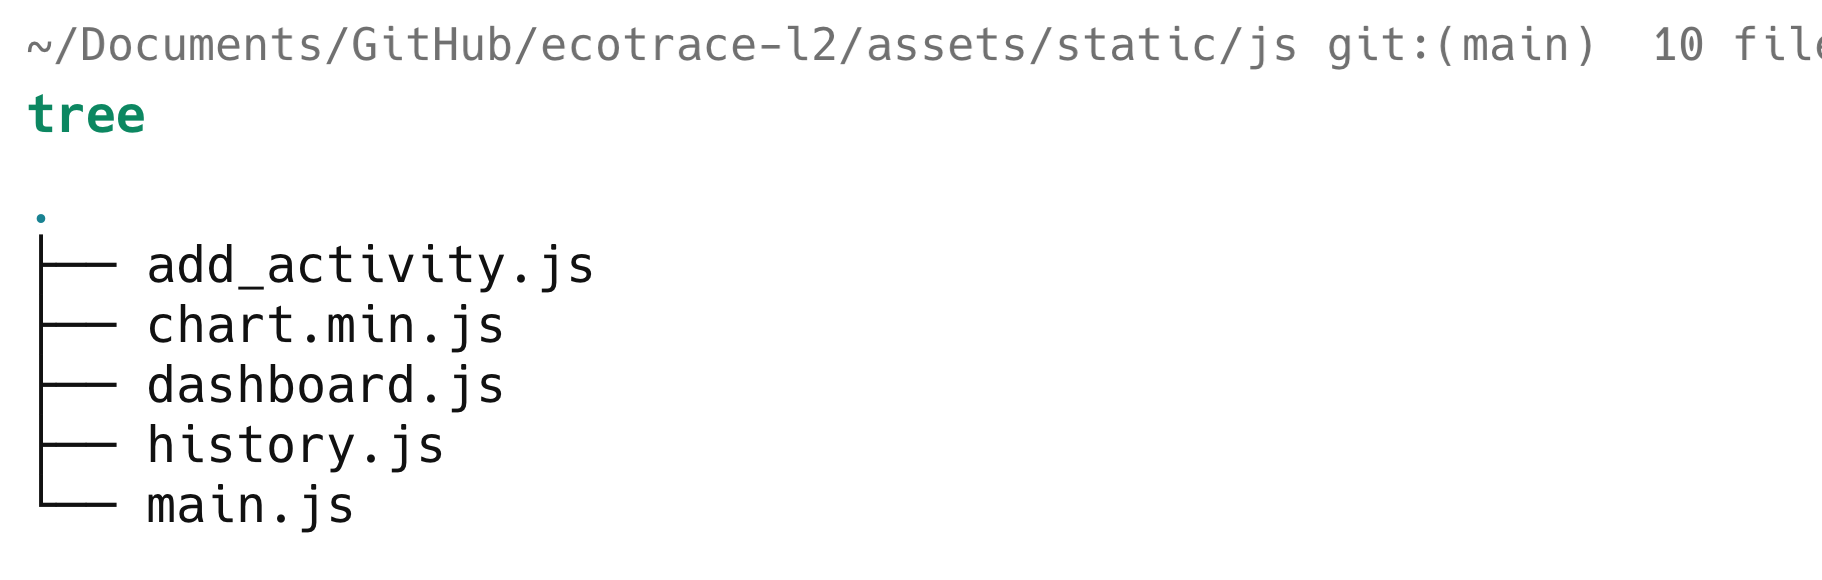
\includegraphics[width=0.7\textwidth]{captures/templates_et_static/static/js/img1.png}
                \end{center}

                \begin{itemize}
                    \item \texttt{main.js} : Fonctionnalités globales et utilitaires partagés
                    \item \texttt{add\_activity.js} : Logique spécifique au formulaire d'ajout d'activité
                    \item \texttt{dashboard.js} : Gestion du tableau de bord et des graphiques
                    \item \texttt{history.js} : Interface d'historique avec graphiques et tri
                    \item \texttt{chart.min.js} : Bibliothèque Chart.js pour les visualisations
                \end{itemize}

                \noindent Cette approche modulaire facilite la maintenance et optimise les performances en chargeant uniquement les scripts nécessaires à chaque page.

                \subsubsection{Fichier principal (\texttt{main.js})}
                    \begin{itemize}
                        \item \textbf{Architecture globale et utilitaires}:
                            \begin{tcolorbox}[colback=lightgray!5, colframe=gray!80, left=-70mm, right=5mm, top=2mm, bottom=0mm, boxrule=0.1mm]
                                \begin{verbatim}
                                    document.addEventListener('DOMContentLoaded', function() {
                                        initMobileNavigation();
                                        initFlashMessages();
                                        initSmoothScrolling();
                                        initLazyLoading();
                                    });
                                \end{verbatim}
                            \end{tcolorbox}

                        \item \textbf{Gestion du loader de page}:
                            \begin{tcolorbox}[colback=lightgray!5, colframe=gray!80, left=-70mm, right=5mm, top=2mm, bottom=0mm, boxrule=0.1mm]
                                \begin{verbatim}
                                    window.addEventListener('load', function() {
                                        const loader = document.getElementById('page-loader');
                                        if (loader) {
                                            loader.style.opacity = '0';
                                            setTimeout(() => {
                                                loader.style.display = 'none';
                                            }, 500);
                                        }
                                    });
                                \end{verbatim}
                            \end{tcolorbox}

                        \item \textbf{Navigation mobile avancée}
                            \begin{tcolorbox}[colback=lightgray!5, colframe=gray!80, left=-70mm, right=5mm, top=2mm, bottom=0mm, boxrule=0.1mm]
                                \begin{verbatim}
                                    function initMobileNavigation() {
                                        function toggleMobileMenu() {
                                            const isHidden = mobileMenu.classList.contains('hidden');
                                            
                                            if (isHidden) {
                                                mobileMenu.classList.remove('hidden');
                                                menuIcon.classList.add('hidden');
                                                closeIcon.classList.remove('hidden');
                                                document.body.style.overflow = 'hidden'; // Empêcher le scroll
                                            } else {
                                                closeMobileMenu();
                                            }
                                        }
                                    }
                                \end{verbatim}
                            \end{tcolorbox}

                            \noindent Fonctionnalités avancées:
                            \begin{itemize}
                                \item Prévention du scroll arrière pendant l'ouverture du menu
                                \item Fermeture automatique lors des clics externes
                                \item Fermeture avec la touche Échap
                                \item Fermeture automatique lors du redimensionnement vers desktop
                                \item Fermeture lors des clics sur les liens de navigation
                            \end{itemize}

                        \item \textbf{Système de messages flash intelligent}:
                            \begin{tcolorbox}[colback=lightgray!5, colframe=gray!80, left=-70mm, right=5mm, top=2mm, bottom=0mm, boxrule=0.1mm]
                                \begin{verbatim}
                                    function initFlashMessages() {
                                        flashMessages.forEach(message => {
                                            // Créer le bouton de fermeture
                                            const closeButton = document.createElement('button');
                                            closeButton.addEventListener('click', () => removeFlashMessage(message));
                                            
                                            // Auto-hide après 5 secondes
                                            setTimeout(() => {
                                                removeFlashMessage(message);
                                            }, 5000);
                                        });
                                    }
                                \end{verbatim}
                            \end{tcolorbox}

                        \item \textbf{Animation de suppression}:
                            \begin{tcolorbox}[colback=lightgray!5, colframe=gray!80, left=-70mm, right=5mm, top=2mm, bottom=0mm, boxrule=0.1mm]
                                \begin{verbatim}
                                    function removeFlashMessage(message) {
                                        if (message && message.parentNode) {
                                            message.style.opacity = '0';
                                            message.style.transform = 'translateX(100%)';
                                            setTimeout(() => {
                                                if (message.parentNode) {
                                                    message.remove();
                                                }
                                            }, 300);
                                        }
                                    }
                                \end{verbatim}
                            \end{tcolorbox}

                        \item \textbf{Utilitaires et optimisations}:
                            \begin{itemize}
                                \item \underline{Bouton retour en haut dynamique}:
                                    \begin{tcolorbox}[colback=lightgray!5, colframe=gray!80, left=-70mm, right=5mm, top=2mm, bottom=0mm, boxrule=0.1mm]
                                        \begin{verbatim}
                                            window.addEventListener('scroll', function() {
                                                const backToTop = document.getElementById('back-to-top');
                                                if (backToTop) {
                                                    if (window.pageYOffset > 300) {
                                                        backToTop.style.opacity = '1';
                                                        backToTop.style.pointerEvents = 'all';
                                                    } else {
                                                        backToTop.style.opacity = '0';
                                                        backToTop.style.pointerEvents = 'none';
                                                    }
                                                }
                                            });
                                        \end{verbatim}
                                    \end{tcolorbox}

                                \item \underline{Lazy loading avec IntersectionObserver}:
                                    \begin{tcolorbox}[colback=lightgray!5, colframe=gray!80, left=-80mm, right=5mm, top=2mm, bottom=0mm, boxrule=0.1mm]
                                        \begin{verbatim}
                                            function initLazyLoading() {
                                                if ('IntersectionObserver' in window) {
                                                    const imageObserver = new IntersectionObserver(
                                                        (entries, observer) => {
                                                        entries.forEach(entry => {
                                                            if (entry.isIntersecting) {
                                                                const img = entry.target;
                                                                if (img.dataset.src) {
                                                                    img.src = img.dataset.src;
                                                                    img.classList.remove('lazy');
                                                                    imageObserver.unobserve(img);
                                                                }
                                                            }
                                                        });
                                                    }, {
                                                        rootMargin: '50px 0px',
                                                        threshold: 0.01
                                                    });
                                                }
                                            }
                                        \end{verbatim}
                                    \end{tcolorbox}
                            \end{itemize}
                    \end{itemize}
                
                \subsubsection{Formulaire d'ajout d'activité (\texttt{add\_activity.js})}
                \noindent Ce script gère la logique du formulaire d'ajout d'activité, avec des fonctionnalités avancées pour améliorer l'expérience utilisateur.

                \begin{enumerate}
                    \item \textbf{Architecture moderne et optimisée} :
                        \noindent J'ai développé une approche moderne avec des sélecteurs optimisés :
                        \begin{tcolorbox}[colback=lightgray!5, colframe=gray!80, left=-50mm, right=5mm, top=2mm, bottom=0mm, boxrule=0.1mm]
                            \begin{verbatim}
                                const $ = (s) => document.querySelector(s);
                                const $ = (s) => document.querySelectorAll(s);

                                const state = {
                                    activeCategory: null,
                                    currentMonth: new Date().getMonth(),
                                    currentYear: new Date().getFullYear(),
                                    selectedDate: new Date($("#date").value || new Date()),
                                    today: new Date(),
                                };
                            \end{verbatim}
                        \end{tcolorbox}

                    \item \textbf{Gestion des dropdowns personnalisés} :
                        \begin{itemize}
                            \item \underline{Système de fermeture globale}:
                                \begin{tcolorbox}[colback=lightgray!5, colframe=gray!80, left=-70mm, right=5mm, top=2mm, bottom=0mm, boxrule=0.1mm]
                                    \begin{verbatim}
                                        const closeAll = () => {
                                            els.dropdowns.forEach((d) => {
                                                add(d.querySelector(".options-container"), "hidden");
                                                const chevron = d.querySelector(".chevron-icon");
                                                if (chevron) chevron.style.transform = "rotate(0deg)";
                                            });
                                        };
                                    \end{verbatim}
                                \end{tcolorbox}
                            \item \underline{Délégation d'événements optimisée}:
                                \begin{tcolorbox}[colback=lightgray!5, colframe=gray!80, left=-70mm, right=5mm, top=2mm, bottom=0mm, boxrule=0.1mm]
                                    \begin{verbatim}
                                        document.addEventListener("click", (e) => {
                                            if (!e.target.closest(".custom-dropdown, .custom-date-dropdown"))
                                                closeAll();

                                            // Dropdown toggle
                                            const selectedOption = e.target.closest(".selected-option");
                                            if (selectedOption) {
                                                e.stopPropagation();
                                                const dropdown = selectedOption.closest(".custom-dropdown");
                                                const container = dropdown.querySelector(".options-container");
                                                const chevron = dropdown.querySelector(".chevron-icon");
                                                const isOpen = !hasClass(container, "hidden");

                                                closeAll();
                                                if (!isOpen) {
                                                    remove(container, "hidden");
                                                    if (chevron) chevron.style.transform = "rotate(180deg)";
                                                }
                                            }
                                        });
                                    \end{verbatim}
                                \end{tcolorbox}
                        \end{itemize}
                        

                    \item \textbf{Calendrier personnalisé complet} :
                        \begin{tcolorbox}[colback=lightgray!5, colframe=gray!80, left=-65mm, right=5mm, top=2mm, bottom=0mm, boxrule=0.1mm]
                            \begin{verbatim}
                                const generateCalendar = () => {
                                    cal.grid.innerHTML = "";
                                    const monthNames = ["Janvier", "Février", "Mars", ...];
                                    cal.monthYear.textContent = `${monthNames[state.currentMonth]} 
                                                                ${state.currentYear}`;

                                    const firstDay = new Date(state.currentYear, state.currentMonth, 1).getDay();
                                    const adjustedFirstDay = firstDay === 0 ? 6 : firstDay - 1;
                                    const daysInMonth = new Date(state.currentYear, state.currentMonth + 1, 0)
                                                        .getDate();

                                    // Empty cells + days
                                    for (let i = 0; i < adjustedFirstDay + daysInMonth; i++) {
                                        const cell = document.createElement("div");
                                        if (i < adjustedFirstDay) {
                                            cell.className = "text-center py-2";
                                        } else {
                                            const day = i - adjustedFirstDay + 1;
                                            const currentDate = new Date(
                                                state.currentYear, 
                                                state.currentMonth, 
                                                day
                                            );
                                            const isFuture = currentDate > state.today;
                                            const isSelected = currentDate.toDateString() 
                                                               === state.selectedDate.toDateString();
                                            const isToday = currentDate.toDateString() 
                                                            === state.today.toDateString();

                                            cell.className = `text-center py-2 cursor-pointer rounded-lg 
                                            text-sm font-medium transition-all duration-200 ${
                                                isSelected ? "bg-emerald-600 text-white shadow-lg" :
                                                isToday ? "bg-emerald-100 text-emerald-800 ring-2 
                                                ring-emerald-200" :
                                                isFuture ? "text-gray-300 cursor-not-allowed" :
                                                "hover:bg-emerald-50 hover:text-emerald-700"
                                            }`;
                                        }
                                    }
                                };
                            \end{verbatim}
                        \end{tcolorbox}
                    \item \textbf{Positionnement dynamique du calendrier}:
                        \begin{tcolorbox}[colback=lightgray!5, colframe=gray!80, left=-65mm, right=5mm, top=2mm, bottom=0mm, boxrule=0.1mm]
                            \begin{verbatim}
                                setTimeout(() => {
                                    const rect = cal.container.getBoundingClientRect();
                                    const viewportHeight = window.innerHeight;

                                    if (rect.bottom > viewportHeight - 20) {
                                        // Positionner le calendrier au-dessus du champ
                                        cal.container.style.bottom = "100%";
                                        cal.container.style.top = "auto";
                                        cal.container.style.marginBottom = "8px";
                                        cal.container.style.marginTop = "0";
                                    }
                                }, 10);
                            \end{verbatim}
                        \end{tcolorbox}

                    \item \textbf{Validation côté client}:
                        \begin{tcolorbox}[colback=lightgray!5, colframe=gray!80, left=-65mm, right=5mm, top=2mm, bottom=0mm, boxrule=0.1mm]
                            \begin{verbatim}
                                els.form.onsubmit = (e) => {
                                    const errors = [
                                        {
                                            test: !$('input[name="category"]:checked'),
                                            msg: "Veuillez sélectionner une catégorie.",
                                        },
                                        {
                                            test: !els.selectedActivityInput.value,
                                            msg: "Veuillez sélectionner une activité spécifique.",
                                        },
                                        {
                                            test: !$("#quantity").value || parseFloat($("#quantity").value) <= 0,
                                            msg: "Veuillez saisir une quantité valide (supérieure à zéro).",
                                        },
                                        {
                                            test: !$("#date").value,
                                            msg: "Veuillez sélectionner une date.",
                                        },
                                    ]
                                    .filter((v) => v.test)
                                    .map((v) => v.msg);

                                    if (errors.length) {
                                        e.preventDefault();
                                        $(".error-message").forEach((el) => el.remove());

                                        errors.forEach((msg) => {
                                            const div = document.createElement("div");
                                            div.className = "error-message w-full relative flex 
                                            items-center justify-between p-4 mb-4 rounded-xl 
                                            border border-solid border-red-300 text-red-800 
                                            bg-red-50 shadow-sm";
                                            div.innerHTML = `...`;
                                            els.form.parentNode.insertBefore(div, els.form);
                                            setTimeout(() => div.remove(), 5000);
                                        });
                                    }
                                };
                            \end{verbatim}
                        \end{tcolorbox}
                \end{enumerate}

                \subsubsection{Tableau de bord (\texttt{dashboard.js})}
                \begin{enumerate}
                    \item \textbf{Animations et statistiques}:
                        \begin{tcolorbox}[colback=lightgray!6, colframe=black, left=-65mm, right=5mm, top=2mm, bottom=0mm, boxrule=0.1mm]
                            \begin{verbatim}
                                document.addEventListener('DOMContentLoaded', function () {
                                    updateStatistics();
                                    createCharts();

                                    // Animation des cartes statistiques
                                    const stats = document.querySelectorAll('[class*="text-2xl font-bold"]');
                                    stats.forEach((stat, index) => {
                                        stat.style.opacity = '0';
                                        stat.style.transform = 'translateY(20px)';
                                        setTimeout(() => {
                                            stat.style.transition = 'all 0.6s ease-out';
                                            stat.style.opacity = '1';
                                            stat.style.transform = 'translateY(0)';
                                        }, index * 100);
                                    });
                                });
                            \end{verbatim}
                        \end{tcolorbox}

                    \item \textbf{Intégration Chart.js}:
                        \begin{itemize}
                            \item \underline{Graphique en doughnut pour les catégories}:
                                \begin{tcolorbox}[colback=lightgray!6, colframe=black, left=-75mm, right=5mm, top=2mm, bottom=0mm, boxrule=0.1mm]
                                    \begin{verbatim}
                                        function createCurrentCategoryChart() {
                                            const categoryColors = {
                                                transport: '#3B82F6', // blue-500
                                                food: '#F97316', // orange-500
                                                energy: '#EF4444', // red-500
                                                consumption: '#8B5CF6' // purple-500
                                            };

                                            new Chart(ctx, {
                                                type: 'doughnut',
                                                data: {
                                                    labels: Object.keys(categoriesData).map(cat => 
                                                    categoryLabels[cat] || cat),
                                                    datasets: [{
                                                        data: Object.values(categoriesData),
                                                        backgroundColor: Object.keys(categoriesData).map(cat => 
                                                        categoryColors[cat] || '#6B7280'),
                                                        borderWidth: 2,
                                                        borderColor: '#ffffff'
                                                    }]
                                                },
                                                options: {
                                                    responsive: true,
                                                    maintainAspectRatio: false,
                                                    plugins: {
                                                        tooltip: {
                                                            callbacks: {
                                                                label: function (context) {
                                                                    const total = context.dataset.data.reduce(
                                                                        (a, b) => a + b, 0);
                                                                    const percentage = (
                                                                        (context.parsed / total) * 100).toFixed(1);
                                                                    return `${context.label}: ${
                                                                        context.parsed.toFixed(2)} 
                                                                        kgCO₂e (${percentage}%)`;
                                                                }
                                                            }
                                                        }
                                                    }
                                                }
                                            });
                                        }
                                    \end{verbatim}
                                \end{tcolorbox}
                        \end{itemize}

                    \item \textbf{Système de filtrage des recommandations}:
                        \begin{tcolorbox}[colback=lightgray!6, colframe=black, left=-65mm, right=5mm, top=2mm, bottom=0mm, boxrule=0.1mm]
                            \begin{verbatim}
                                document.addEventListener('DOMContentLoaded', function () {
                                    const filterButtons = document.querySelectorAll('.filter-btn');
                                    const recommendationCards = document.querySelectorAll('.recommendation-card');
                                    const noRecommendationsMessage = document.getElementById('no-recommendations');

                                    filterButtons.forEach(button => {
                                        button.addEventListener('click', function () {
                                            const filter = this.getAttribute('data-filter');

                                            // Update active button
                                            filterButtons.forEach(btn => {
                                                btn.classList.remove('active', 'bg-emerald-100', 'text-emerald-700');
                                                btn.classList.add('bg-gray-100', 'text-gray-600');
                                            });

                                            // Filter recommendations
                                            let visibleCount = 0;

                                            recommendationCards.forEach(card => {
                                                const impact = card.getAttribute('data-impact');
                                                const ease = card.getAttribute('data-ease');
                                                let shouldShow = false;

                                                switch (filter) {
                                                    case 'all': shouldShow = true; break;
                                                    case 'high-impact': shouldShow = impact === 'Élevé'; break;
                                                    case 'easy': shouldShow = ease === 'Facile'; break;
                                                }

                                                if (shouldShow) {
                                                    card.style.display = 'block';
                                                    visibleCount++;
                                                } else {
                                                    card.style.display = 'none';
                                                }
                                            });

                                            // Show/hide no results message
                                            if (visibleCount === 0) {
                                                noRecommendationsMessage.classList.remove('hidden');
                                            } else {
                                                noRecommendationsMessage.classList.add('hidden');
                                            }
                                        });
                                    });
                                });
                            \end{verbatim}
                        \end{tcolorbox}
                \end{enumerate}

                \subsubsection{Historique (\texttt{history.js})}
                \begin{enumerate}
                    \item \textbf{Calculs et visualisations avancées}:
                        \begin{tcolorbox}[colback=lightgray!6, colframe=black, left=-65mm, right=5mm, top=2mm, bottom=0mm, boxrule=0.1mm]
                            \begin{verbatim}
                                function calculateHistoryStats() {
                                    // Calcul du total des émissions
                                    const totalEmissions = activitiesData.reduce(
                                        (sum, activity) => sum + parseFloat(activity.emissions), 0);
                                    
                                    // Calcul des dates de première et dernière activité
                                    const sortedDates = activitiesData
                                        .map(activity => new Date(activity.date))
                                        .sort((a, b) => a - b);

                                    if (sortedDates.length > 0) {
                                        const firstDate = sortedDates[0];
                                        const lastDate = sortedDates[sortedDates.length - 1];
                                        
                                        firstElement.textContent = firstDate.toLocaleDateString(
                                            'fr-FR', {
                                            day: 'numeric',
                                            month: 'short'
                                        });
                                    }
                                }
                            \end{verbatim}
                        \end{tcolorbox}

                    \item \textbf{Graphique de tendance historique}:
                        \begin{tcolorbox}[colback=lightgray!6, colframe=black, left=-65mm, right=5mm, top=2mm, bottom=0mm, boxrule=0.1mm]
                            \begin{verbatim}
                                function createHistoryChart() {
                                    // Regroupement des données par jour
                                    const dailyEmissions = {};
                                    activitiesData.forEach(activity => {
                                        const date = new Date(activity.date);
                                        const dateKey = date.toISOString().split('T')[0];

                                        if (!dailyEmissions[dateKey]) {
                                            dailyEmissions[dateKey] = 0;
                                        }
                                        dailyEmissions[dateKey] += parseFloat(activity.emissions);
                                    });

                                    // Préparation des données pour Chart.js
                                    const sortedDates = Object.keys(dailyEmissions).sort();
                                    const labels = sortedDates.map(dateStr => {
                                        const date = new Date(dateStr);
                                        return date.toLocaleDateString('fr-FR', {
                                            day: 'numeric',
                                            month: 'short'
                                        });
                                    });
                                }
                            \end{verbatim}
                        \end{tcolorbox}
                \end{enumerate}

                \subsubsection{La librairie de graphiques (\texttt{chart.js})}
                \noindent Pour les graphiques, j'ai utilisé la librairie Chart.js, qui est légère et facile à intégrer. Disponible ici: \url{https://www.chartjs.org/}

            \subsection{Le fichier de style (\texttt{css/style.css})}
                \noindent Ce fichier contient les styles globaux de l’application, générés lors du build avec Tailwind CSS. Il définit l’apparence de l’interface utilisateur : mise en page, couleurs, polices et composants. L’utilisation de TailwindCSS garantit un design moderne, réactif et cohérent grâce à une approche utilitaire.

                \begin{center}
                    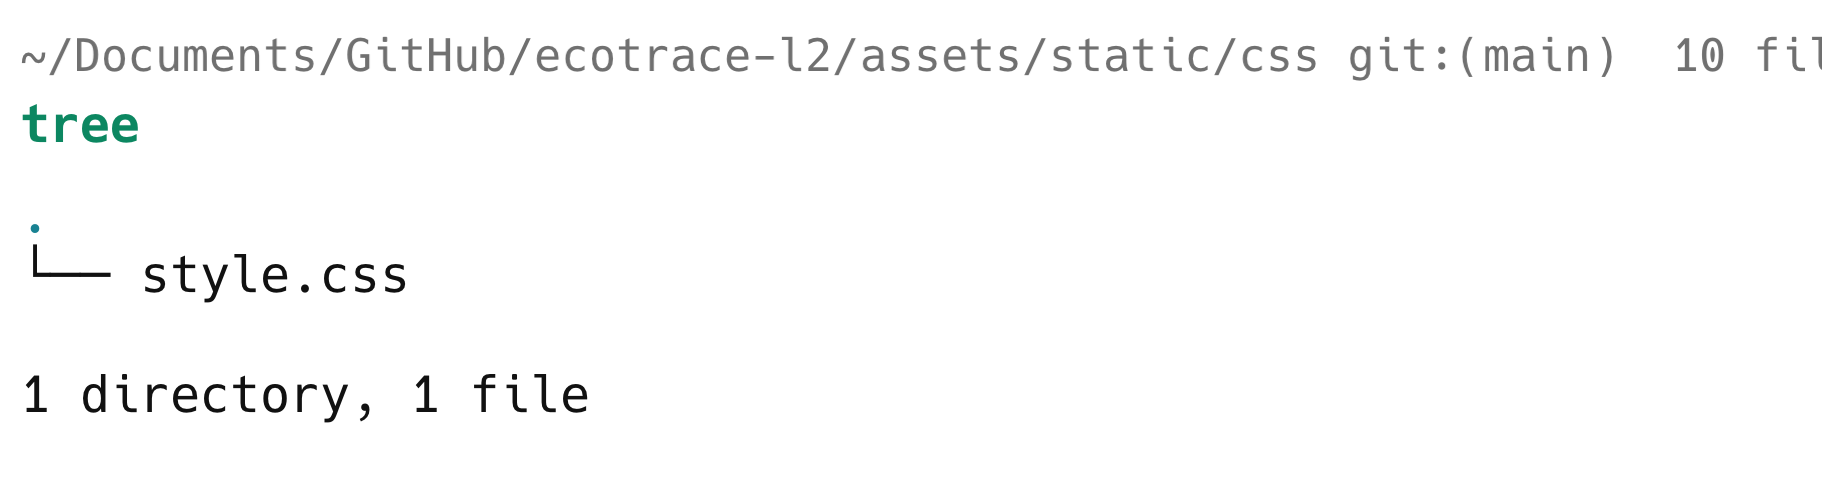
\includegraphics[width=0.7\textwidth]{captures/templates_et_static/static/css/img1.png}
                \end{center}

            \subsection{La fonte personnalisée Inter (\texttt{static/fonts/})}
                \noindent J'ai intégré la fonte Inter, une police moderne et lisible, pour améliorer l'expérience utilisateur. Elle est chargée via le fichier CSS et utilisée dans toute l'application.

            \subsection{Les favicons (\texttt{static/favicon/})}
                \noindent Les favicons sont des petites icônes qui représentent l'application dans les onglets du navigateur. J'ai inclus plusieurs tailles pour assurer une bonne visibilité sur tous les appareils.

    % PARTIE VI: SERVIR L'APPLICATION
        \newpage

        \section{PARTIE VI: Servir l'application}
            \subsection{Architecture de déploiement}
                \noindent Pour mettre en service \textbf{EcoTrace}, j'ai adopté une approche flexible qui facilite aussi bien le développement local que le déploiement en production. L'application repose sur Flask comme serveur web, avec une configuration adaptable selon l'environnement.

            \subsection{Test en local}
                \subsubsection{Fichier de lancement (\texttt{run\_app.py})}
                    \noindent J'ai mis en place un point d'entrée simple et efficace pour l'application :
                    \begin{tcolorbox}[colback=lightgray!6, colframe=black, left=-45mm, right=5mm, top=2mm, bottom=0mm, boxrule=0.1mm]
                        \begin{verbatim}
                            from configs.settings import app

                            if __name__ == "__main__":
                                app.run(debug=False)
                        \end{verbatim}
                    \end{tcolorbox}

                    \noindent Cette méthode présente plusieurs avantages :
                    \begin{itemize}
                        \item Simplicité : Un point d'entrée unique et clair
                        \item Configuration centralisée : Toute la configuration est gérée dans le module \texttt{configs.settings}
                        \item Sécurité : Le mode debug est désactivé par défaut pour une configuration plus sûre
                    \end{itemize}

                \subsubsection{Configuration pour le développement}
                    \noindent Pour le développement local, il est possible d'utiliser :

                    \begin{tcolorbox}[colback=lightgray!6, colframe=black, left=-50mm, right=5mm, top=2mm, bottom=0mm, boxrule=0.1mm]
                        \begin{verbatim}
                            if __name__ == "__main__":
                                app.run(debug=True, host='127.0.0.1', port=5000)
                        \end{verbatim}
                    \end{tcolorbox}

                    \noindent Cependant, j'ai préféré conserver \texttt{debug=False} afin de rester au plus proche des conditions de production.

                    \noindent Voici les étapes pour lancer l'application en local :

                    \begin{enumerate}
                        \item \textbf{Création de l'environnement virtuel et installation des dépendances} :
                            \begin{tcolorbox}[colback=lightgray!6, colframe=black, left=-60mm, right=5mm, top=2mm, bottom=0mm, boxrule=0.1mm]
                                \begin{verbatim}
                                    python -m venv venv
                                    source venv/bin/activate

                                    pip install -r requirements.txt
                                \end{verbatim}
                            \end{tcolorbox}

                        \item \textbf{Lancement de l'application} :
                            \begin{tcolorbox}[colback=lightgray!6, colframe=black, left=-60mm, right=5mm, top=2mm, bottom=0mm, boxrule=0.1mm]
                                \begin{verbatim}
                                    python run_app.py
                                \end{verbatim}
                            \end{tcolorbox}

                        \item \textbf{Accès à l'application} :
                            \begin{tcolorbox}[colback=lightgray!6, colframe=black, left=-60mm, right=5mm, top=2mm, bottom=0mm, boxrule=0.1mm]
                                \begin{verbatim}
                                    http://127.0.0.1:5000
                                \end{verbatim}
                            \end{tcolorbox}

                            \begin{center}
                                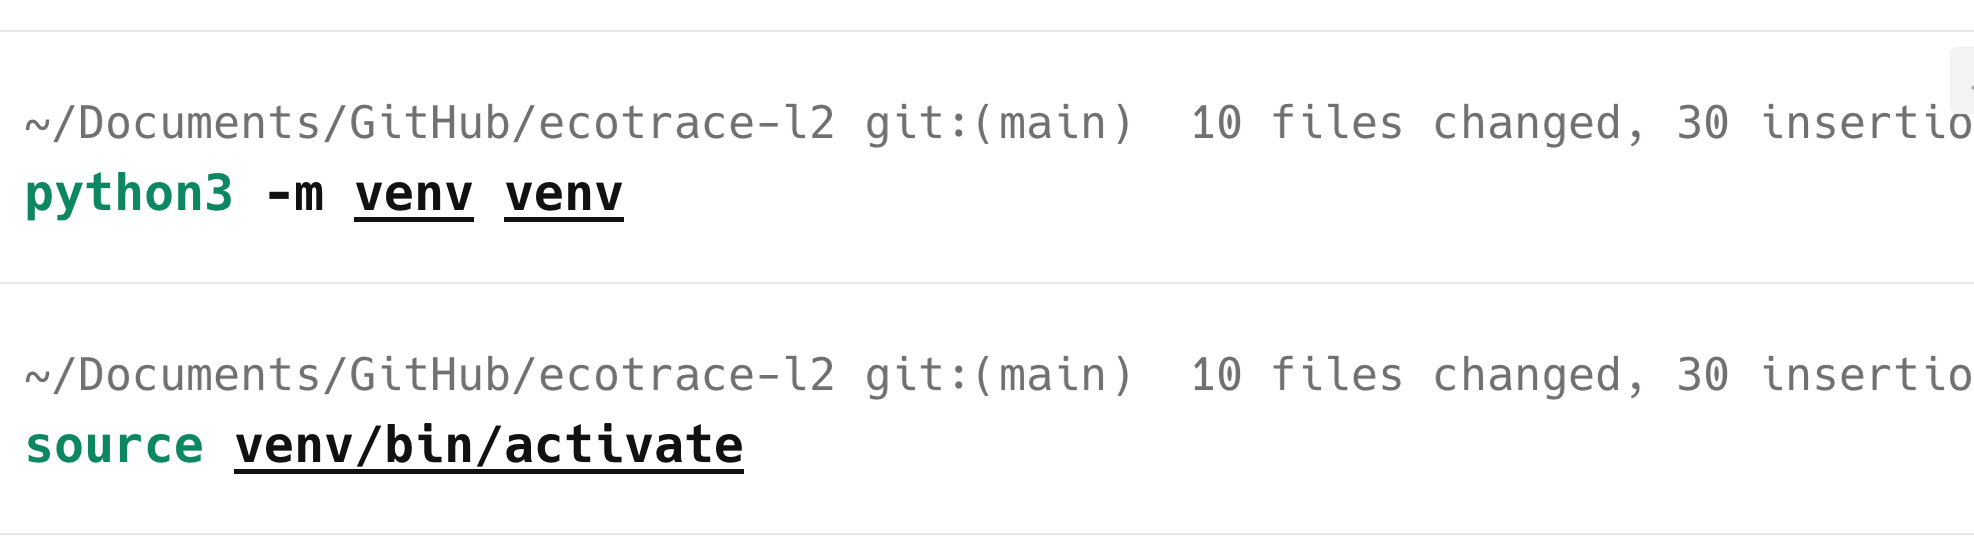
\includegraphics[width=0.7\textwidth]{captures/servir/dev/img1.png}
                            \end{center}
                            \begin{center}
                                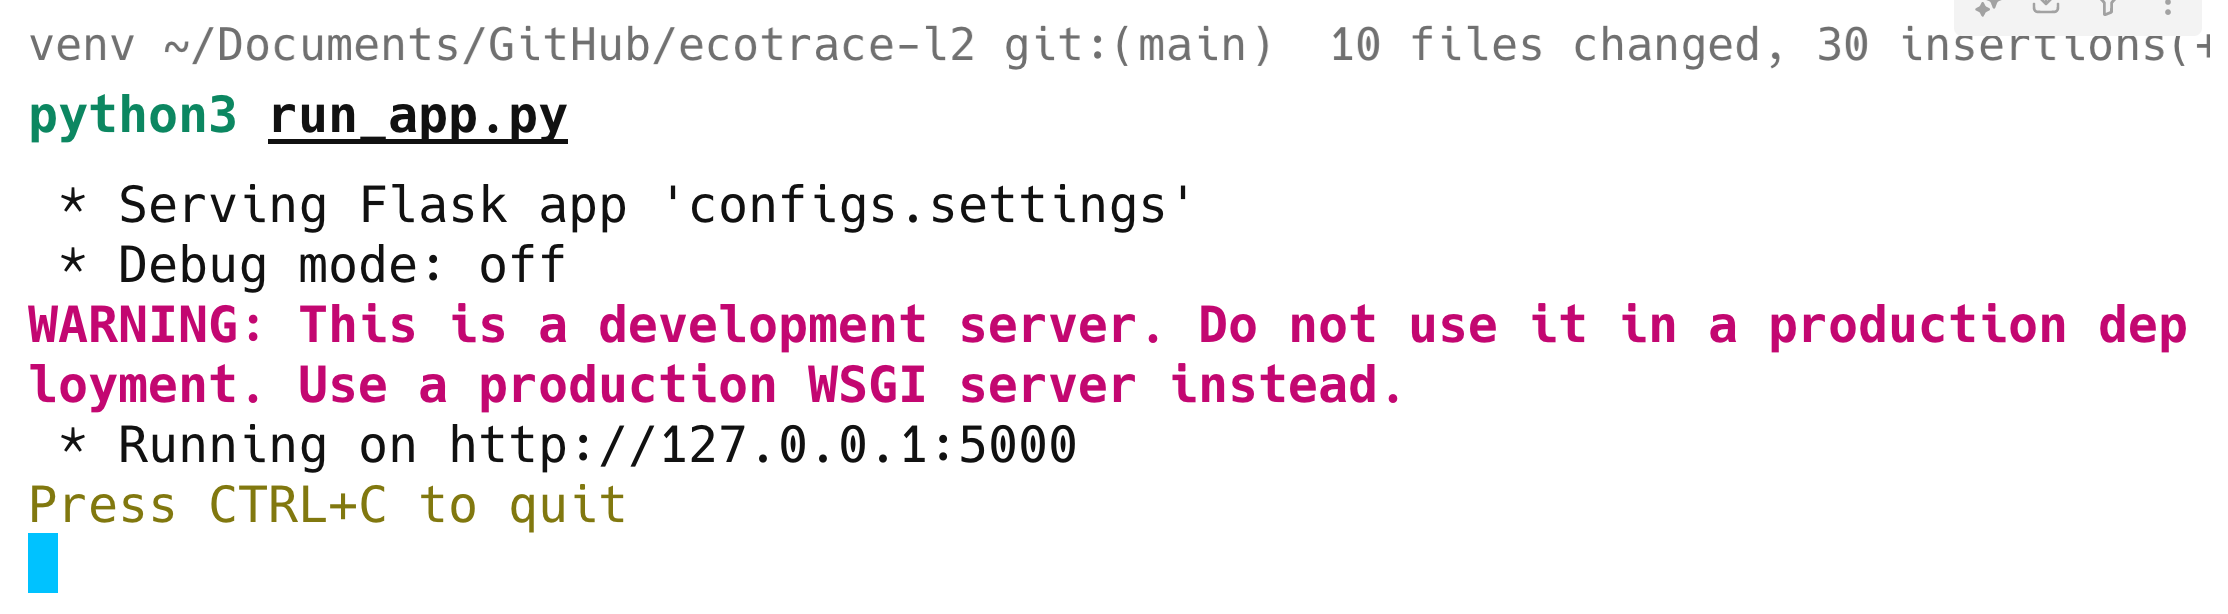
\includegraphics[width=0.7\textwidth]{captures/servir/dev/img2.png}
                            \end{center}

                            \noindent L'application est alors accessible à l'adresse \texttt{http://127.0.0.1:5000}

                            \begin{center}
                                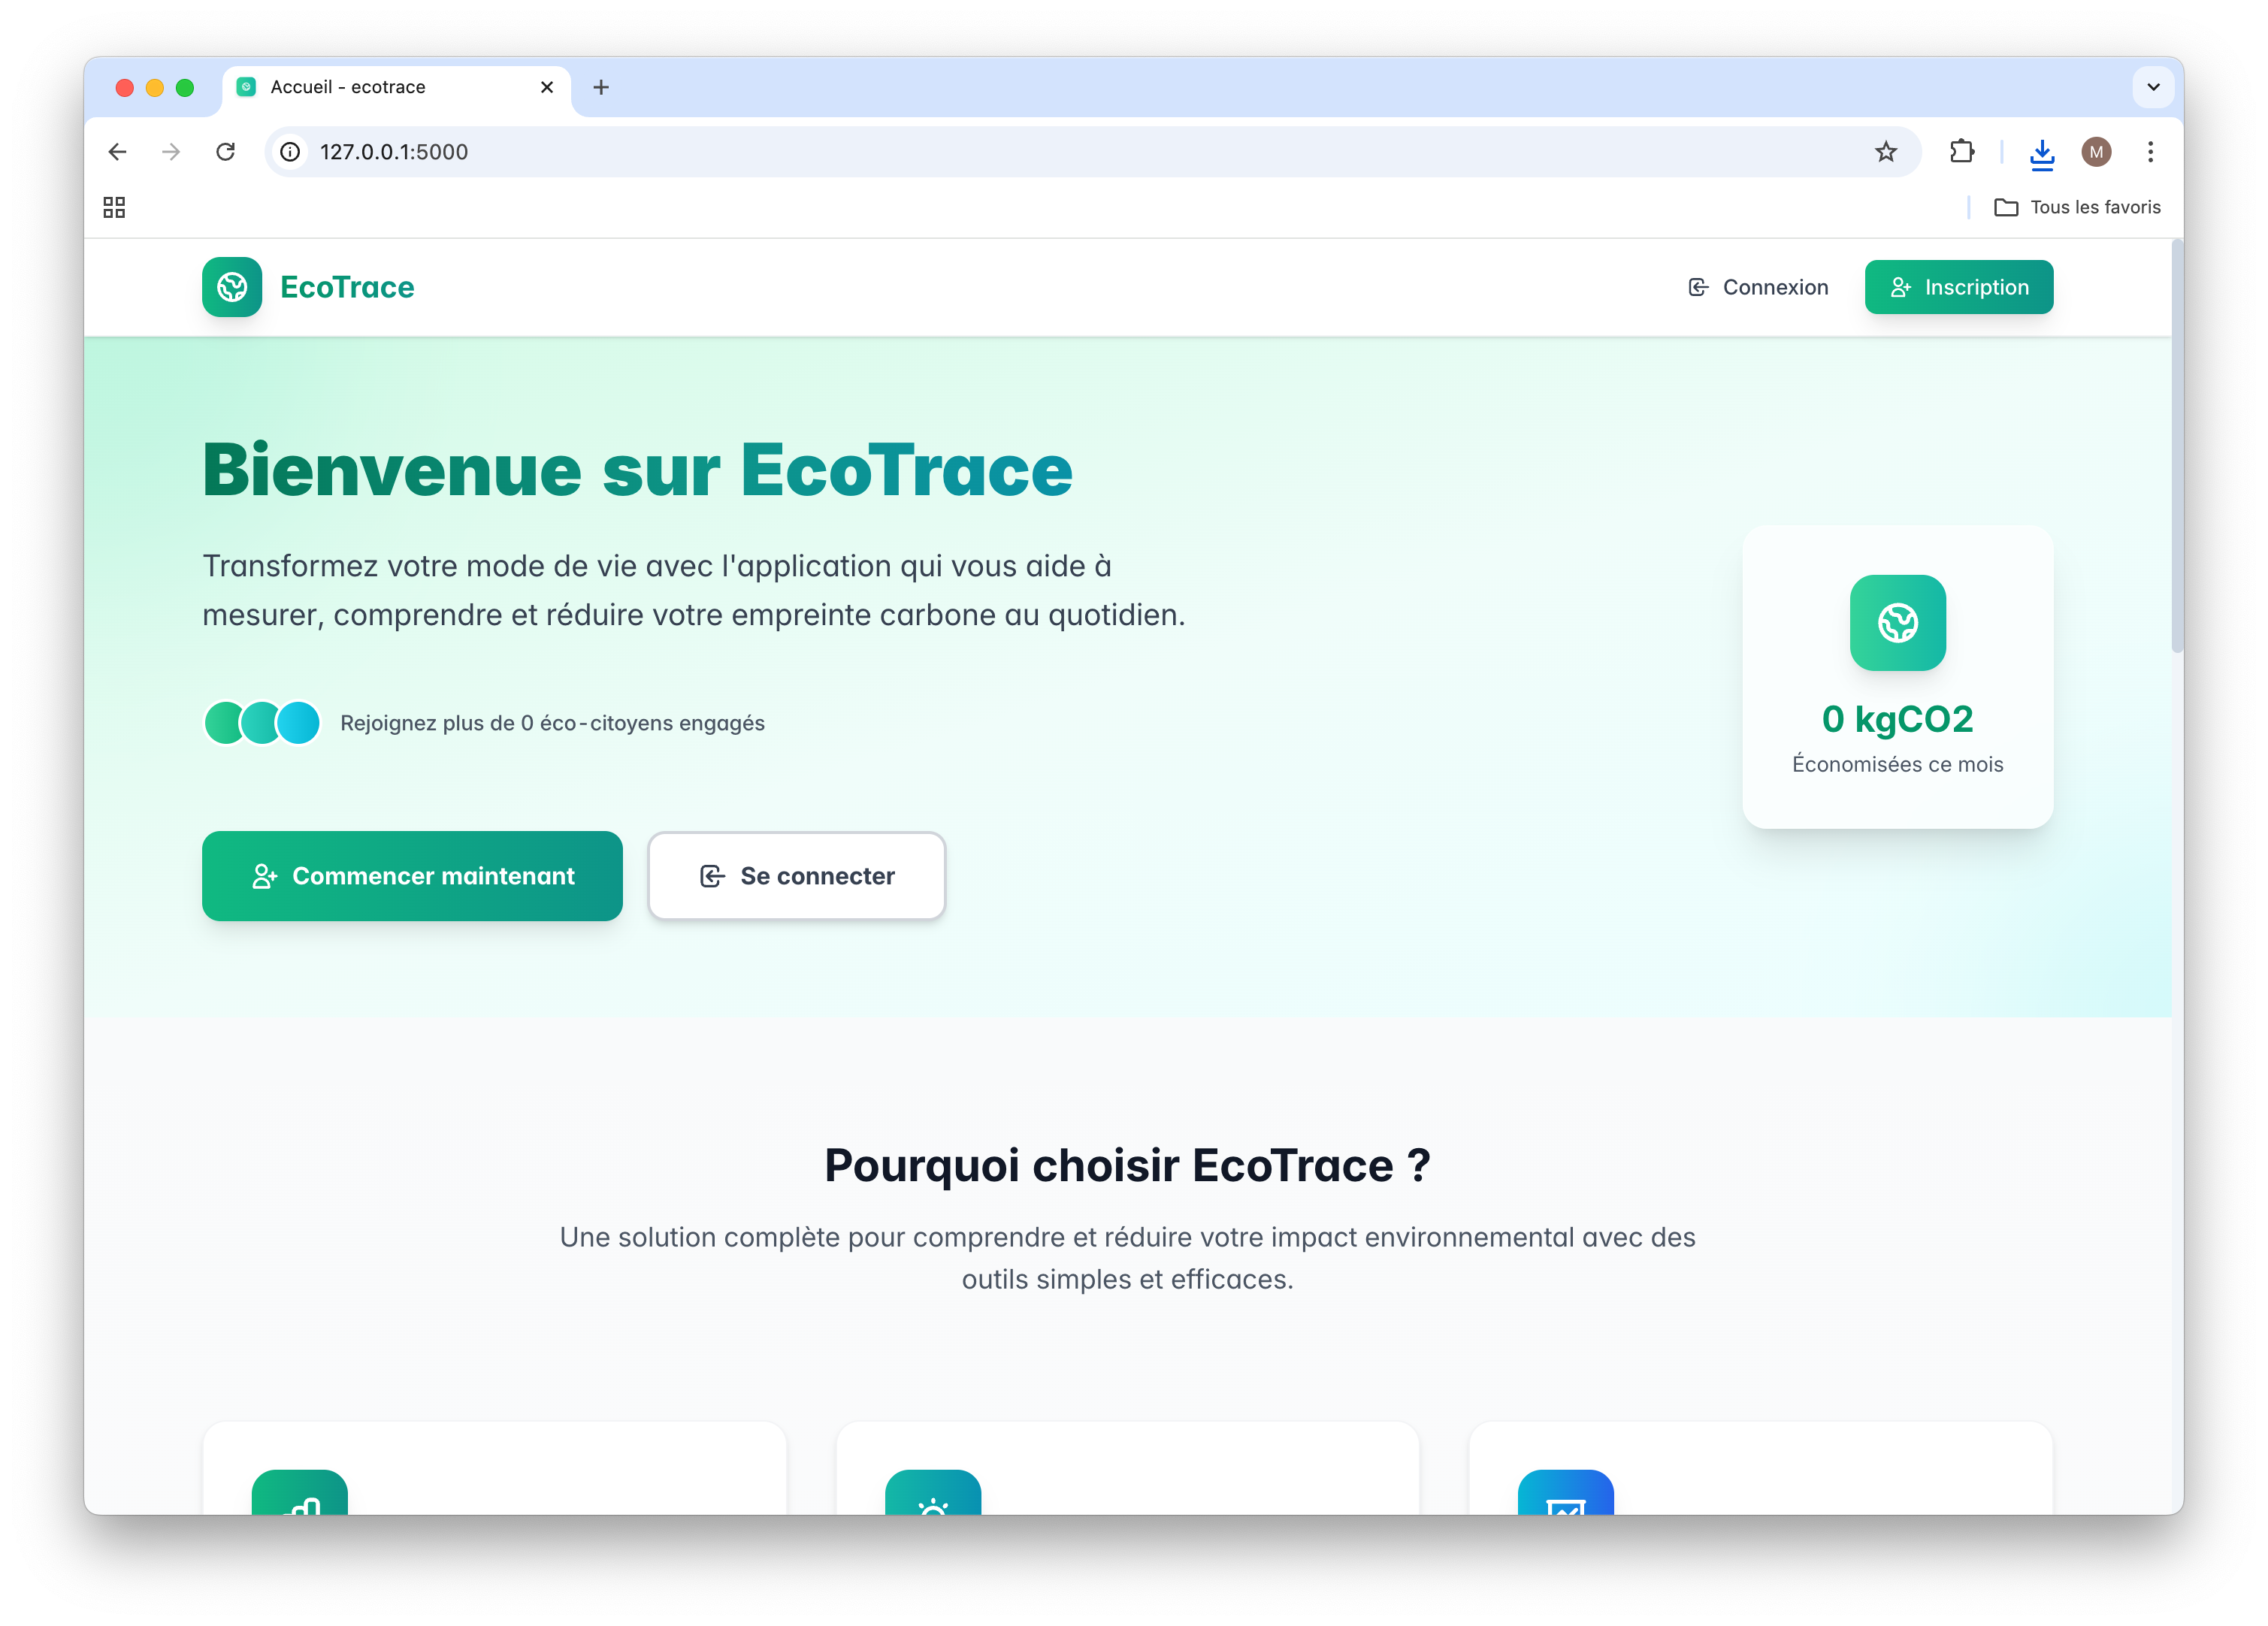
\includegraphics[width=0.7\textwidth]{captures/servir/dev/img4.png}
                            \end{center}
                    \end{enumerate}

            \subsubsection{Mise en production : Déploiement sur PythonAnywhere (offre gratuite)}
                \noindent J'ai choisi PythonAnywhere pour déployer EcoTrace en production. Cette plateforme propose un hébergement Python gratuit, parfaitement adapté aux applications Flask. L'application est accessible à l'adresse : \url{https://ecotrace.pythonanywhere.com}

                \begin{enumerate}
                    \item \textbf{Préparation du code}
                        \begin{tcolorbox}[colback=lightgray!6, colframe=black, left=-50mm, right=5mm, top=2mm, bottom=0mm, boxrule=0.1mm]
                            \begin{verbatim}
                                # Vérification que tous les fichiers sont prêts
                                git add .
                                git commit -m "Préparation pour déploiement PythonAnywhere"
                                git push origin main
                            \end{verbatim}
                        \end{tcolorbox}

                    \item \textbf{Création du compte PythonAnywhere} :
                        \begin{itemize}
                            \item Inscription sur pythonanywhere.com avec l'offre gratuite
                            \item Accès au tableau de bord PythonAnywhere
                            \item Ouverture d'une console Bash
                        \end{itemize}

                    \item \textbf{Upload du code}
                        \begin{tcolorbox}[colback=lightgray!6, colframe=black, left=-50mm, right=5mm, top=2mm, bottom=0mm, boxrule=0.1mm]
                            \begin{verbatim}
                                # Dans la console PythonAnywhere
                                git clone https://github.com/codewithmpia/ecotrace-l2.git
                                cd ecotrace-l2
                            \end{verbatim}
                        \end{tcolorbox}

                    \item \textbf{Création de l'environnement virtuel et installation des dépendances}
                        \begin{tcolorbox}[colback=lightgray!6, colframe=black, left=-50mm, right=5mm, top=2mm, bottom=0mm, boxrule=0.1mm]
                            \begin{verbatim}
                                # Dans la console PythonAnywhere
                                python -m venv venv
                                source venv/bin/activate
                                pip install -r requirements.txt
                            \end{verbatim}
                        \end{tcolorbox}

                    \item \textbf{Configuration WSGI : création du fichier \texttt{/var/www/ecotrace\_pythonanywhere\_com\_wsgi.py}}
                        \begin{tcolorbox}[colback=lightgray!6, colframe=black, left=-50mm, right=5mm, top=2mm, bottom=0mm, boxrule=0.1mm]
                            \begin{verbatim}
                                import sys
                                import os

                                # Ajout du chemin vers votre application
                                path = '/home/ecotrace/ecotrace-l2'
                                if path not in sys.path:
                                    sys.path.append(path)

                                # Import de l'application Flask
                                from configs.settings import app as application
                            \end{verbatim}
                        \end{tcolorbox}

                    \item \textbf{Configuration de l'application web}
                        \begin{itemize}
                            \item Accéder à l'onglet "Web" dans le tableau de bord
                            \item Créer une nouvelle web app Flask
                            \item Définir le chemin source : \texttt{/home/ecotrace/ecotrace-l2}
                            \item Indiquer le fichier WSGI : \texttt{/var/www/ecotrace\_pythonanywhere\_com\_wsgi.py}
                        \end{itemize}

                    \item \textbf{Configuration des fichiers statiques}
                        \begin{tcolorbox}[colback=lightgray!6, colframe=black, left=-50mm, right=5mm, top=2mm, bottom=0mm, boxrule=0.1mm]
                            \begin{verbatim}
                                # Dans l'onglet "Static files"
                                URL: /static/
                                Directory: /home/ecotrace/ecotrace-l2/assets/static/
                            \end{verbatim}
                        \end{tcolorbox}

                    \item \textbf{Initialisation de la base de données}
                        \begin{tcolorbox}[colback=lightgray!6, colframe=black, left=-50mm, right=5mm, top=2mm, bottom=0mm, boxrule=0.1mm]
                            \begin{verbatim}
                                # Dans la console PythonAnywhere
                                cd ecotrace-l2
                                python -c "from configs.settings import app, db; 
                                app.app_context().push(); db.create_all()"
                            \end{verbatim}
                        \end{tcolorbox}

                    \item \textbf{Test et lancement}
                        \begin{itemize}
                            \item Cliquer sur "Reload" dans l'onglet Web
                            \item Vérifier que l'application fonctionne à l'adresse fournie
                            \item Tester les fonctionnalités principales
                        \end{itemize}

                    \item \textbf{Avantages de PythonAnywhere pour EcoTrace}
                        \begin{enumerate}
                            \item \underline{Simplicité de déploiement} :
                                \begin{itemize}
                                    \item Aucune configuration serveur complexe
                                    \item Interface web intuitive
                                    \item Support natif de Python et Flask
                                \end{itemize}
                            \item \underline{Offre gratuite suffisante} :
                                \begin{itemize}
                                    \item 512 MB d'espace disque
                                    \item Bande passante adaptée à un projet étudiant
                                    \item Base de données SQLite incluse
                                    \item Domaine \texttt{pythonanywhere.com} fourni
                                \end{itemize}
                            \item \underline{Maintenance simplifiée} :
                                \begin{itemize}
                                    \item Redémarrage facile via l'interface web
                                    \item Console intégrée pour les commandes
                                    \item Accès direct aux logs
                                \end{itemize}
                        \end{enumerate}
                    
                        \noindent EcoTrace fonctionne parfaitement sur PythonAnywhere et démontre qu'il est possible de déployer une application Flask complète et performante avec l'offre gratuite, tout en assurant une expérience utilisateur fluide et fiable.
                \end{enumerate}


    \newpage
    \section{Conclusion et perspectives}
        \begin{tcolorbox}[colback=lightgray!6, colframe=black, left=2mm, right=5mm, top=2mm, bottom=0mm, boxrule=0.1mm]
            Pour conclure, ce projet EcoTrace m’a permis de mettre en pratique de nombreuses compétences en développement web, de la conception de la base de données à la création d’une interface moderne avec Flask et TailwindCSS.\\

            J’ai découvert l’importance de structurer le code en modules pour faciliter la maintenance et l’évolution de l’application. Ce travail m’a aussi sensibilisé aux enjeux de l’écologie et à la façon dont le numérique peut aider chacun à agir concrètement.\\

            Je suis fier d’avoir pu déployer une application fonctionnelle en ligne et je pense que ce projet pourrait être enrichi avec des fonctionnalités collaboratives ou des données en temps réel.\\

            Cette expérience m’a donné envie de continuer à développer des outils utiles pour la société et d’approfondir mes connaissances en programmation.\\

            Le site est désormais accessible à l'adresse : \url{https://ecotrace.pythonanywhere.com}, et le code source est disponible sur GitHub : \url{https://github.com/codewithmpia/ecotrace-l2}.
        \end{tcolorbox}

    % Difficultés rencontrées
    \newpage
    \section{Difficultés rencontrées}
        \subsection{Difficultés techniques}
            \subsubsection{Gestion des facteurs d'émission}
                \begin{itemize}
                    \item \textbf{Problème} : Intégration et structuration des données ADEME dans la base de données
                    \item \textbf{Défis} : 
                        \begin{itemize}
                            \item Conversion des unités hétérogènes (km, kg, kWh, unités)
                            \item Catégorisation cohérente des activités
                            \item Gestion des valeurs manquantes ou incomplètes
                        \end{itemize}
                    \item \textbf{Solution adoptée} : Création d'un système de facteurs d'émission pré-intégrés avec validation et fallbacks
                \end{itemize}

            \subsubsection{Architecture des dropdowns personnalisés}
                \begin{itemize}
                    \item \textbf{Problème} : Les éléments \texttt{<select>} HTML natifs sont difficiles à styliser avec TailwindCSS
                    \item \textbf{Défis} :
                        \begin{itemize}
                            \item Maintien de l'accessibilité avec des composants personnalisés
                            \item Gestion des événements clavier (Tab, Échap, Entrée)
                            \item Synchronisation entre l'affichage et les valeurs de formulaire
                        \end{itemize}
                    \item \textbf{Solution adoptée} : Développement de dropdowns entièrement personnalisés en JavaScript avec délégation d'événements
                \end{itemize}

            \subsubsection{Calendrier personnalisé}
                \begin{itemize}
                    \item \textbf{Problème} : Les input de type \texttt{date} ne sont pas uniformément supportés et stylisés
                    \item \textbf{Défis} :
                        \begin{itemize}
                            \item Calcul correct des jours du mois et des premières/dernières semaines
                            \item Gestion des années bissextiles
                            \item Positionnement dynamique pour éviter les débordements de viewport
                            \item Localisation en français
                        \end{itemize}
                    \item \textbf{Solution adoptée} : Implémentation d'un calendrier complet en JavaScript avec détection de positionnement automatique
                \end{itemize}

        \subsection{Difficultés d'architecture}

            \subsubsection{Séparation des responsabilités}
                \begin{itemize}
                    \item \textbf{Problème} : Éviter la duplication de code entre les vues et maintenir une logique métier séparée
                    \item \textbf{Défis} :
                        \begin{itemize}
                            \item Centralisation des calculs carbone sans créer de dépendances circulaires
                            \item Réutilisation des méthodes de validation
                            \item Gestion des erreurs cohérente à travers l'application
                        \end{itemize}
                    \item \textbf{Solution adoptée} : Création du module \texttt{controllers} avec classes spécialisées (CarbonCalculator, RecommendationEngine)
                \end{itemize}

            \subsubsection{Gestion des états et des erreurs}
                \begin{itemize}
                    \item \textbf{Problème} : Maintenir la cohérence des données et la robustesse face aux erreurs
                    \item \textbf{Défis} :
                        \begin{itemize}
                            \item Validation des données à plusieurs niveaux (frontend, backend, base de données)
                            \item Gestion des cas limites (données manquantes, utilisateurs sans activités)
                            \item Rollback automatique en cas d'erreur de transaction
                        \end{itemize}
                    \item \textbf{Solution adoptée} : Implémentation de blocs try/catch systématiques avec fallbacks et messages utilisateur appropriés
                \end{itemize}

        \subsection{Difficultés d'interface utilisateur}

            \subsubsection{Responsive design complexe}
                \begin{itemize}
                    \item \textbf{Problème} : Adapter l'interface pour mobile, tablette et desktop avec des composants complexes
                    \item \textbf{Défis} :
                        \begin{itemize}
                            \item Transformation des tableaux en cartes pour mobile
                            \item Réorganisation de la navigation sur petits écrans
                            \item Maintien de l'utilisabilité des formulaires complexes
                        \end{itemize}
                    \item \textbf{Solution adoptée} : Approche mobile-first avec composants adaptatifs et breakpoints TailwindCSS
                \end{itemize}

            \subsubsection{Performance des graphiques}
                \begin{itemize}
                    \item \textbf{Problème} : Affichage fluide des visualisations Chart.js avec des datasets importants
                    \item \textbf{Défis} :
                        \begin{itemize}
                            \item Préparation des données côté serveur vs côté client
                            \item Gestion de la mémoire avec des graphiques multiples
                            \item Animations smooth sans impact sur les performances
                        \end{itemize}
                    \item \textbf{Solution adoptée} : Préparation des données en JSON côté serveur et utilisation de Chart.js avec configuration optimisée
                \end{itemize}

        \subsection{Difficultés de déploiement}

            \subsubsection{Configuration PythonAnywhere}
                \begin{itemize}
                    \item \textbf{Problème} : Adaptation de l'application locale pour l'environnement PythonAnywhere
                    \item \textbf{Défis} :
                        \begin{itemize}
                            \item Configuration du fichier WSGI approprié
                            \item Gestion des chemins relatifs vs absolus
                            \item Installation des dépendances dans l'environnement contraint
                            \item Initialisation de la base de données en production
                        \end{itemize}
                    \item \textbf{Solution adoptée} : Création d'un fichier WSGI dédié et adaptation des chemins statiques
                \end{itemize}

            \subsubsection{Limitations de l'offre gratuite}
                \begin{itemize}
                    \item \textbf{Problème} : Optimisation pour les contraintes de l'hébergement gratuit
                    \item \textbf{Défis} :
                        \begin{itemize}
                            \item Limitation CPU et mémoire
                            \item Redémarrage automatique quotidien
                            \item Pas d'accès HTTPS personnalisé
                        \end{itemize}
                    \item \textbf{Solution adoptée} : Optimisation du code, réduction des requêtes base de données, et acceptation des limitations pour un projet étudiant
                \end{itemize}

        \subsection{Difficultés de données}

            \subsubsection{Cohérence des facteurs d'émission}
                \begin{itemize}
                    \item \textbf{Problème} : Harmonisation des données ADEME avec la structure de l'application
                    \item \textbf{Défis} :
                        \begin{itemize}
                            \item Différences d'unités entre les sources
                            \item Granularité variable des données (générique vs spécifique)
                            \item Mise à jour et versioning des facteurs d'émission
                        \end{itemize}
                    \item \textbf{Solution adoptée} : Création d'une base de données normalisée avec facteurs prévalidés et système de catégories cohérent
                \end{itemize}

        \subsection{Leçons apprises}

            \subsubsection{Planification et architecture}
                \begin{itemize}
                    \item Importance de la définition claire des modèles de données dès le début
                    \item Nécessité d'anticiper les cas d'erreur et les états vides
                    \item Valeur de la séparation stricte entre logique métier et présentation
                \end{itemize}

            \subsubsection{Développement frontend}
                \begin{itemize}
                    \item Avantages des frameworks CSS utility-first comme TailwindCSS
                    \item Complexité des composants interactifs accessibles
                    \item Importance des tests sur différents navigateurs et appareils
                \end{itemize}

            \subsubsection{Déploiement et production}
                \begin{itemize}
                    \item Différences significatives entre environnement de développement et production
                    \item Importance de la documentation des étapes de déploiement
                    \item Nécessité d'anticiper les contraintes d'hébergement
                \end{itemize}

    

    % Sources et Références
    \newpage
    \section{Sources et Références}

    \subsection{Documentation technique}

        \subsubsection{Framework backend}
            \begin{itemize}
                \item Documentation Flask : \url{https://flask.palletsprojects.com/en/2.3.x/}
                \item Documentation SQLAlchemy : \url{https://docs.sqlalchemy.org/en/20/}
                \item Documentation Jinja2 : \url{https://jinja.palletsprojects.com/en/3.1.x/}
            \end{itemize}

        \subsubsection{Extensions Flask}
            \begin{itemize}
                \item Flask-Login : \url{https://flask-login.readthedocs.io/en/latest/}
                \item Flask-WTF : \url{https://flask-wtf.readthedocs.io/en/1.2.x/}
                \item Flask-SQLAlchemy : \url{https://flask-sqlalchemy.palletsprojects.com/en/3.1.x/}
                \item Flask-Minify : \url{https://github.com/mrf345/flask_minify}
            \end{itemize}

    \subsubsection{Frontend et styling}
        \begin{itemize}
            \item Documentation Tailwind CSS : \url{https://tailwindcss.com/docs}
            \item Documentation Chart.js : \url{https://www.chartjs.org/docs/latest/}
            \item Lucide Icons : \url{https://lucide.dev}
        \end{itemize}

    \subsubsection{Hébergement et déploiement}
        \begin{itemize}
            \item PythonAnywhere : \url{https://www.pythonanywhere.com/}
            \item Guide de déploiement Flask : \url{https://help.pythonanywhere.com/pages/Flask/}
        \end{itemize}

    \subsection{Ressources de développement}

        \subsubsection{Outils de développement}
            \begin{itemize}
                \item Git et GitHub pour le versioning
                \item Visual Studio Code comme éditeur
                \item Chrome DevTools pour le débogage frontend
                \item Python virtual environments pour l'isolation des dépendances
            \end{itemize}

        \subsubsection{Bonnes pratiques et patterns}
            \begin{itemize}
                \item Architecture MVC avec Flask
                \item Patterns de sécurité web (CSRF, validation input)
                \item Responsive design principles
                \item Accessibility guidelines (WCAG)
            \end{itemize}

    \subsection{Données et sources scientifiques}

        \subsubsection{Facteurs d'émission carbone}
            \begin{itemize}
                \item Base Carbone® de l'ADEME (\href{https://www.ademe.fr}{Agence de l'Environnement et de la Maîtrise de l'Énergie})
                \item \href{https://www.statistiques.developpement-durable.gouv.fr/lempreinte-carbone-de-la-france-de-1990-2023?rubrique=&dossier=1286}{Données officielles françaises pour les calculs d'empreinte carbone}
                \item \href{https://www.notre-environnement.gouv.fr/themes/climat/les-emissions-de-gaz-a-effet-de-serre-et-l-empreinte-carbone-ressources/article/les-emissions-de-gaz-a-effet-de-serre-du-secteur-des-transports}{Facteurs d'émission par secteur (transport, alimentation, énergie, consommation)}
            \end{itemize}

    \subsection{Inspiration et références design}

        \subsubsection{Design system et UI/UX}
            \begin{itemize}
                \item Material Design principles
                \item Apple Human Interface Guidelines
                \item Figma community resources
                \item Modern web design trends
            \end{itemize}

        \subsubsection{Accessibilité}
            \begin{itemize}
                \item WCAG 2.1 Guidelines
                \item WebAIM resources
                \item Inclusive design principles
            \end{itemize}

    \subsection{Outils et technologies}

        \subsubsection{Bibliothèques JavaScript}
            \begin{itemize}
                \item Chart.js pour la visualisation de données
                \item Vanilla JavaScript pour les interactions
                \item Modern ES6+ features
            \end{itemize}

        \subsubsection{CSS et styling}
            \begin{itemize}
                \item Tailwind CSS utility-first framework
                \item CSS Grid et Flexbox pour les layouts
                \item CSS custom properties pour la théma
            \end{itemize}

        \subsubsection{Développement et qualité}
            \begin{itemize}
                \item Python PEP 8 style guide
                \item HTML5 semantic markup
                \item Progressive enhancement principles
            \end{itemize}
\end{document}
